\chapter{Analysis and results}
%\vspace{\baselineskip}
%\addcontentsline{toc}{section}{Analysis and results}
This chapter presents the results obtained from several simulations and compares them to analyse the differences across scenarios. The model allows to modify and customize several options, such as the population growth rate, the user-speed demand growth rate, the coverage obligations, the way this coverage obligations are enforced, and the capacity expansion strategies that the telecom operator can use to achieve the coverage obligation and meet the demand.\par

There are also some parameters of the code that are fixed a priori such as the overbooking factor of the macrocells, the percentage of traffic in the busy hour, if the operator invests only to meet the coverage obligation or to meet the demand, and if the operator has a limited budget or not. However, these can be modified to analyse the impact of variations of those parameters, too.\par

Regarding the PCDs and LADs, it is important to understand how they are distributed across the country. The following figures represent the population distribution, measured in aggregate population, and the population density distribution, measured in population per km\textsuperscript{2}. The values for each LAD are obtained at the beginning of the simulation (2020) and are equal for all the years. Despite these values vary over time depending on the population and end-user speed growth scenarios, this variation is homogeneous across the territory.\par



%%%%%%%%%%%%%%%%%%%% Figure/Image No: 1 starts here %%%%%%%%%%%%%%%%%%%%

\begin{figure}[H]
	\begin{Center}
		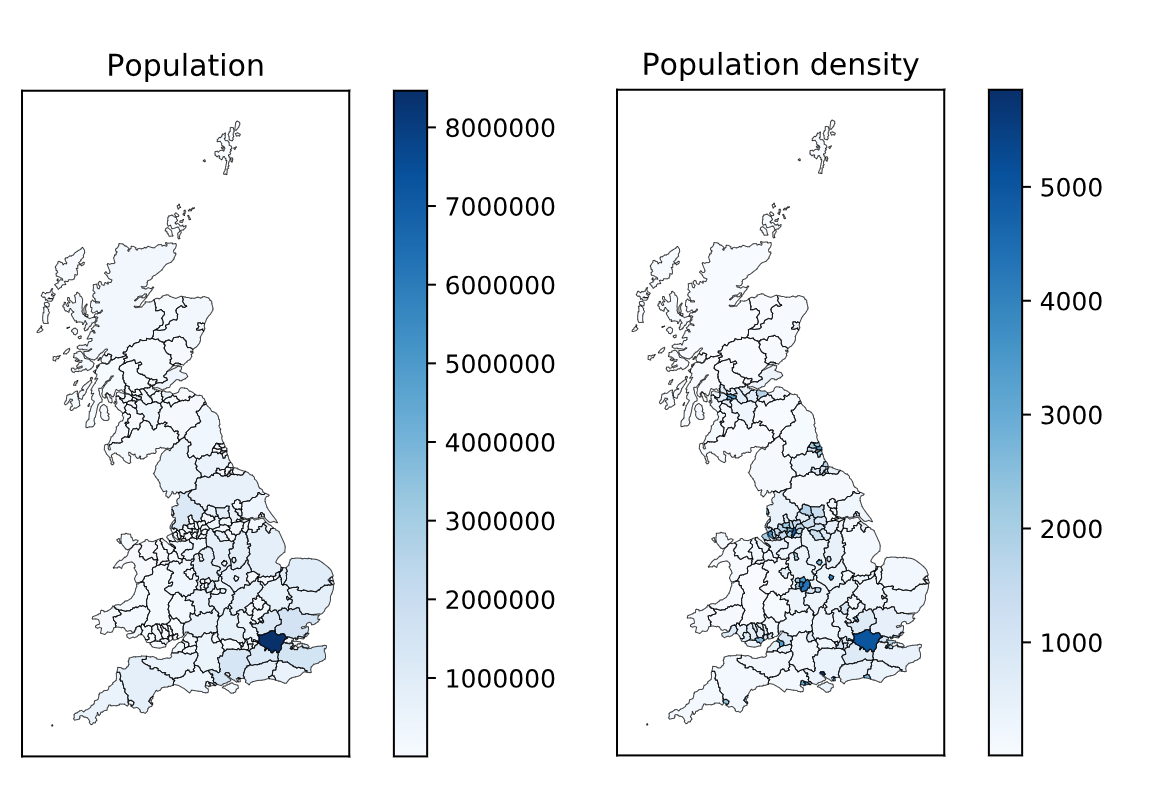
\includegraphics[width=0.95\textwidth]{./media/image40.png}
		\caption{Map. Population and population density. Source: Author}
	\end{Center}
\end{figure}


%%%%%%%%%%%%%%%%%%%% Figure/Image No: 1 Ends here %%%%%%%%%%%%%%%%%%%%

As it can be seen, the population is clearly higher in the London LAD, while the rest of the country have more similar population values (figure on the left). On the contrary, when we consider population density at the LAD, other regions in the UK become more important, matching with most of the important cities of the country: Manchester, Liverpool, Birmingham, Sheffield, Glasgow, etc. \par

In the following sections, I  present the simulations of different scenarios with different capacity expansion strategies and coverage obligation options. First, we evaluate the new capacity expansion strategy, 700 MHz densification. Then, we compare all the capacity expansion strategies and extract the key advantages and disadvantages of each of them. Finally, we test the coverage obligation options using two different strategies in the simulation to analyse how different coverage obligations affect the telecom operator in different ways depending on the strategy.\par


\section{700 MHz densification}
%\subsection*{700 MHz densification}
%\addcontentsline{toc}{subsection}{700 MHz densification}
700 MHz densification is the new intervention created in this Master Thesis. It consists in integrating the 700 MHz band in the existing base stations in the area and, once all of them have 700 MHz carriers, the intervention builds new base stations until the capacity demanded is reached, the coverage obligations are fulfilled, or the maximum site density is reached.\par

After that, I have created a new capacity expansion strategy, the �\textit{700 MHz densification�} that is only allowed to use the �\textit{700 MHz densification�} strategy.\textit{ }The following figures show the effects that using this capacity strategy has on the development of the mobile telecommunications network. \par

\subsection*{Investment}
%\addcontentsline{toc}{subsection}{Investment}
The cost distribution is the first of the two most important outputs to analyse of a simulation. The investment graph shows the evolution of the investment over the years and produces several important results: (i) It allows to check how much it has been spent per year, (ii) how many years the telecom operator exhausted all its budget, (iii) when the capacity cannot be further increased because it has reached the limit of the technology. \par

The following graph represents the investment made by the telecom operator per year to build new assets in all the country. The green line shows in which year the telecom operator starts to invest to satisfy the demand instead of investing to fulfil the coverage obligations. This test uses the baseline population growth scenario, the baseline user-speed growth scenario, and the \textit{�More profitable first�} coverage obligation option with a speed of 2 Mbps. \par



%%%%%%%%%%%%%%%%%%%% Figure/Image No: 2 starts here %%%%%%%%%%%%%%%%%%%%

\begin{figure}[H]
	\begin{Center}
		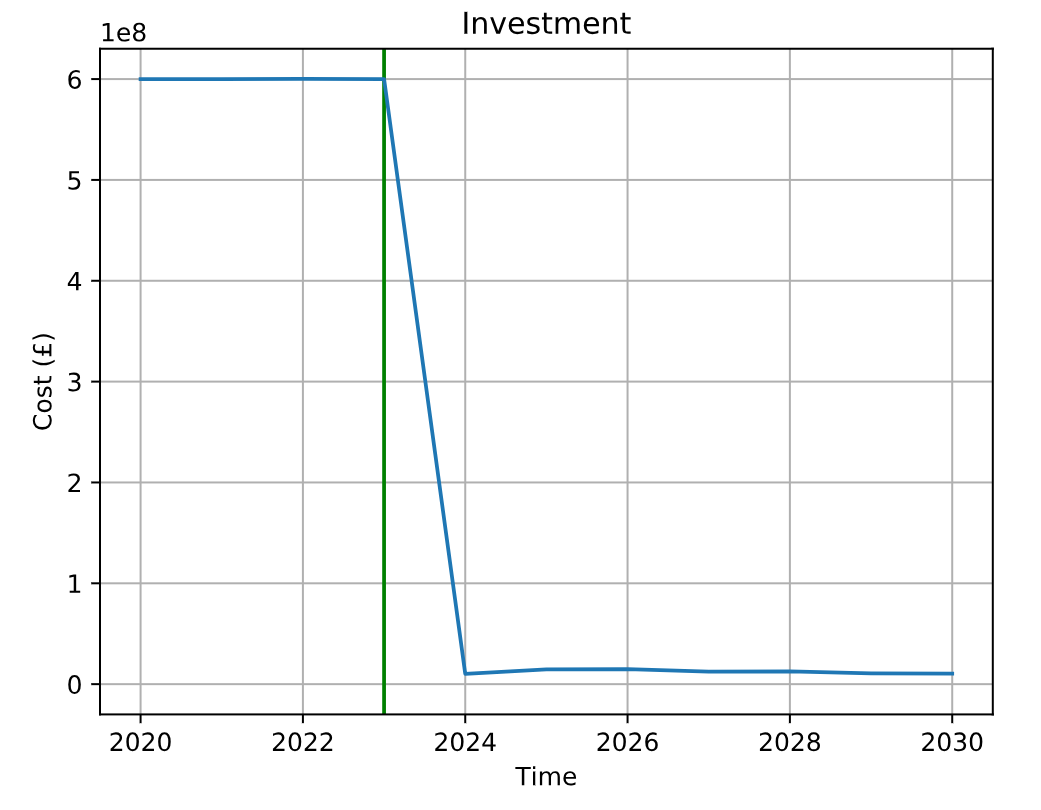
\includegraphics[width=0.85\textwidth]{./media/image41.png}
		\caption{700 MHz densification. Graph: Investment. Source: Author}
	\end{Center}
\end{figure}


%%%%%%%%%%%%%%%%%%%% Figure/Image No: 2 Ends here %%%%%%%%%%%%%%%%%%%%

As it can be seen, the investment is not the same every year. For the first 4 years (from 2020 to 2023) the telecom operator invests all the budget that it has: around �600,000,000. In the year 2023 the investment rate decreases to less than 10$\%$  of the maximum, two things could happen: (i) the telecom operator determines that is fulfilling the coverage obligations and stops investing, (ii) despite some regions still need more investment, it is not possible due to technical limitations. We need the population covered analysis to determine which is the case.\par

Another output that is important is the cost of increasing the population covered using this strategy. It is not linear since each geotype have different propagation characteristics. The following graph shows information related to this output:\par



%%%%%%%%%%%%%%%%%%%% Figure/Image No: 3 starts here %%%%%%%%%%%%%%%%%%%%

\begin{figure}[H]
	\begin{Center}
		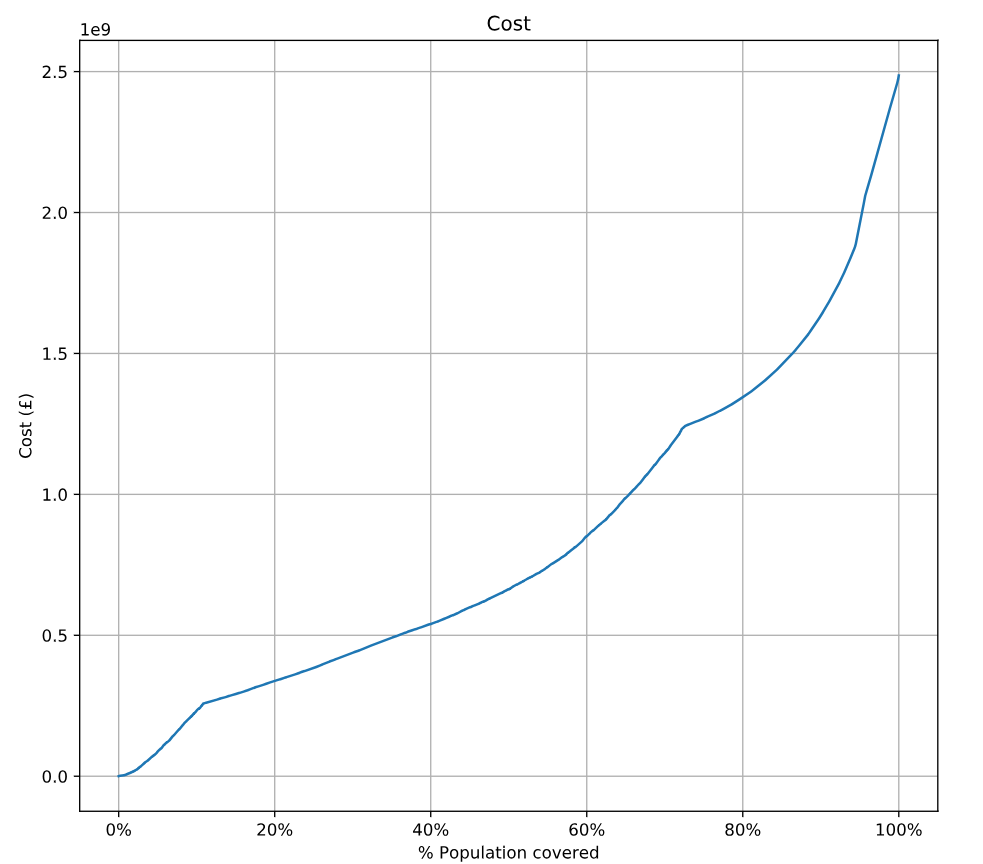
\includegraphics[width=0.95\textwidth]{./media/image42.png}
		\caption{700 MHz densification. Graph: Cost. Source: Author}
	\end{Center}
\end{figure}


%%%%%%%%%%%%%%%%%%%% Figure/Image No: 3 Ends here %%%%%%%%%%%%%%%%%%%%

This test uses the baseline population growth scenario, the baseline user-speed growth scenario, and the \textit{�More profitable first�} coverage obligation option with a speed of 2 Mbps. The graph represents the cumulative costs of having a certain percentage of population covered. It shows an increasing growth of the marginal costs as the coverage increases. The reason is that \textit{�More profitable first�} orders all the PCDs from most to least densely populated, which means that urban PCDs are first and rural PCDs are the last.\par

There are three main parts in which rates of cost increase could be divided: (i) Urban areas (circa 0$\%$  to 10$\%$ ), (ii) suburban areas (circa 10$\%$  to 75$\%$ ), and (iii) rural areas (circa 75$\%$  to 100$\%$ ). Despite the slope of the curve is not constant inside each part, in general terms, the slope is steeper for the rural areas because the population density is so low that the operator has to add ever more antennas. This is not because of capacity needs, but because of the limitation in range of coverage due to the attenuation losses. On the contrary, in highly populated areas, the operator is forced to build a lot of assets, because it needs a lot of capacity, but this strategy raises the costs significantly.\par

Finally, the following coloured map represents the distribution of costs across the country and how the most populated areas, especially London area, receive more investments during all the years:\par



%%%%%%%%%%%%%%%%%%%% Figure/Image No: 4 starts here %%%%%%%%%%%%%%%%%%%%

\begin{figure}[H]
	\begin{Center}
		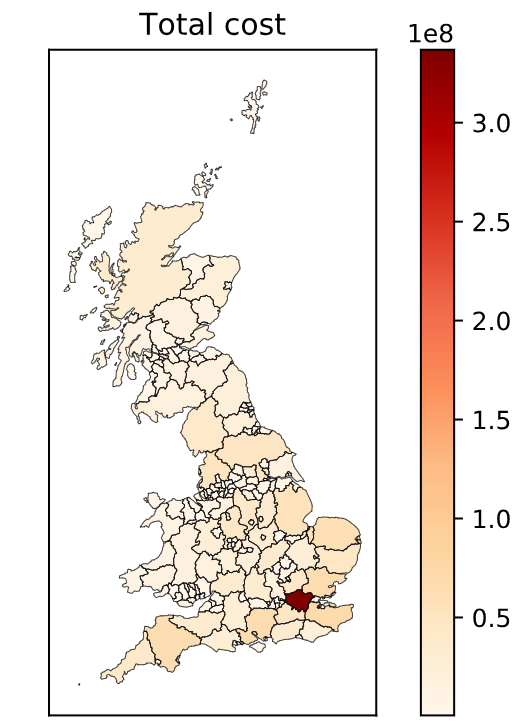
\includegraphics[width=0.65\textwidth]{./media/image43.png}
		\caption{700 MHz densification. Map: Total cost. Source: Author}
	\end{Center}
\end{figure}


%%%%%%%%%%%%%%%%%%%% Figure/Image No: 4 Ends here %%%%%%%%%%%%%%%%%%%%

\subsection*{Population covered}
%\addcontentsline{toc}{subsection}{Population covered}
The population covered over time is the second most important outputs to analyse. The detail per year produces three important results: (I) How the population is covered year by year, (II) If the given run is good enough to satisfy the demand and the coverage obligations in ten years, (III) If there are regions that simply cannot have enough capacity due to several reasons. The following map shows the evolution over time of the percentage of users that have at least the 2Mbps that the coverage obligation forces:\par



%%%%%%%%%%%%%%%%%%%% Figure/Image No: 5 starts here %%%%%%%%%%%%%%%%%%%%

\begin{figure}[H]
	\begin{Center}
		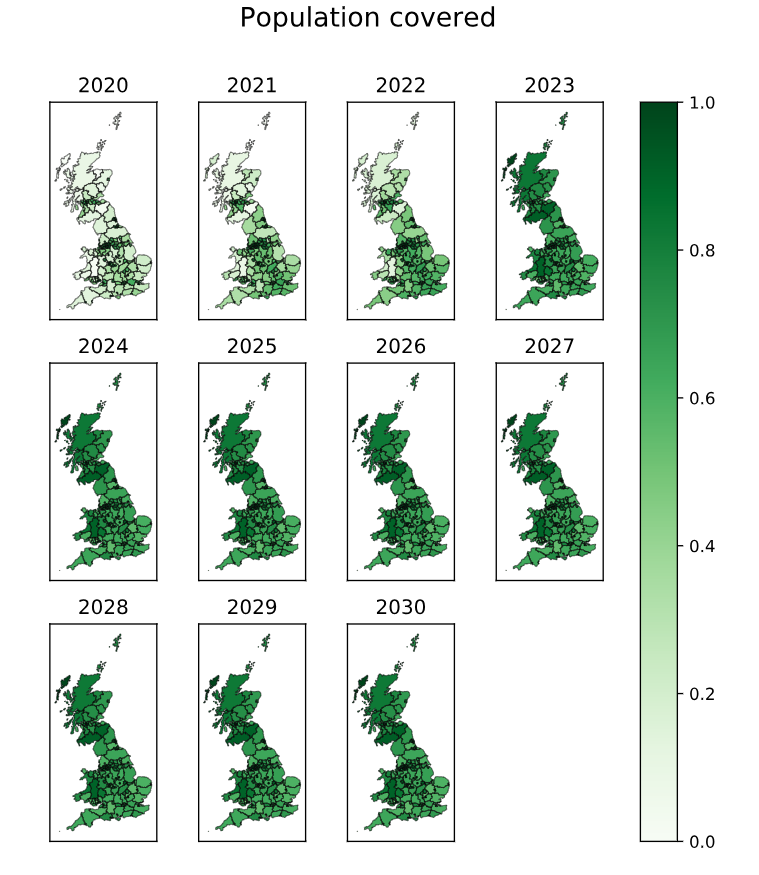
\includegraphics[width=0.95\textwidth]{./media/image44.png}
		\caption{700 MHz densification. Map: Population covered. Source: Author}
	\end{Center}
\end{figure}


%%%%%%%%%%%%%%%%%%%% Figure/Image No: 5 Ends here %%%%%%%%%%%%%%%%%%%%

This map only shows information at a LAD level, but this information will be covered in higher detail in the following graphs. This test uses the baseline population growth scenario, the baseline user-speed growth scenario, and the \textit{�More profitable first�} coverage obligation with a speed of 2 Mbps.\par

As it can be seen, most of the regions do not have enough capacity installed in the beginning and the most populated regions (those that have a bigger percentage) had a larger percentage of population covered. This is where telecom operators normally invest because it is generally more profitable (As the population density is higher, people concentrate in bigger cities and telecom operators can reach more people just with one base station).\par

With this capacity expansion strategy, coverage growths quickly at first, while from 2023 to 2030 it remains approximately similar. The final percentage is considerably better than at the beginning, but it is not 100$\%$  in all the regions. The following histogram shows the distribution of the coverage obligation percentage at the end with a higher detail since it represents the probability of a PCD of having a specific population covered percentage:\par



%%%%%%%%%%%%%%%%%%%% Figure/Image No: 6 starts here %%%%%%%%%%%%%%%%%%%%

\begin{figure}[H]
	\begin{Center}
		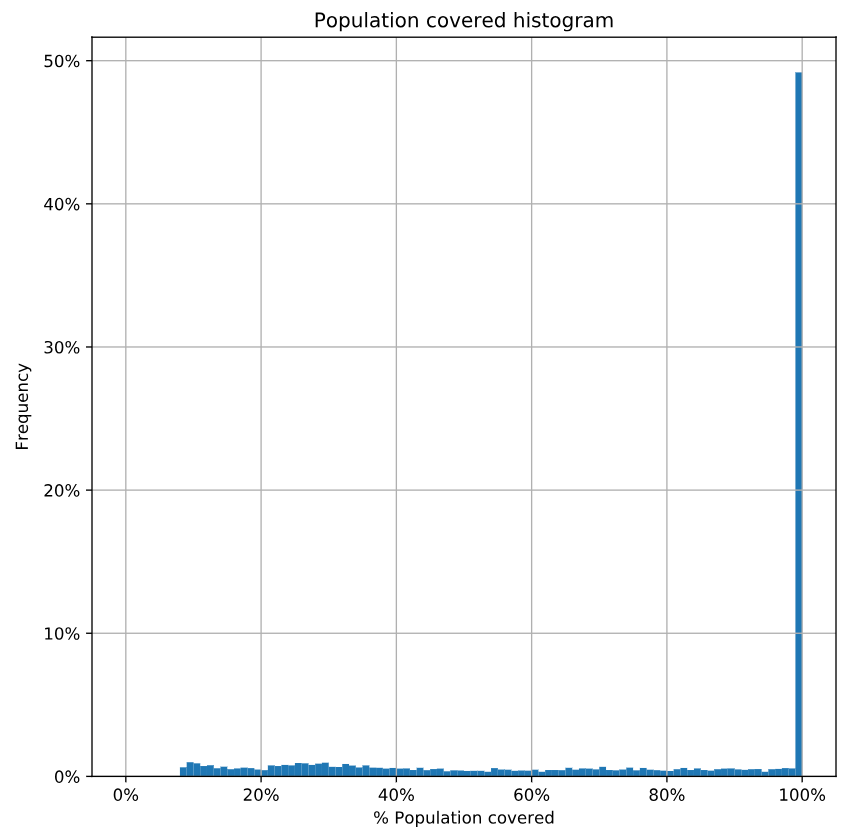
\includegraphics[width=0.80\textwidth]{./media/image45.png}
		\caption{700 MHz densification. Histogram: Population covered. Source: Author}
	\end{Center}
\end{figure}


%%%%%%%%%%%%%%%%%%%% Figure/Image No: 6 Ends here %%%%%%%%%%%%%%%%%%%%

This test uses the baseline population growth scenario, the baseline user-speed growth scenario, and the \textit{�More profitable first�} coverage obligation option with a speed of 2 Mbps. As it can be seen in the histogram, almost half of the PCDs fulfil their coverage obligations completely, but the other half cannot.\par

Combining the results of the histogram with the investment per year graph, it can be inferred that the telecom operator has enough budget to continue with the investments, but it cannot due to technical limitations. In this case, the telecom operator can only use the 700 MHz band and its capacity is limited. Half of the PCDs demand less than the maximum capacity of the band and the rest have only a portion of the coverage obligation fulfilled.\par

\subsection*{Technology upgrades}
%\addcontentsline{toc}{subsection}{Technology upgrades}
The code also allows one to see the technology upgrades of every region of the country. The following chart represents the technology upgrades made using the 700 MHz intervention. It uses the baseline population growth scenario, the baseline user-speed growth scenario, and the \textit{�More profitable first�} coverage obligation with a speed of 2 Mbps. As can be seen, the distribution of the deployment of base stations is not homogeneous since the London region is much more populated than areas from Wales or Scotland.\par



%%%%%%%%%%%%%%%%%%%% Figure/Image No: 7 starts here %%%%%%%%%%%%%%%%%%%%

\begin{figure}[H]
	\begin{Center}
		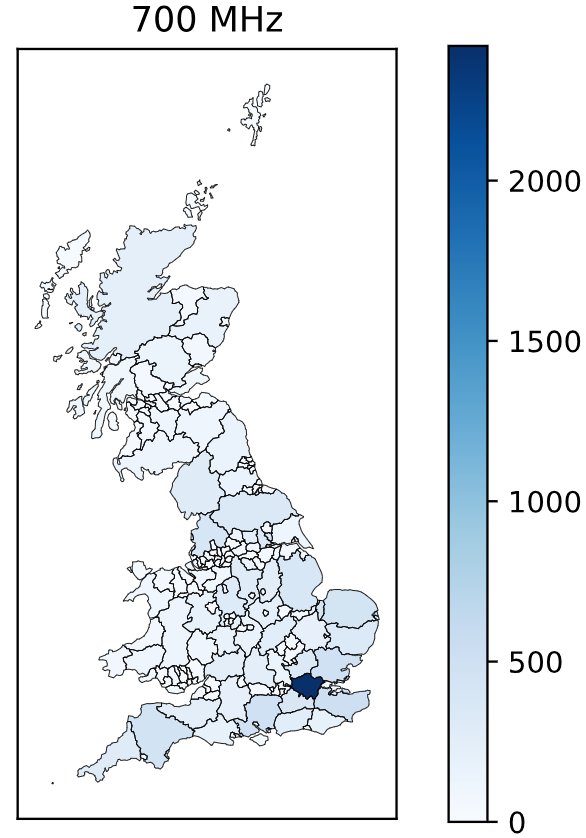
\includegraphics[width=0.50\textwidth]{./media/image46.png}
		\caption{700 MHz densification. Map: Technology upgrades. Source: Author}
	\end{Center}
\end{figure}


%%%%%%%%%%%%%%%%%%%% Figure/Image No: 7 Ends here %%%%%%%%%%%%%%%%%%%%

\subsection*{Capacity margin}
%\addcontentsline{toc}{subsection}{Capacity margin}
The section �Population Covered� discussed the\ relation between the capacity installed and the coverage obligation. Now, we study the capacity and demand parameters and its relation, the capacity margin.  The following coloured map represents the evolution of the capacity along the years.\par



%%%%%%%%%%%%%%%%%%%% Figure/Image No: 8 starts here %%%%%%%%%%%%%%%%%%%%

\begin{figure}[H]
	\begin{Center}
		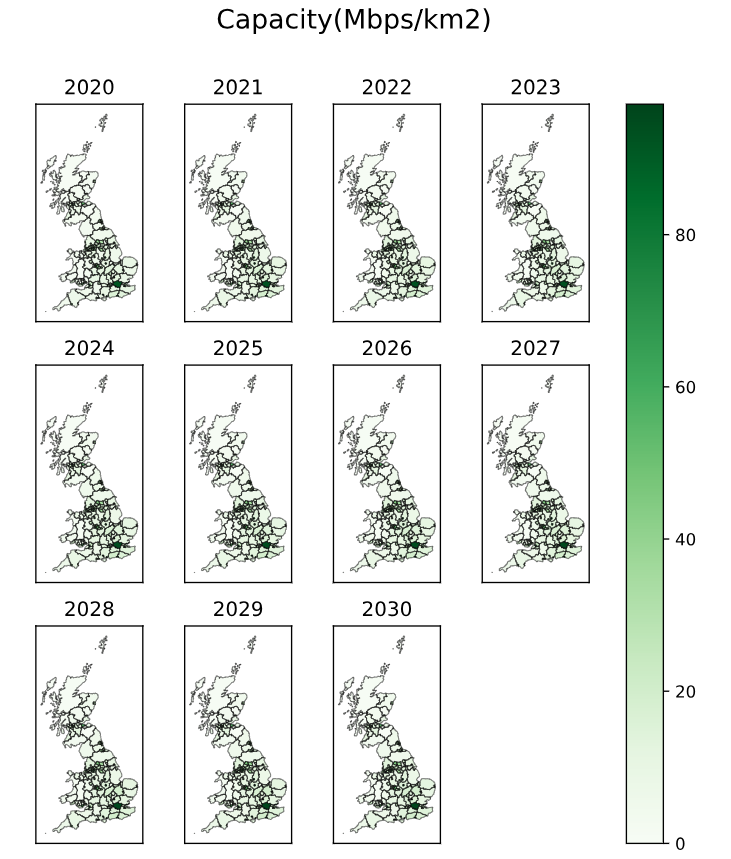
\includegraphics[width=0.9\textwidth]{./media/image47.png}
		\caption{700 MHz densification. Map: Capacity evolution. Source: Author}
	\end{Center}
\end{figure}


%%%%%%%%%%%%%%%%%%%% Figure/Image No: 8 Ends here %%%%%%%%%%%%%%%%%%%%

This map is calculated using the baseline population growth scenario, the baseline user-speed growth scenario, and the \textit{�More profitable first�} coverage obligation with a speed of 2 Mbps. It represents the capacity in Mbps per km\textsuperscript{2} installed at the end of each year and allows to see the evolution of the investment but also to see how much capacity was installed in each region at the beginning of the simulation. Note that if the reader wants to back-calculate the maximum population that could be satisfied using a capacity of 50 Mbps per km\textsuperscript{2} the conversion is not direct since they should consider the overbooking factor, the market share of the operator, etc. The following map represents the evolution of the demand over the years using the same simulation:\par



%%%%%%%%%%%%%%%%%%%% Figure/Image No: 9 starts here %%%%%%%%%%%%%%%%%%%%

\begin{figure}[H]
	\begin{Center}
		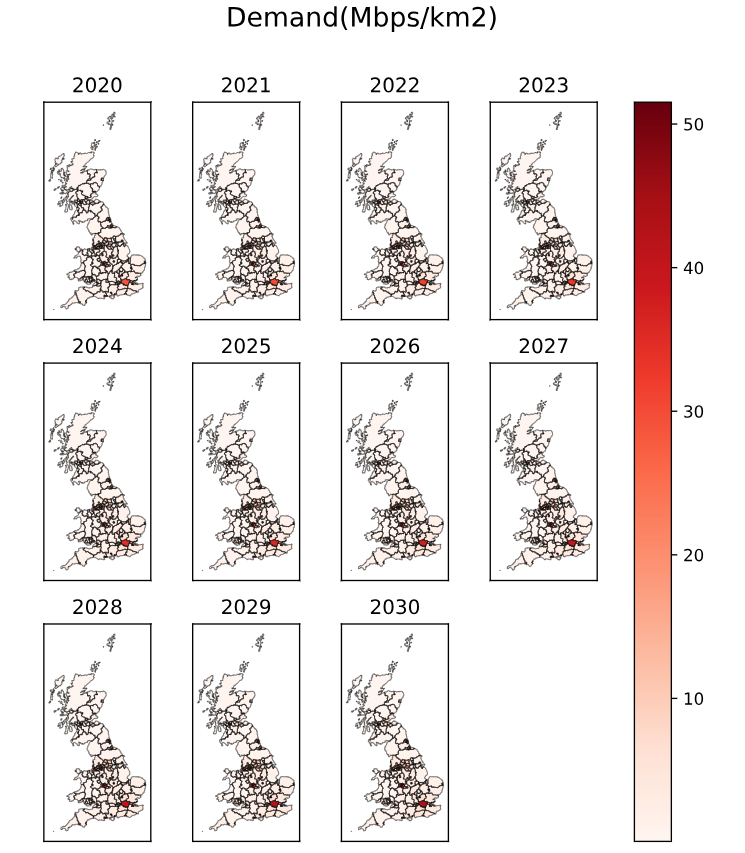
\includegraphics[width=0.90\textwidth]{./media/image48.png}
		\caption{700 MHz densification. Map: Demand evolution. Source: Author}
	\end{Center}
\end{figure}


%%%%%%%%%%%%%%%%%%%% Figure/Image No: 9 Ends here %%%%%%%%%%%%%%%%%%%%

Finally, the following coloured map calculates the subtraction of the demand from the capacity values and represents the amount of capacity in Mbps per km\textsuperscript{2} that each region lacks or has extra. This is the value that, without coverage obligations, the telecom operators normally use to check which are the highest priority areas to invest.\par


%%%%%%%%%%%%%%%%%%%% Figure/Image No: 10 starts here %%%%%%%%%%%%%%%%%%%%

\begin{figure}[H]
	\begin{Center}
		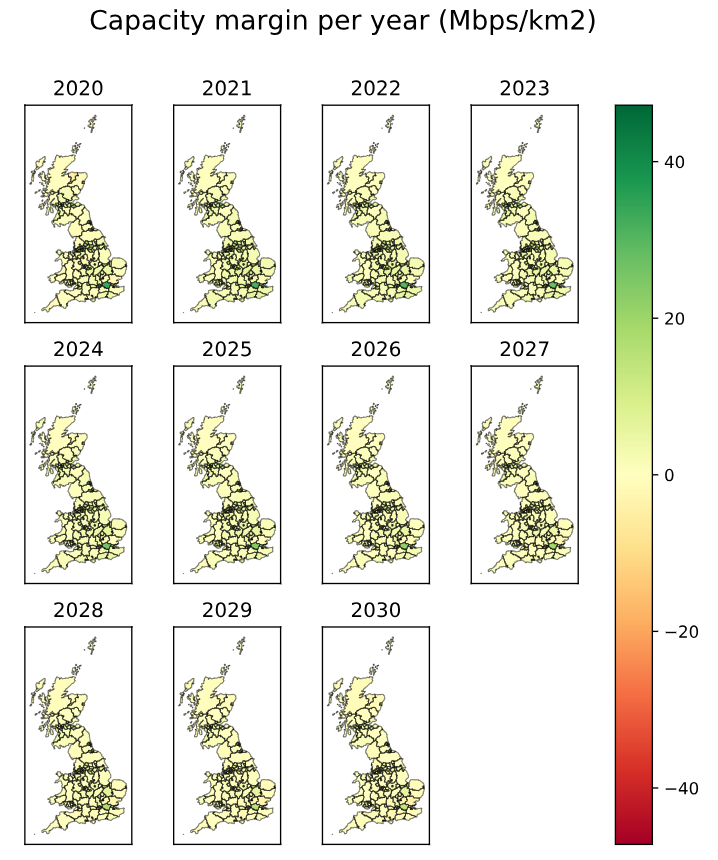
\includegraphics[width=0.90\textwidth]{./media/image49.png}
		\caption{700 MHz densification. Map: Capacity margin evolution. Source: Author}
	\end{Center}
\end{figure}


%%%%%%%%%%%%%%%%%%%% Figure/Image No: 10 Ends here %%%%%%%%%%%%%%%%%%%%
\subsection*{Total costs}
%\addcontentsline{toc}{subsection}{Total costs}
The previous analysis was executed considering that the telecom operator has a limited amount of money available to invest every year. As we want to be sure if the operator is limited by investment force or technical requirements, I have run a new execution of the code without limits in the annual budget and the results are the same. The problem of using only the 700 MHz band is that telecom operators cannot satisfy the demand.\par

\section{Capacity expansion strategies comparison}
%\subsection*{Capacity expansion strategies comparison}
%\addcontentsline{toc}{section}{Capacity expansion strategies comparison}
The previous section was related to the analysis of just the capacity expansion strategy created in this work. Now I am going to compare it to the rest of them and to test the impact that different capacity expansion strategies have on the development of the telecommunication infrastructure. The capacity expansion strategies are: �\textit{Minimum intervention�, �Spectrum integration�, �700 MHz spectrum integration�, �Small cells strategy�, �Hybrid strategy� }and\textit{ �700 MHz densification�}. These tests will use the baseline population growth scenario, the baseline user-speed growth scenario, and the \textit{�More profitable first�} coverage obligation with a speed of 2 Mbps.\par

\subsection*{Population covered}
%\addcontentsline{toc}{subsection}{Population covered}
The population covered is the first output that we analyse. The following graph represents the evolution of the percentage covered per year and gives us an idea of the maximum percentage that the capacity expansion strategy is capable of providing in the given scenario. \par

%%%%%%%%%%%%%%%%%%%% Figure/Image No: 11 starts here %%%%%%%%%%%%%%%%%%%%

\begin{figure}[H]
	\begin{Center}
		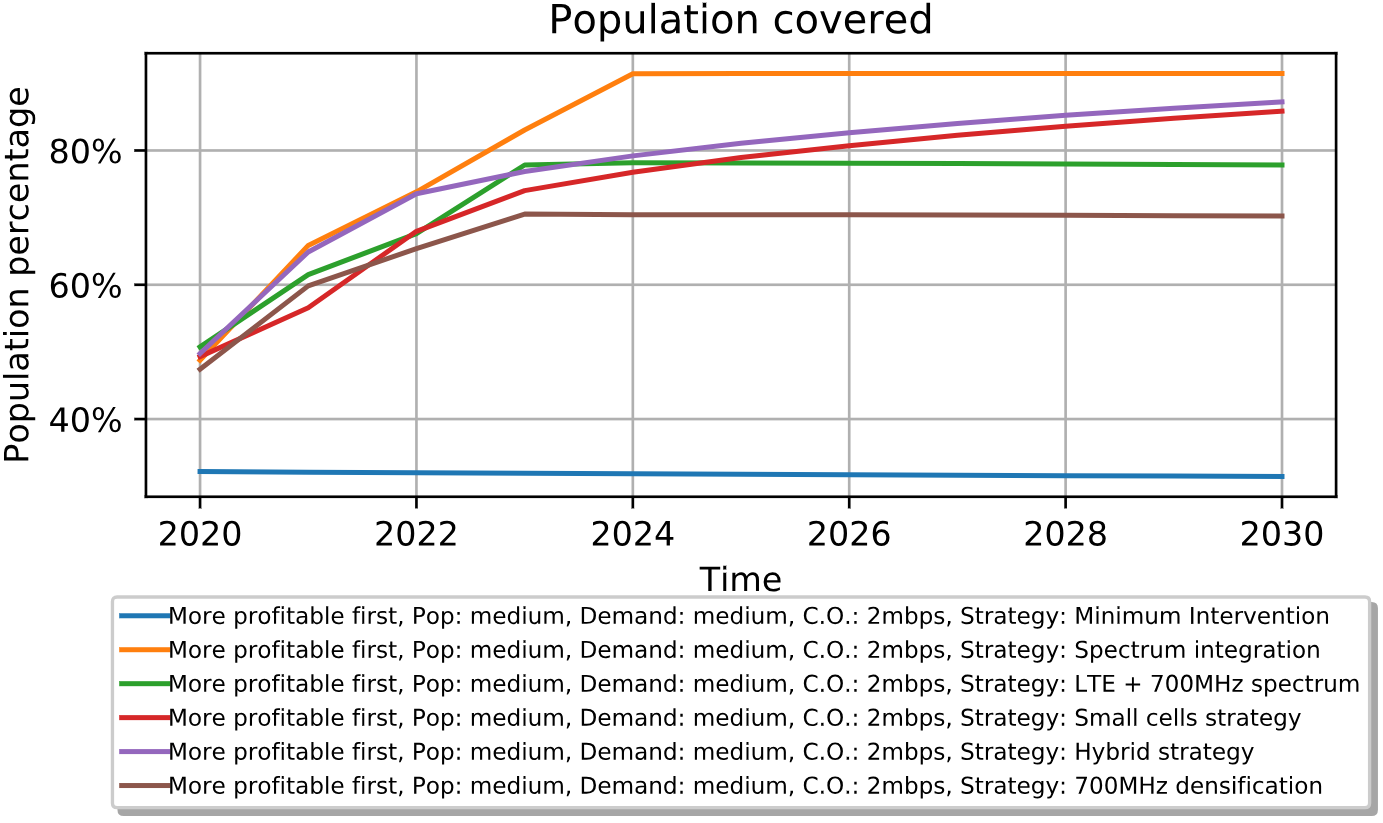
\includegraphics[width=0.95\textwidth]{./media/image50.png}
		\caption{Capacity strategies comparison. Graph: Population covered. Source: Author}
	\end{Center}
\end{figure}


%%%%%%%%%%%%%%%%%%%% Figure/Image No: 11 Ends here %%%%%%%%%%%%%%%%%%%%

This graph represents the population covered after the interventions of any one year. This way, the starting percentage is 32$\%$  and is the same for all the interventions. As can be seen in the plot, not all the lines reach 100$\%$  of the population covered by 2030. Apart from �\textit{Minimum intervention�}, that cannot build new assets and, therefore, does not increase the population covered, there are two main groups of strategies: those that can build new assets (\textit{�700 MHz densification�}, \textit{�Small cells strategy� }and \textit{�Hybrid strategy�}) and those that cannot (\textit{�Spectrum integration� }and \textit{�700 MHz spectrum integration �}).\par

In the graph, only \textit{�Small cells strategy� }and \textit{�Hybrid strategy�} could potentially reach the 100$\%$  population covered while the rest only raise the percentage from 32$\%$  to 70-90$\%$ . This is because, while the small cells related strategies increase the percentage of population covered during the whole simulation, the rest stop growing around 2023-24. This is because of two factors: (I) the extremely good capacity of the small cells in the model and (II) that MINERVA allows densification strategies, which means creating more sites for small cells until all the demand is satisfied. If these strategies really achieve the 100$\%$  population covered will be studied later.\par

\textit{�700 MHz densification�} is also allowed to create new sites, but the 700 MHz band has less bandwidth than 3.7 GHz and, therefore, using only this band is not enough to meet the demand in some regions. Finally, the rest of the strategies are not allowed to create new sites, just to upgrade those sites that already have legacy technologies (Such as 2G and 3G). These strategies cannot satisfy the demand either but due to two different factors:\par

\begin{itemize}
	\item Checking the list of assets provided in the original model, there is a part of the PCDs that have no assets at the beginning of the execution in the whole PCD. This is not an issue of the behaviour of the code, but of the database from which this information was obtained for the NISMOD project. Half of the interventions (Except \textit{�Small cells strategy�, �Hybrid strategy� and �700 MHz densification�}) cannot build new assets, and, therefore, strategies that only use this type of interventions are affected by this limitation.\par

	\item The other factor is that there is a limit to the capacity that one band can provide. Strategies that only use one or two bands, such as \textit{�700 MHz spectrum integration �} and \textit{�700 MHz densification�} are mainly affected by this limitation in the most densely populated regions.
\end{itemize}\par

\textit{�Spectrum integration�} strategy grows with the similar rate than the other macrocell related strategies, but when they stop growing, the \textit{�Spectrum integration� }strategy continues the rise a little bit more and manages to reach around the 90$\%$  of the population. This is because it is the only strategy allowed to build assets with the 3,500 MHz band which has the bigger bandwidth and hence provides more capacity.\par

\subsection*{Investment}
%\addcontentsline{toc}{subsection}{Investment}
The second output that we will review is the comparison of costs. The following graph compares the investment effort that the telecom operator would make depending on the capacity expansion strategy. This graph also uses the baseline population growth scenario, the baseline user-speed growth scenario, and the \textit{�More profitable first�} coverage obligation option with a speed of 2 Mbps.\par


%%%%%%%%%%%%%%%%%%%% Figure/Image No: 12 starts here %%%%%%%%%%%%%%%%%%%%

\begin{figure}[H]
	\begin{Center}
		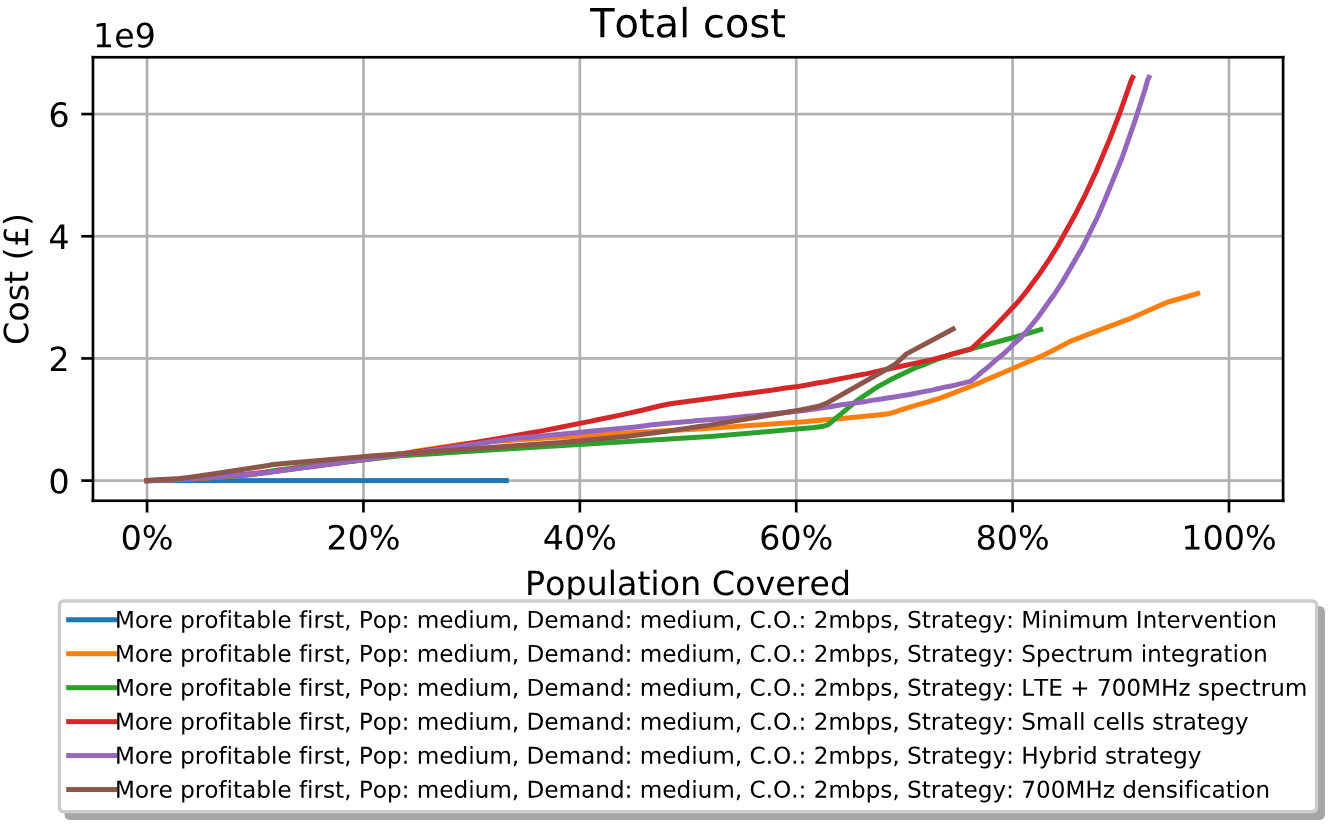
\includegraphics[width=0.95\textwidth]{./media/image51.png}
		\caption{Capacity strategies comparison. Graph: Total cost. Source: Author}
	\end{Center}
\end{figure}


%%%%%%%%%%%%%%%%%%%% Figure/Image No: 12 Ends here %%%%%%%%%%%%%%%%%%%%

The given graph represents the cost that takes to reach a specific population covered percentage for each capacity strategy. As can be seen in the plot, none of the lines reaches 100$\%$  since they cannot cover the whole population by 2030.\par

From the beginning to 75$\%$  covered, which are the urban and suburban areas, the marginal cost to increase by 1$\%$  is similar for most of the strategies. The $``$Small cells$"$  strategy is a little bit more expensive since it starts building small cells directly, while the rest of strategies use LTE or 700 MHz bands before. After 75$\%$  of the population, the cost of both small cells strategies grows drastically and makes it not affordable.\par

The graph also reflects the differences between all the strategies that only use macrocell bands (700, 800, 2,600, 3,500 MHz). \textit{�Spectrum integration�} is the best strategy since can use all the bands and the only one that can use the 3,500 MHz band. Hence, the gap from 85$\%$  of the population covered to 95$\%$  is just thanks to adding this band, which helps in those regions where the rest of the bands combined were not enough. \textit{�700 MHz spectrum integration� }has LTE and 700 MHz, while \textit{�700 MHz densification�} only uses the 700 MHz. For this reason, despite \textit{�700 MHz densification�} can create new sites and can provide connectivity in places where it is not possible with the other strategies, \textit{�700 MHz spectrum integration� }is capable of covering much more population at the end of the execution. It is important to remember that these strategies are not limited by the budget of the operator, but by the technical issues explained above.\par


\subsection*{Capacity margin}
%\addcontentsline{toc}{subsubsection}{Capacity margin}
The capacity margin is the third and last output that we are going to evaluate, and it is related to the difference between the absolute value of the capacity of the network and the absolute value of the demand of the network in Mbps/km\textsuperscript{2}. This is not related to the coverage obligations, but to the estimated demand of the population. The following graph uses the baseline population growth scenario, the baseline user-speed growth scenario, and the \textit{�More profitable first�} coverage obligation option with a speed of 2 Mbps.\par



%%%%%%%%%%%%%%%%%%%% Figure/Image No: 13 starts here %%%%%%%%%%%%%%%%%%%%

\begin{figure}[H]
	\begin{Center}
		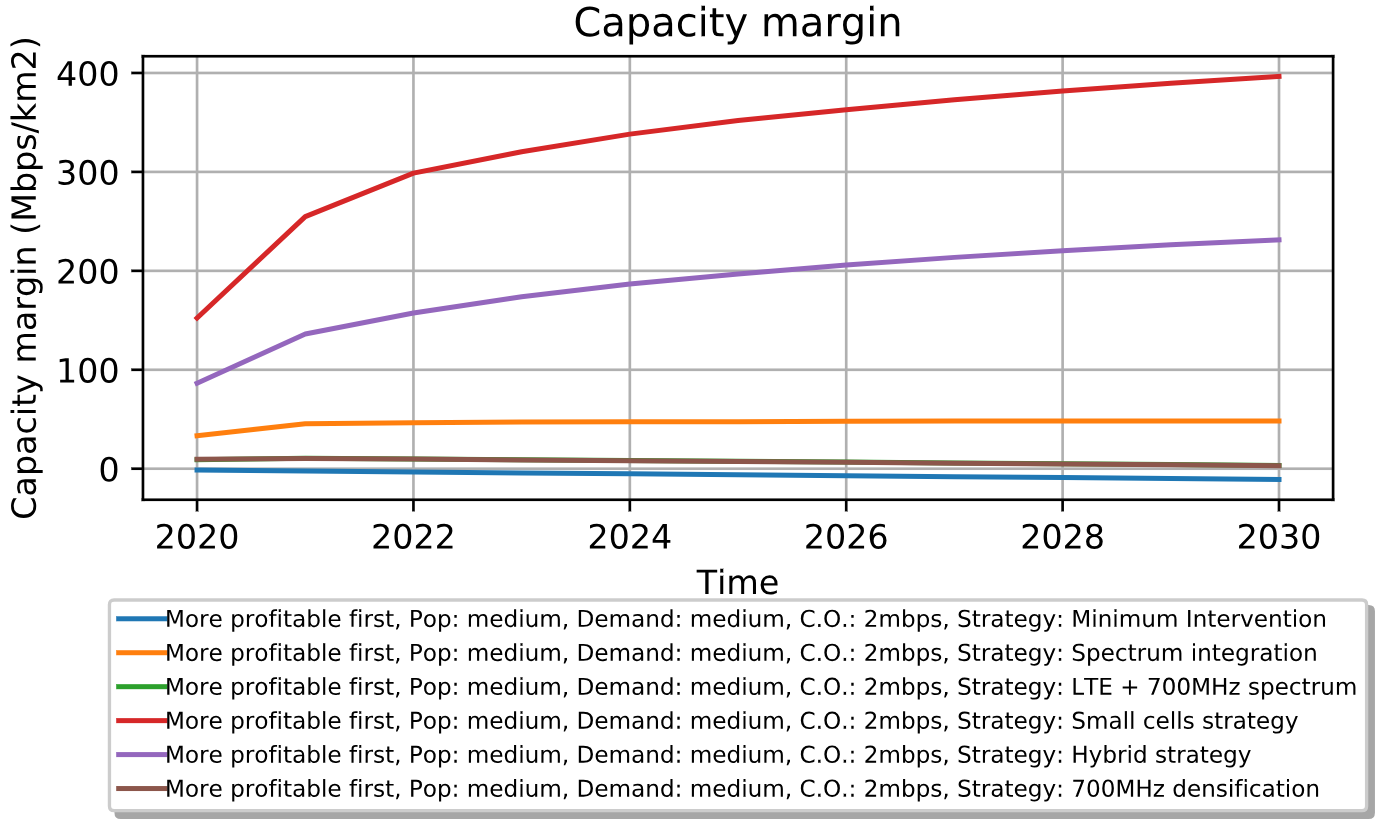
\includegraphics[width=0.95\textwidth]{./media/image52.png}
		\caption{Capacity strategies comparison. Graph: Capacity margin. Source: Author}
	\end{Center}
\end{figure}


%%%%%%%%%%%%%%%%%%%% Figure/Image No: 13 Ends here %%%%%%%%%%%%%%%%%%%%

The most interesting strategy for a telecom operator is to have high population covered, with the minimum cost possible and with a positive capacity margin but as small as possible. Otherwise, it would mean that the operator made a big investment that is not been harnessed. \par

This graph shows the same differences that we could see before. There is a strong difference between strategies that use the small cells intervention and those that do not. Small cells are good but expensive and using just small cells comprise a huge waste of budget in the less populated areas.\par

\subsection*{Total costs }
%\addcontentsline{toc}{subsection}{Total costs }
The model calculates that a telecom operator with a market share of 30$\%$  of the population that use mobile broadband services have approximately �600,000,000 per year to invest in new assets and operate them. The purpose of this section is to verify which of the limitations that we found in the previous charts are due to technical or monetary restrictions. In the case of the limitations that were because of the budget, this model also shows the total amount of money that would be needed.\par

The following chart represents the same information as the cost section, which is the cost that takes to achieve certain population covered, but removing the budget limitations:\par



%%%%%%%%%%%%%%%%%%%% Figure/Image No: 14 starts here %%%%%%%%%%%%%%%%%%%%

\begin{figure}[H]
	\begin{Center}
		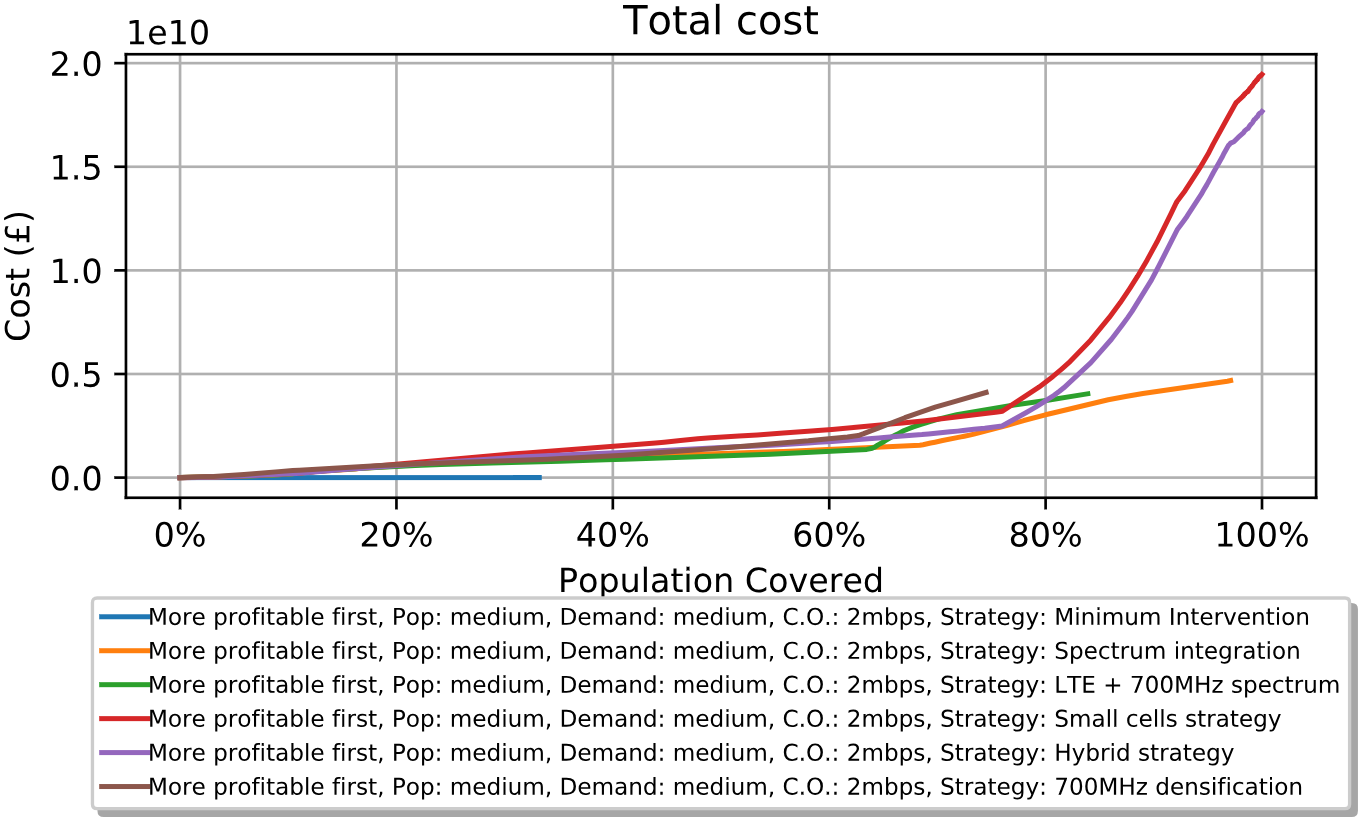
\includegraphics[width=0.95\textwidth]{./media/image53.png}
		\caption{Capacity strategies comparison. Graph: Total cost without budget limitation. Source: Author}
	\end{Center}
\end{figure}


%%%%%%%%%%%%%%%%%%%% Figure/Image No: 14 Ends here %%%%%%%%%%%%%%%%%%%%

As can be seen, the graph is similar to the previous one, but now the \textit{�Small cells strategy�} and the \textit{�Hybrid strategy�} strategies reach the 100$\%$  population covered, which confirms the previous analysis. \par

The maximum budget that the operator can spend in 11 years (From 2020 to 2030) is �6,600,000,000 which was the maximum value of the Y-axis in the budget limited cost chart. Now, the total cost is �20,600,000,000 which is three times the budget that the operator has. In fact, it is also important to remark that rising the population covered from 90$\%$  to 100$\%$  implies spending more than two times of what it took to rise from the original coverage to 90$\%$ .\par

The rest of strategies are not modified since they were not limited by budget but by technical constraints.\par

The capacity margin is also affected in this case and the results are not good for the small cells since the final capacity margin is too big. The following graph represents the capacity margin per year. As the budget is not limited, the operator builds all the assets in 2020, but it shows the differences between strategies clearly. \par



%%%%%%%%%%%%%%%%%%%% Figure/Image No: 15 starts here %%%%%%%%%%%%%%%%%%%%

\begin{figure}[H]
	\begin{Center}
		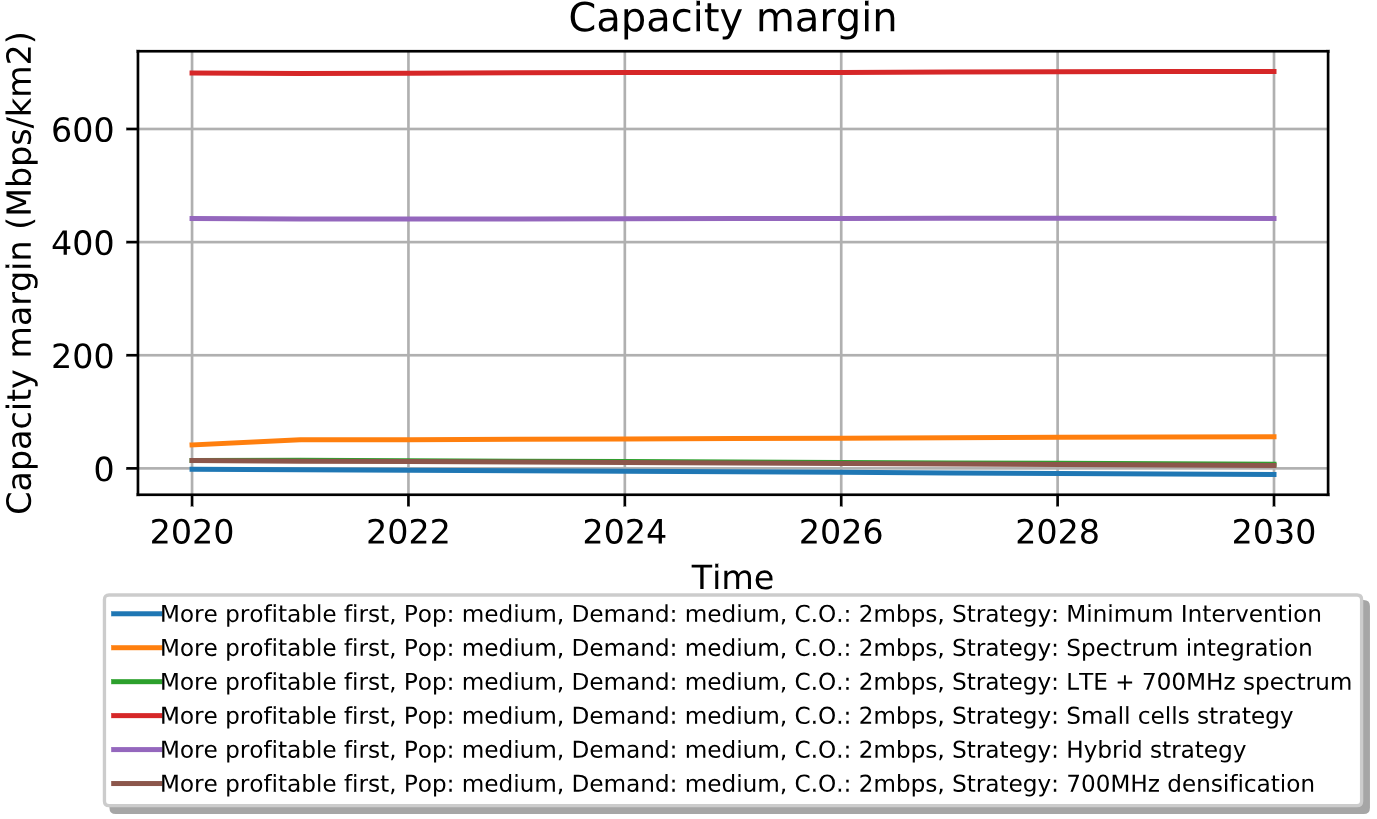
\includegraphics[width=0.95\textwidth]{./media/image54.png}
		\caption{Capacity strategies comparison. Graph: Capacity margin without budget limitation. Source: Author}
	\end{Center}
\end{figure}


%%%%%%%%%%%%%%%%%%%% Figure/Image No: 15 Ends here %%%%%%%%%%%%%%%%%%%%

The important point of this graph is that it allows us to see which is the maximum capacity margin for each capacity expansion strategy. In the previous capacity margin graph, the small cells related strategies did not stop growing their margin. In this graph, we can see the real final value of the strategies. However, the rest of the strategies do not increase their margin in spite of having an unlimited budget. This is mainly because these strategies have a technical limitation, not a budget limitation. \par


\section{Coverage obligation sets}
%\subsection*{Coverage obligation options}
%\addcontentsline{toc}{section}{Coverage obligation sets}
In this section, a detailed study of the coverage obligation sets will be provided. The aim is to be able to understand the implications that each of them has in the development of the new mobile broadband assets deployment in the country. In the previous chapter, we analysed the �\textit{More profitable first�} option, which is the original version. Now, four new sets are analysed: �\textit{Priority areas first�, �Less profitable areas first�, �Only rural areas� and �Nation-balanced�.} Finally, we will compare them using two types of capacity expansion strategies to assess the advantages and disadvantages of each of them.\par

\subsection{Priority areas first}
This is the first of the coverage obligation sets and divides all the PCDs into two sections: First, it invests in the 18$\%$  less densely populated PCDs, starting in the most densely populated of those and later it invests in the rest of them, starting in the most densely populated of this subgroup. It is explained in higher detail in the previous chapter. We are going to analyse how it behaves using two different capacity expansion strategies: (I) \textit{�Hybrid strategy�}, which makes use of all the possible interventions, and (II) \textit{�700 MHz densification�}, which is the strategy that I have designed in this thesis.\par

\subsubsection*{�Hybrid strategy�}
%\addcontentsline{toc}{subsubsection}{�Hybrid strategy�}
The first graph that we are going to analyse is the cost that takes to increment the population covered. As \textit{�Priority areas first�} starts in with the 18$\%$  less densely populated and, therefore, less profitable, the graph has a different shape than the one that had with \textit{�Most profitable first�:}\par



%%%%%%%%%%%%%%%%%%%% Figure/Image No: 1 starts here %%%%%%%%%%%%%%%%%%%%

\begin{figure}[H]
	\begin{Center}
		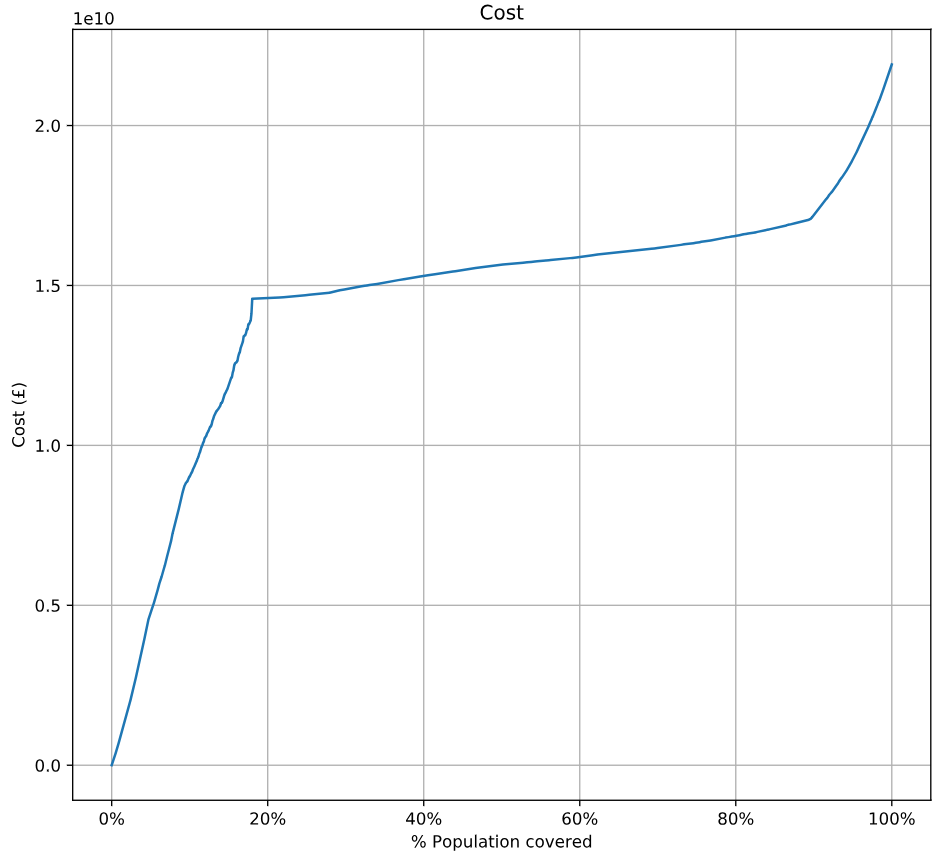
\includegraphics[width=1\textwidth]{./media/image55.png}
		\caption{Priority areas first - Hybrid strategy. Graph: Cost. Source: Author}
	\end{Center}
\end{figure}


%%%%%%%%%%%%%%%%%%%% Figure/Image No: 1 Ends here %%%%%%%%%%%%%%%%%%%%

First, we have to cover the most rural areas and, therefore, the curve is so steep. After the 18$\%$  population is covered, the slope of the curve gets reduced immediately, because we start to cover the most densely populated. When it reaches the 90$\%$  of the population, the marginal cost escalates because we change to the rural geotype again, which have worse propagation properties.\par

This combination of coverage obligation set and capacity strategy has two main disadvantages: (i) it forces the operator to invest in all of the PCDs, but starting in the less-profitable 18$\%$  and (ii) the only option for those PCDs that have no assets deployed at the beginning is to create a full small cells network, which has an exorbitant cost. The result is that the percentage of population covered raises just a little, despite the operator invests all it can for eleven years:\par



%%%%%%%%%%%%%%%%%%%% Figure/Image No: 2 starts here %%%%%%%%%%%%%%%%%%%%

\begin{figure}[H]
	\begin{Center}
		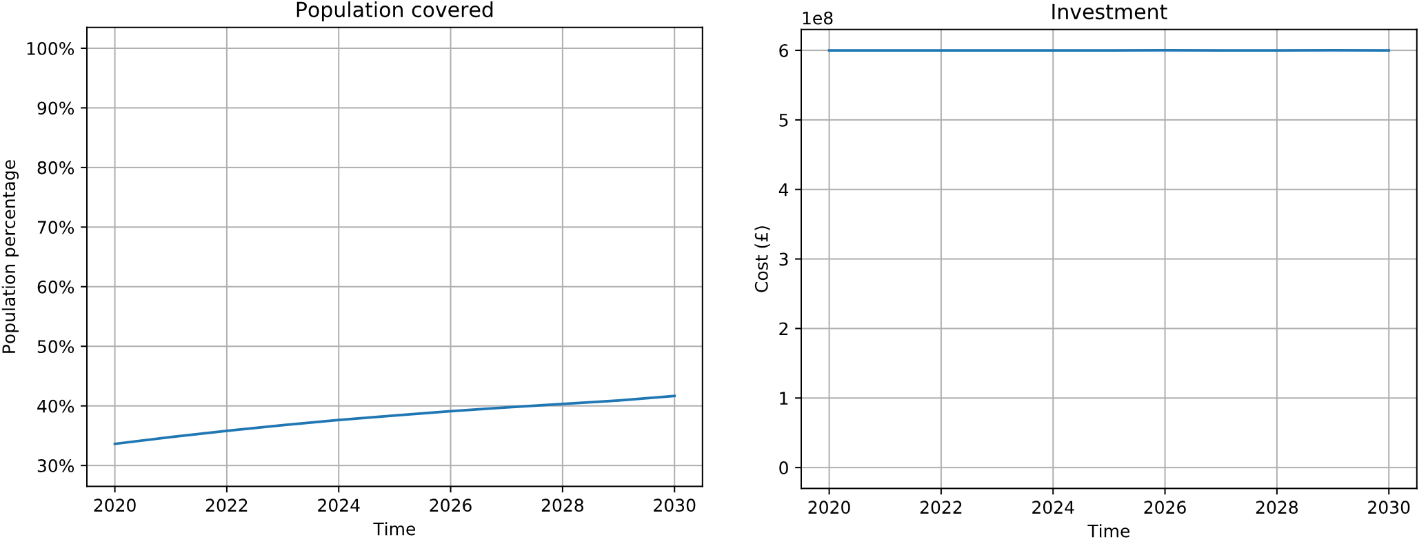
\includegraphics[width=0.95\textwidth]{./media/image56.png}
		\caption{Priority areas first - Hybrid strategy. Graph: Population covered (left) and investment (right). Source: Author}
	\end{Center}
\end{figure}


%%%%%%%%%%%%%%%%%%%% Figure/Image No: 2 Ends here %%%%%%%%%%%%%%%%%%%%

The evolution of the capacity margin over the years is also an important output when it is combined with the investment effort. If the investment effort is huge, as it is here, the capacity margin should raise, reflecting it. In this case, it does not happen since the effort is done in the least profitable areas. The following chart represents how little this output grows nationwide:\par



%%%%%%%%%%%%%%%%%%%% Figure/Image No: 3 starts here %%%%%%%%%%%%%%%%%%%%

\begin{figure}[H]
	\begin{Center}
		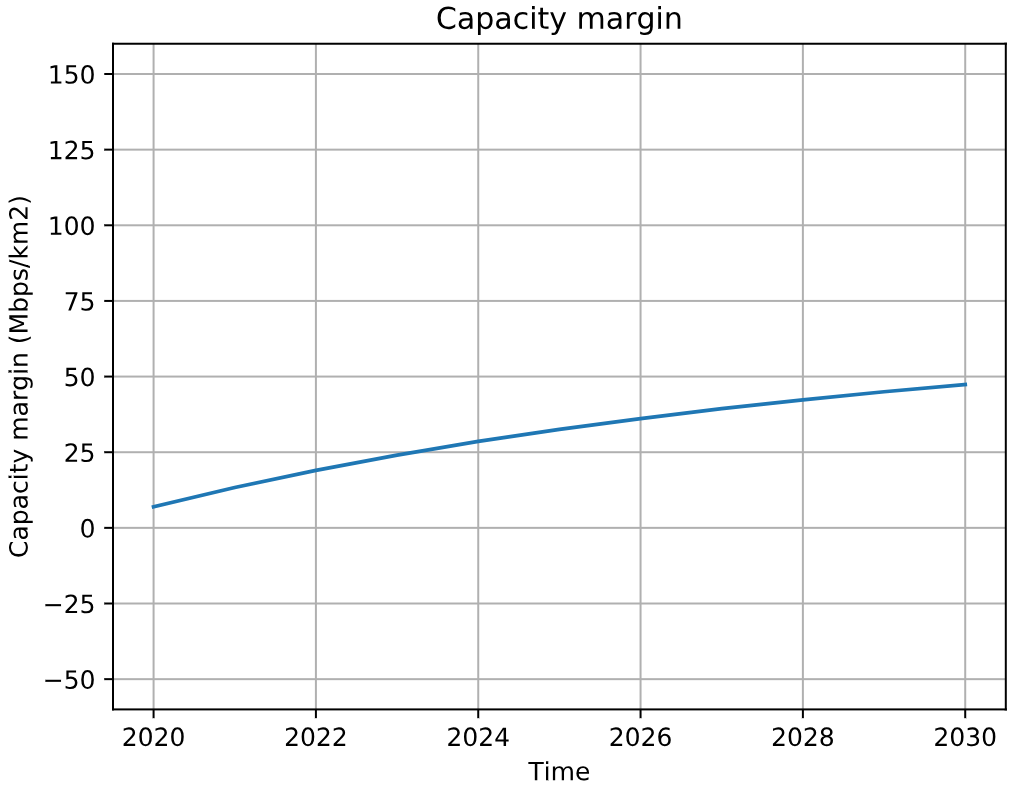
\includegraphics[width=0.70\textwidth]{./media/image57.png}
		\caption{Priority areas first - Hybrid strategy. Graph: Capacity margin. Source: Author}
	\end{Center}
\end{figure}


%%%%%%%%%%%%%%%%%%%% Figure/Image No: 3 Ends here %%%%%%%%%%%%%%%%%%%%


The problem of the previous graph is that it aggregates the capacity margin of all the areas and it does not help us to see the differences between areas. The following two histograms represent the probability of a specific capacity margin and its cumulative distribution function, which represent the probability of having at least a specific margin in each PCD: \par



%%%%%%%%%%%%%%%%%%%% Figure/Image No: 4 starts here %%%%%%%%%%%%%%%%%%%%

\begin{figure}[H]
	\begin{Center}
		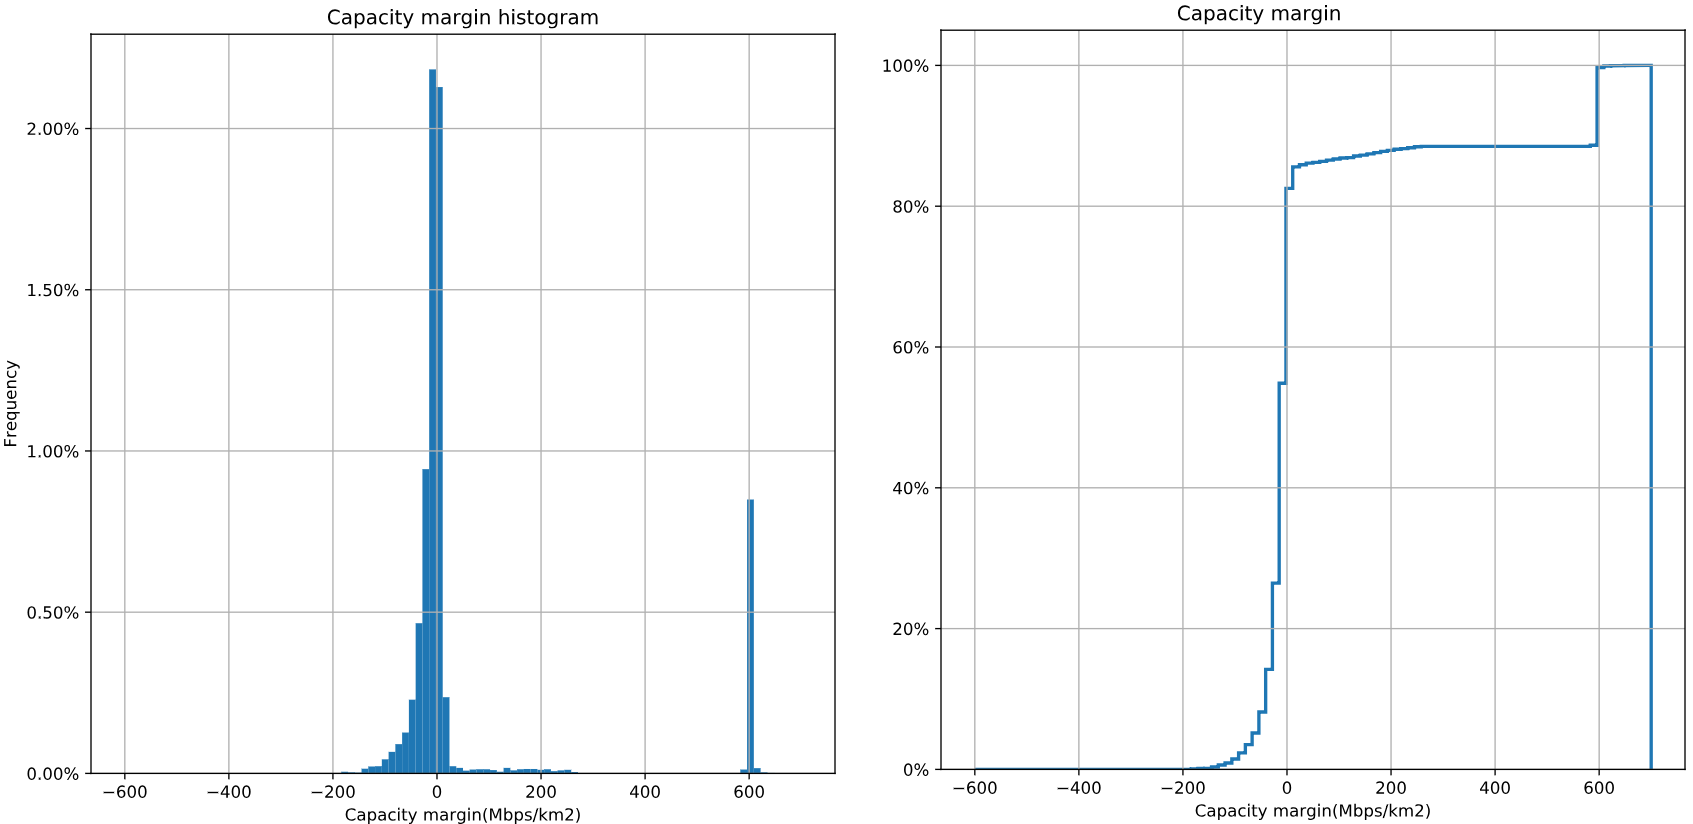
\includegraphics[width=0.95\textwidth]{./media/image58.png}
		\caption{Priority areas first - Hybrid strategy. Histogram: Capacity margin (left) and CDF (right). Source: Author}
	\end{Center}
\end{figure}


%%%%%%%%%%%%%%%%%%%% Figure/Image No: 4 Ends here %%%%%%%%%%%%%%%%%%%%

As it can be seen in the graph, the distribution function of the capacity margin has two main parts: (I) A Gaussian with the mean in 0 and low variance and (II) a group of PCDs whose capacity margin is around 600 Mbps/km2. This is a clear indicator of the low suitability of this combination since, instead of gradually giving more capacity to all the PCDs, it gives a huge capacity to only some of them, creating two distinct groups.\par

The distribution of the percentage of population covered along the PCDs is another value that we are going to consider, and we will see that its distribution is quite similar to the capacity margin one. \par



%%%%%%%%%%%%%%%%%%%% Figure/Image No: 5 starts here %%%%%%%%%%%%%%%%%%%%

\begin{figure}[H]
	\begin{Center}
		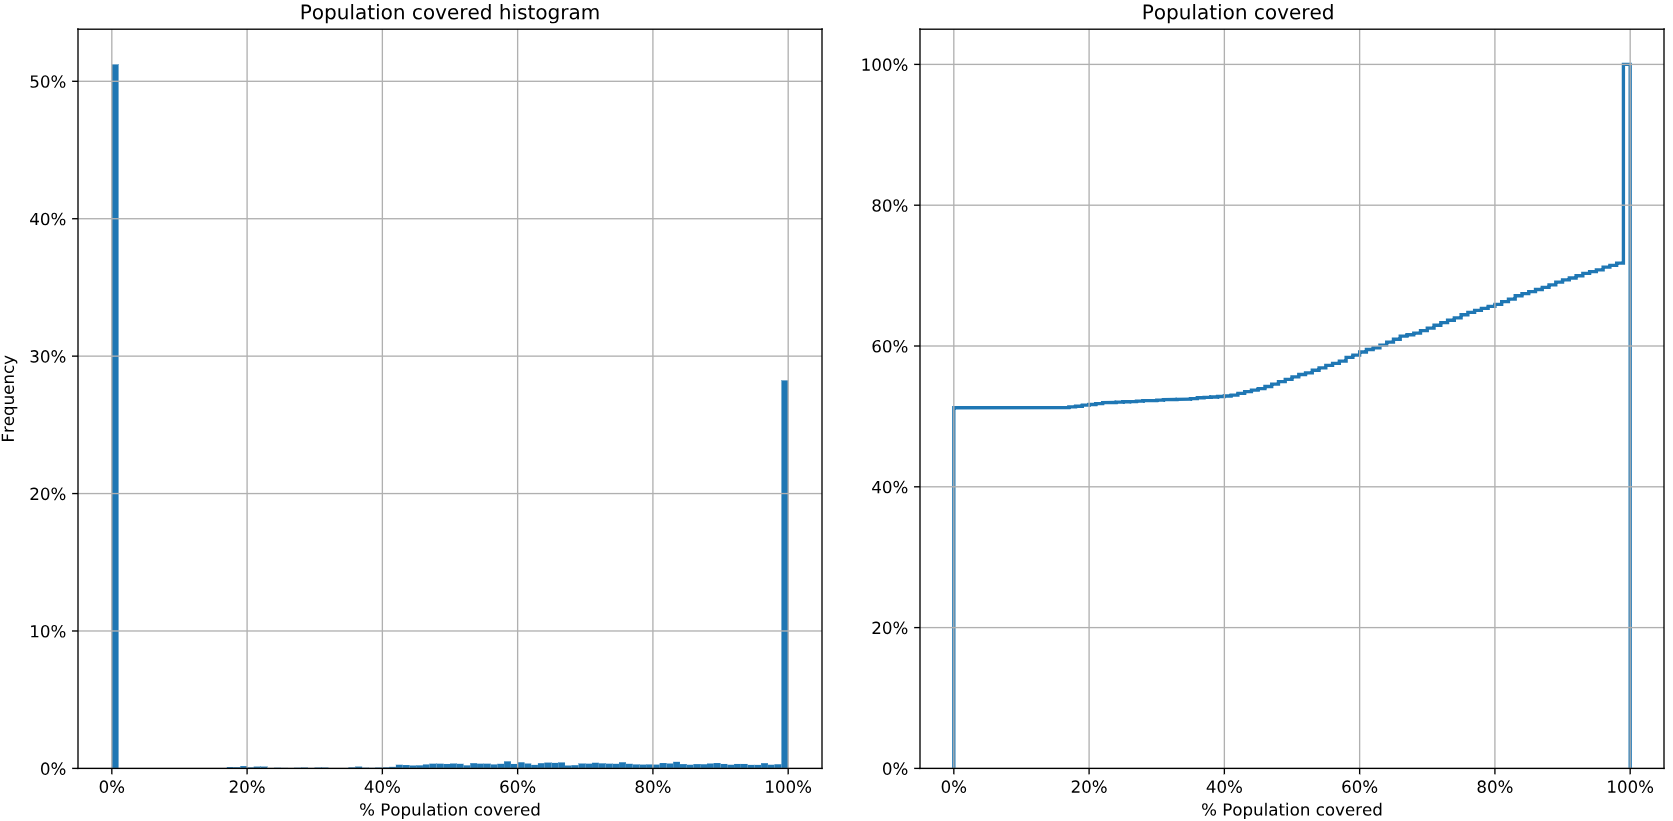
\includegraphics[width=0.95\textwidth]{./media/image59.png}
		\caption{Priority areas first - Hybrid strategy. Histogram: Population covered (left) and CDF (right). Source: Author}
	\end{Center}
\end{figure}


%%%%%%%%%%%%%%%%%%%% Figure/Image No: 5 Ends here %%%%%%%%%%%%%%%%%%%%

The problem with the population covered is that, as we spend a lot of resources in the priority areas, there is no more budget for the more profitable ones. Fifty per cent of the PCDs has 0$\%$  population covered since no money is invested there. Almost 30$\%$  of the areas have more than the capacity needed and are covered at 100$\%$  and the rest have an intermediate capacity thanks to the assets that they had already built before the execution of the simulation.\par

Now, we are going to evaluate these parameters using some coloured maps, so we can see exactly the differences between regions in the UK map. First, we are going to see the investment per year and LAD. It is important to notice that the most densely populated regions never receive investments, while the money is spent only in some regions.\par



%%%%%%%%%%%%%%%%%%%% Figure/Image No: 6 starts here %%%%%%%%%%%%%%%%%%%%

\begin{figure}[H]
	\begin{Center}
		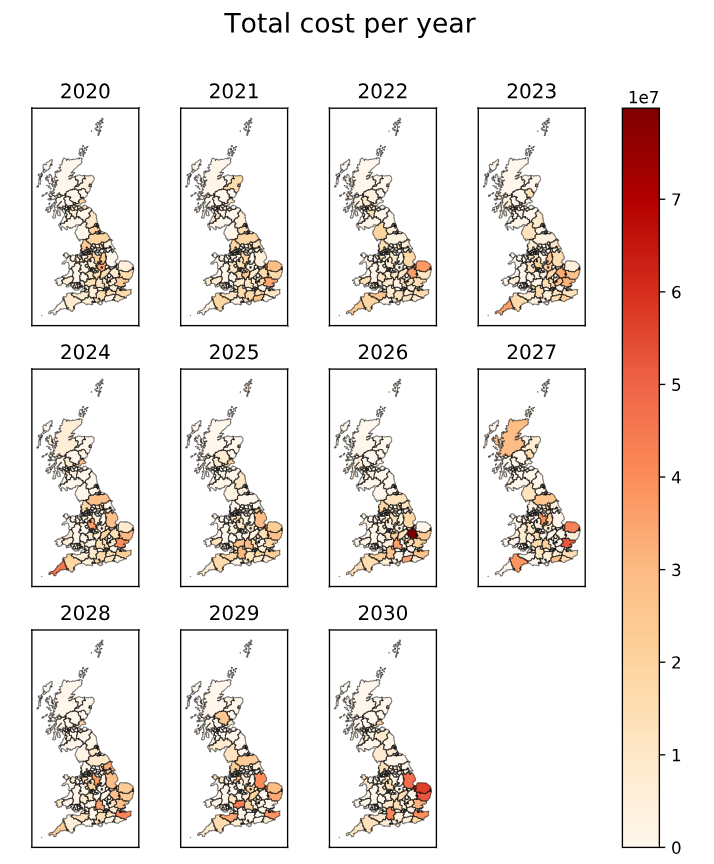
\includegraphics[width=0.85\textwidth]{./media/image60.png}
		\caption{Priority areas first - Hybrid strategy. Map: Cost. Source: Author}
	\end{Center}
\end{figure}


%%%%%%%%%%%%%%%%%%%% Figure/Image No: 6 Ends here %%%%%%%%%%%%%%%%%%%%


This distribution of the investment has an impact on two metrics: the population covered and the capacity margin. These maps represent the evolution of those over the years. As it can be seen in the capacity margin maps, it gets too high in some regions (200Mbps/km\textsuperscript{2} in some cases), while it remains as it was at the beginning in the ones that have more population.\par



%%%%%%%%%%%%%%%%%%%% Figure/Image No: 7 starts here %%%%%%%%%%%%%%%%%%%%

\begin{figure}[H]
	\begin{Center}
		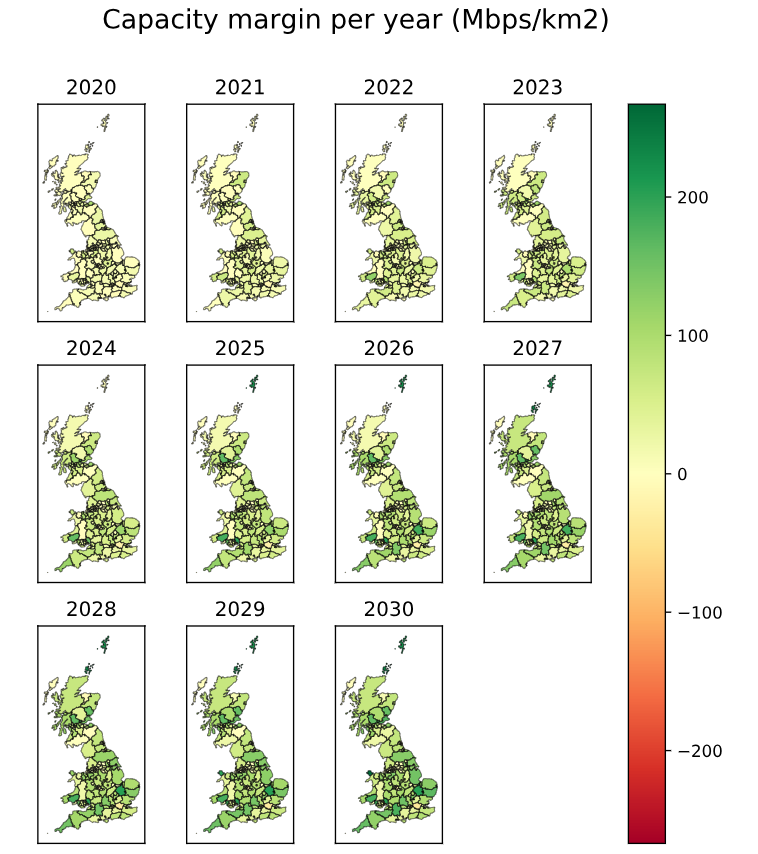
\includegraphics[width=0.95\textwidth]{./media/image61.png}
		\caption{Priority areas first - Hybrid strategy. Map: Capacity margin. Source: Author}
	\end{Center}
\end{figure}


%%%%%%%%%%%%%%%%%%%% Figure/Image No: 7 Ends here %%%%%%%%%%%%%%%%%%%%

The following map represents the evolution of the population covered parameter. As it can be seen, this output improves over the course of time, but not with the same growth rate that other capacity expansion strategies have.\par


%%%%%%%%%%%%%%%%%%%% Figure/Image No: 8 starts here %%%%%%%%%%%%%%%%%%%%

\begin{figure}[H]
	\begin{Center}
		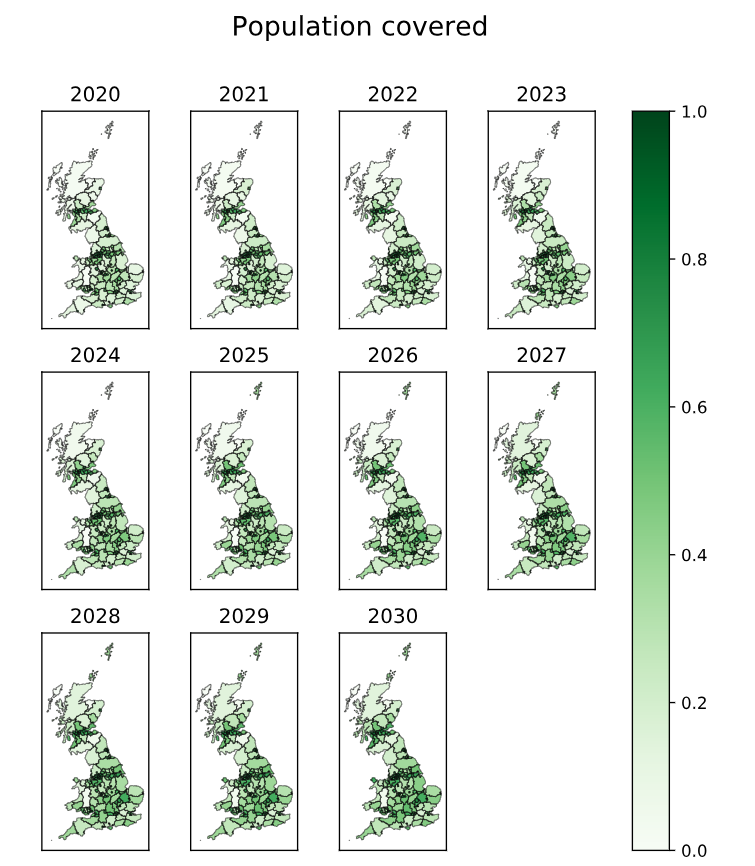
\includegraphics[width=1\textwidth]{./media/image62.png}
		\caption{Priority areas first - Hybrid strategy. Map: Population covered. Source: Author}
	\end{Center}
\end{figure}


%%%%%%%%%%%%%%%%%%%% Figure/Image No: 8 Ends here %%%%%%%%%%%%%%%%%%%%


\paragraph*{No budget limitation}
%\addcontentsline{toc}{paragraph}{No budget limitation}
Using the same strategy than above, but removing the budget limitation allows us to see how much it would really cost to cover all the population with the obligation and to satisfy the end-user speed demand. The following graph represents the marginal cost that increasing the percentage of population covered implies:\par



%%%%%%%%%%%%%%%%%%%% Figure/Image No: 9 starts here %%%%%%%%%%%%%%%%%%%%

\begin{figure}[H]
	\begin{Center}
		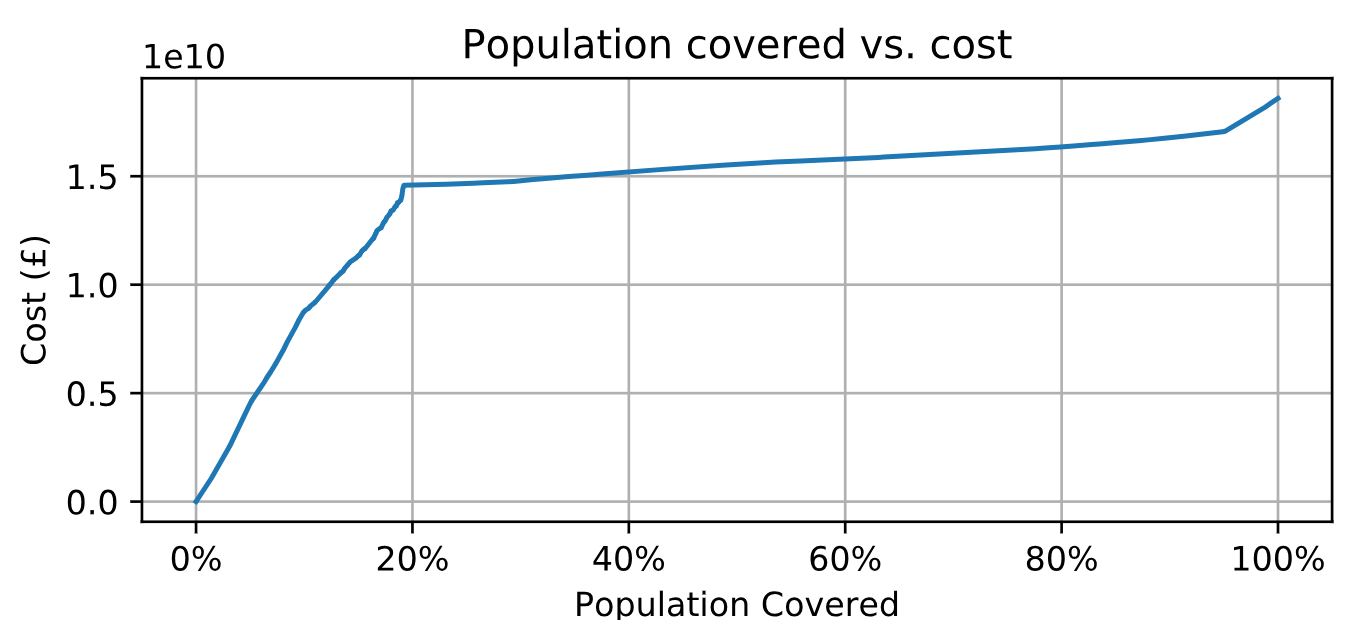
\includegraphics[width=0.7\textwidth]{./media/image63.png}
		\caption{Priority areas first - Hybrid strategy. Graph: Cost without budget limitation. Source: Author}
	\end{Center}
\end{figure}


%%%%%%%%%%%%%%%%%%%% Figure/Image No: 9 Ends here %%%%%%%%%%%%%%%%%%%%


This graph shows that reaching the 100$\%$  is possible using this combination, but the problem is that at the beginning it makes a strong effort in developing regions that are not so profitable. The total costs are around 3 times more than the budget of the telecom operator and, with the real budget, it would only reach the 42$\%$ .\par

\subsubsection*{�700 MHz densification� }
%\addcontentsline{toc}{subsubsection}{�700 MHz densification� }
Now, we are going to test how good the \textit{�700 MHz densification�} strategy works in conjunction with the �\textit{Priority areas first�} coverage obligation set. The major advantage of this strategy is that it can only create assets in the 700 MHz and that the maximum site density of this band is considerably lower than in the case of the small cells. As it can be seen in the following chart, in this case, the investment is not equally during the whole period. \par



%%%%%%%%%%%%%%%%%%%% Figure/Image No: 10 starts here %%%%%%%%%%%%%%%%%%%%

\begin{figure}[H]
	\begin{Center}
		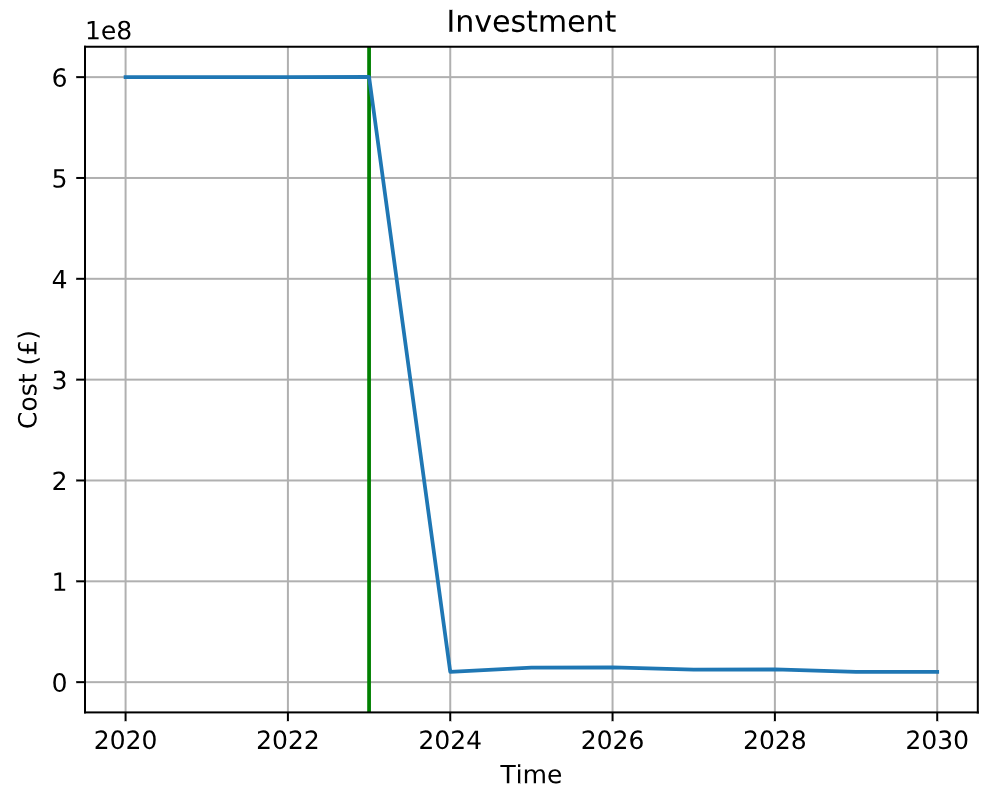
\includegraphics[width=0.55\textwidth]{./media/image64.png}
		\caption{Priority areas first - 700 MHz densification. Graph: Investment. Source: Author}
	\end{Center}
\end{figure}


%%%%%%%%%%%%%%%%%%%% Figure/Image No: 10 Ends here %%%%%%%%%%%%%%%%%%%%


This strategy meets the coverage obligations� investment in the fourth year and after that, it only needs to invest to satisfy the end-user speed demand. However, this graph cannot be understood without analysing the evolution of the capacity margin and population covered. The following graphs represent these values aggregated by year:\par



%%%%%%%%%%%%%%%%%%%% Figure/Image No: 11 starts here %%%%%%%%%%%%%%%%%%%%

\begin{figure}[H]
	\begin{Center}
		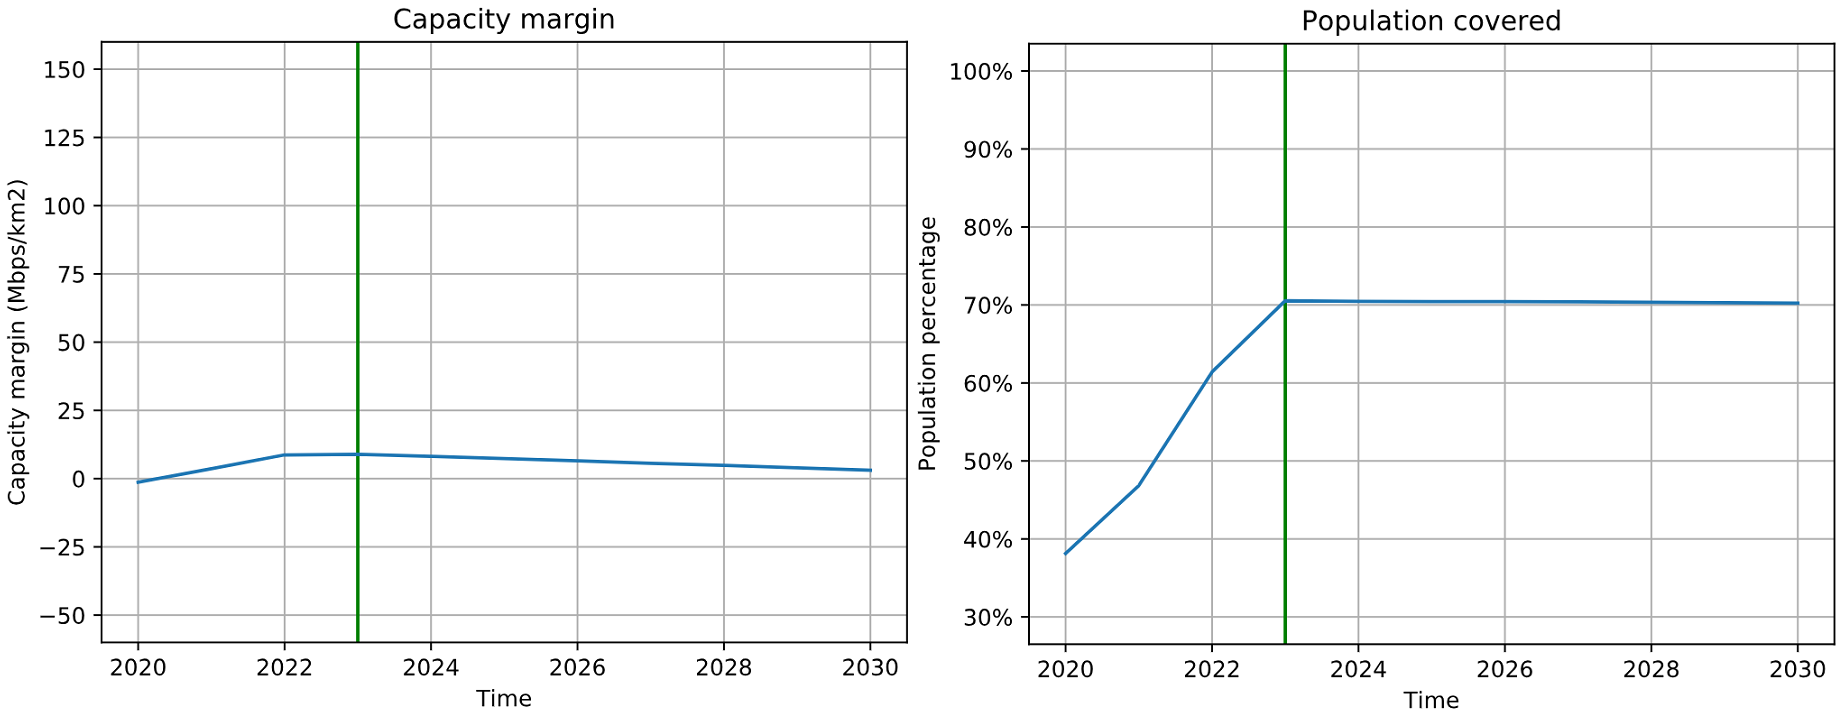
\includegraphics[width=0.9\textwidth]{./media/image65.png}
		\caption{Priority areas first - 700 MHz densification. Graph: Capacity margin (left) and population covered (right). Source: Author}
	\end{Center}
\end{figure}


%%%%%%%%%%%%%%%%%%%% Figure/Image No: 11 Ends here %%%%%%%%%%%%%%%%%%%%

Both outputs show better values than with the �\textit{Hybrid strategy�} strategy since, using less budget, the capacity margin does not growth so much. This means that all the investment effort is done in those areas that need it, but the population covered percentage grows faster and further than in the previous case. The following histograms also show the distribution of the capacity and the percentage of the population covered across the country. The graph on the left shows the CDF of the capacity margin histogram and the one on the right is the histogram of the population covered.\par



%%%%%%%%%%%%%%%%%%%% Figure/Image No: 12 starts here %%%%%%%%%%%%%%%%%%%%

\begin{figure}[H]
	\begin{Center}
		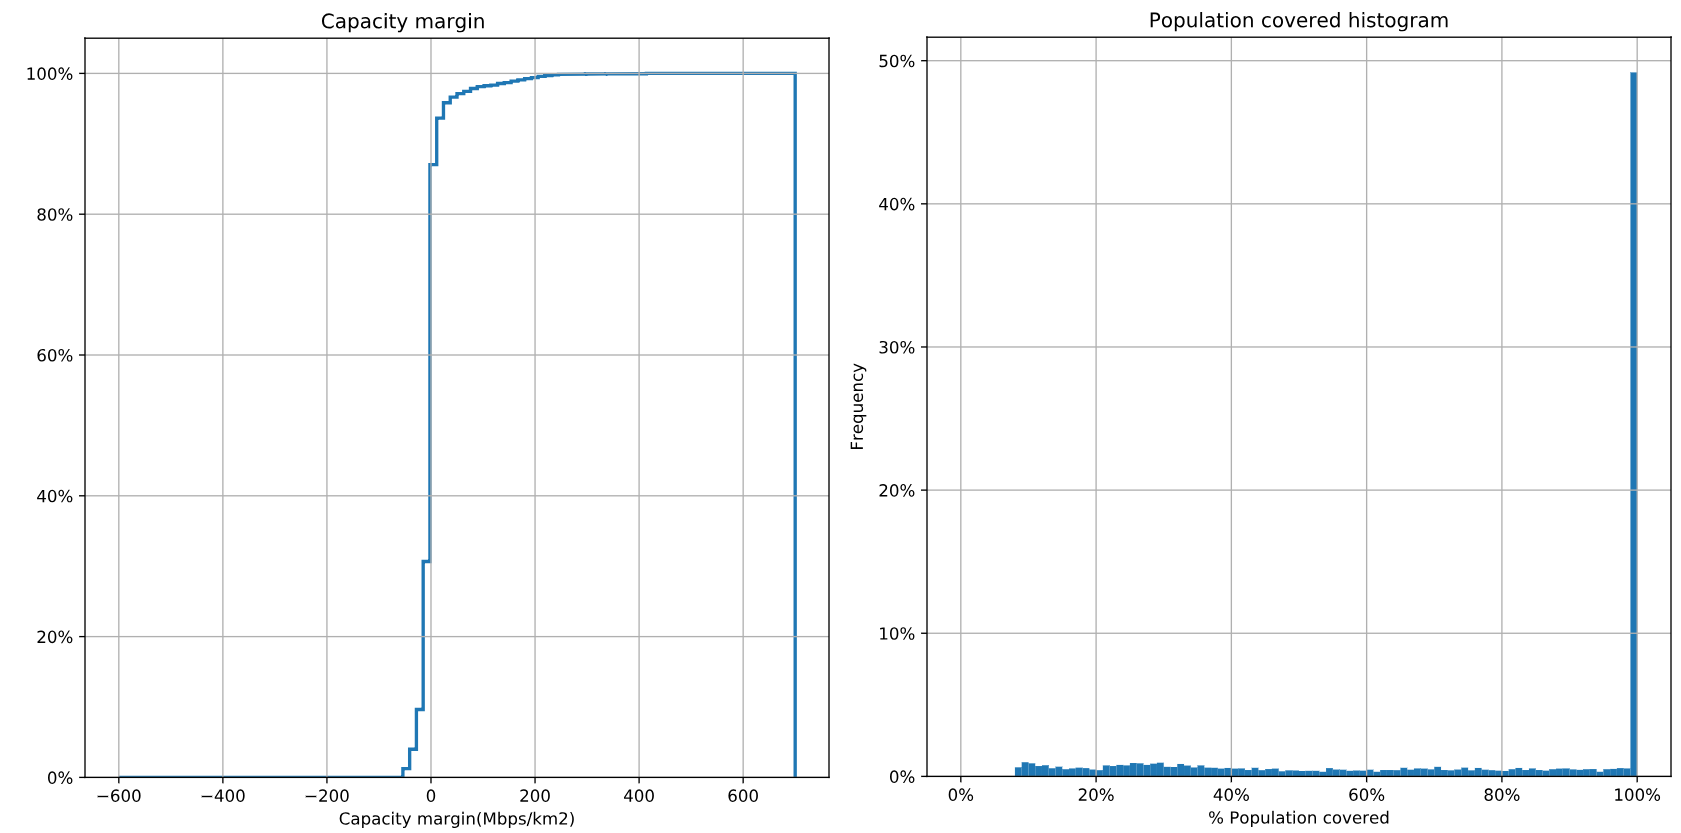
\includegraphics[width=0.9\textwidth]{./media/image66.png}
		\caption{Priority areas first - 700 MHz densification. Graph: Capacity margin CDF (left) and population covered histogram (right). Source: Author}
	\end{Center}
\end{figure}


%%%%%%%%%%%%%%%%%%%% Figure/Image No: 12 Ends here %%%%%%%%%%%%%%%%%%%%


The result is that the capacity margin is mainly around the 0 Mbps/km\textsuperscript{2} which is not a bad result since only 30$\%$  of the PCDs have less margin than 0 Mbps/km\textsuperscript{2} and only 8$\%$  are over it. The population covered histogram represents that all the PCDs received some investment. For half of them, the capacity installed was not enough and require more frequency bands in order to have enough capacity to satisfy the coverage obligation requirements. Despite this, the overall population coverage percentage is really good and most of the PCDs have 100$\%$  or values near to this:\par



%%%%%%%%%%%%%%%%%%%% Figure/Image No: 13 starts here %%%%%%%%%%%%%%%%%%%%

\begin{figure}[H]
	\begin{Center}
		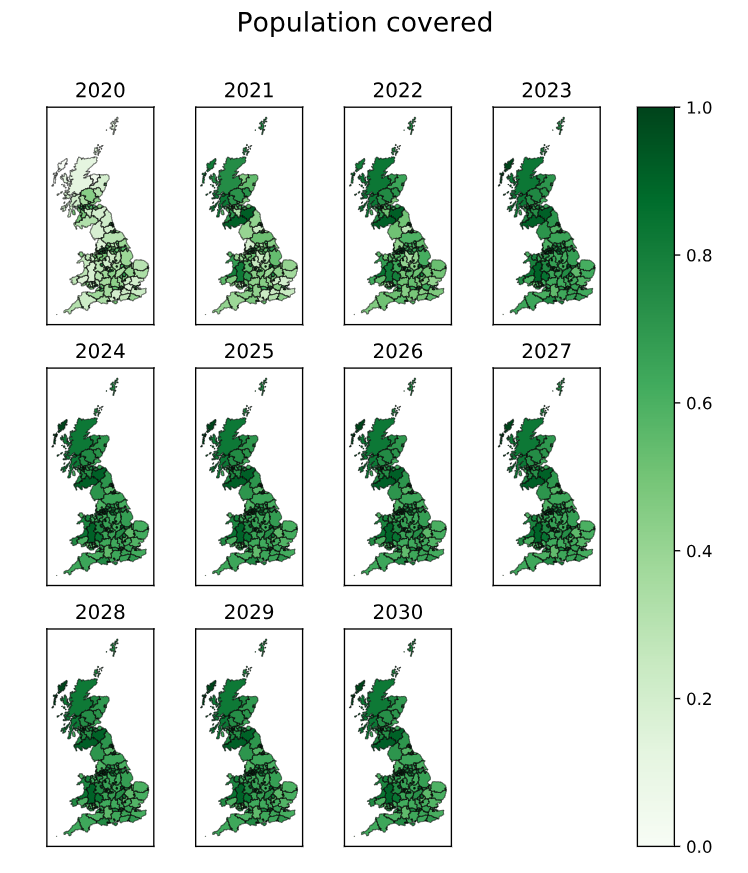
\includegraphics[width=0.95\textwidth]{./media/image67.png}
		\caption{Priority areas first - 700 MHz densification. Map: Population covered. Source: Author}
	\end{Center}
\end{figure}


%%%%%%%%%%%%%%%%%%%% Figure/Image No: 13 Ends here %%%%%%%%%%%%%%%%%%%%


This coloured map is significantly better in terms of coverage than the results of the \textit{�Hybrid strategy�}.\par

Finally, the following graph shows the cost of incrementing the percentage of population covered. It is important to stress that the differences in the results between this graph and the one in section 4.1 are only because of the selected coverage obligation set. In this case, investment starts in some of the less-profitable PCDs and, therefore, the graph starts with a higher slope. Then, after the 18$\%$ , the slope is reduced.\par


%%%%%%%%%%%%%%%%%%%% Figure/Image No: 14 starts here %%%%%%%%%%%%%%%%%%%%

\begin{figure}[H]
	\begin{Center}
		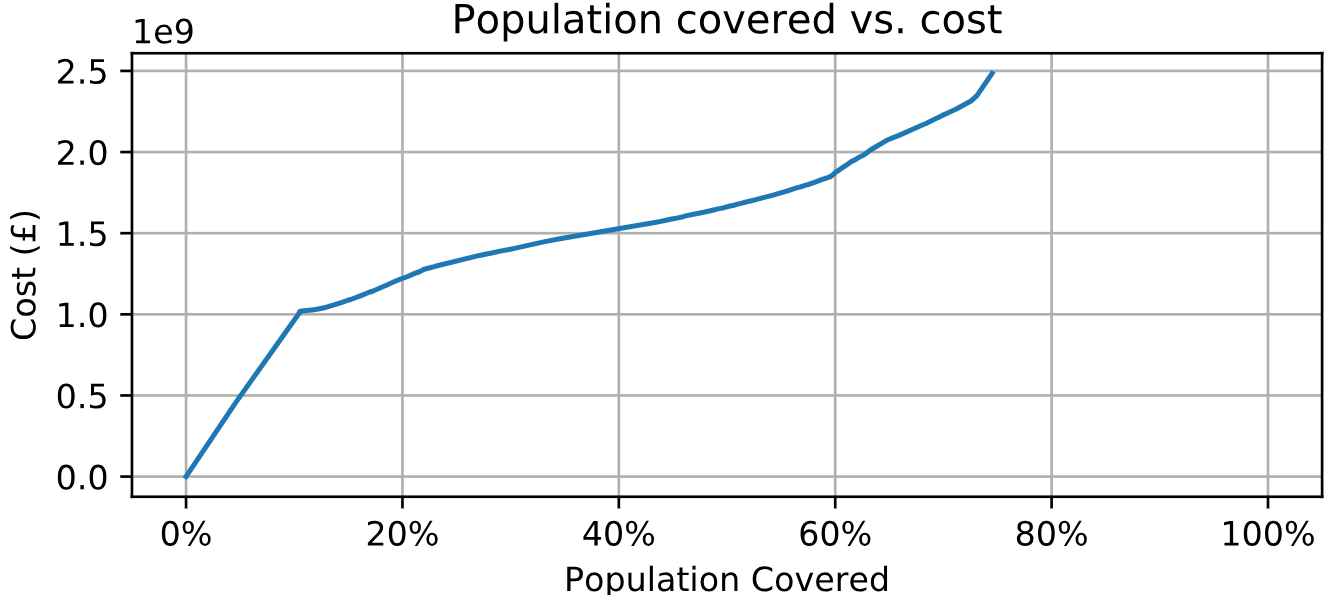
\includegraphics[width=0.75\textwidth]{./media/image68.png}
		\caption{Priority areas first - 700 MHz densification. Graph: Population covered vs. cost. Source: Author}
	\end{Center}
\end{figure}


%%%%%%%%%%%%%%%%%%%% Figure/Image No: 14 Ends here %%%%%%%%%%%%%%%%%%%%


The 700 MHz band is aimed at covering large portions of fields with lower costs and not at providing huge end-user speeds. Hence, this capacity expansion strategy has better results in this situation, where the coverage obligation set starts investing in the less populated areas.\par

\paragraph*{No budget limitation}
\addcontentsline{toc}{paragraph}{No budget limitation}
In this case, there is no difference between having a budget limitation or not since not all the budget is spent even when there is a budget limit. Therefore, almost all the graphs in the previous section also apply to this situation. Obviously, the only graphs that do not match are those that are related to the evolution over the years since, in this case, all the investment is done the first year.\par





















\subsection{Less profitable areas first}
Now, we are going to analyse the second coverage obligation set developed in this study. This strategy allows the telecom operator to build new assets in a PCD only if it has already invested in all of the PCDs with less population density. We are going to test how it behaves for two different capacity expansion strategies: \textit{�Hybrid strategy�} and \textit{�700 MHz densification�.}\par

\subsubsection*{�Hybrid strategy�}
%\addcontentsline{toc}{subsubsection}{�Hybrid strategy�}
Although I am not showing the investment evolution again, the situation is similar as in \textit{�Priority areas first�. }Using the �\textit{Hybrid strategy}� the telecom operator invests to the fullest capacity for all the years and even then, the results are not what was expected. The following graphs represent the evolution of the capacity margin, on the left, and the population covered over the years, on the right:\par



%%%%%%%%%%%%%%%%%%%% Figure/Image No: 15 starts here %%%%%%%%%%%%%%%%%%%%

\begin{figure}[H]
	\begin{Center}
		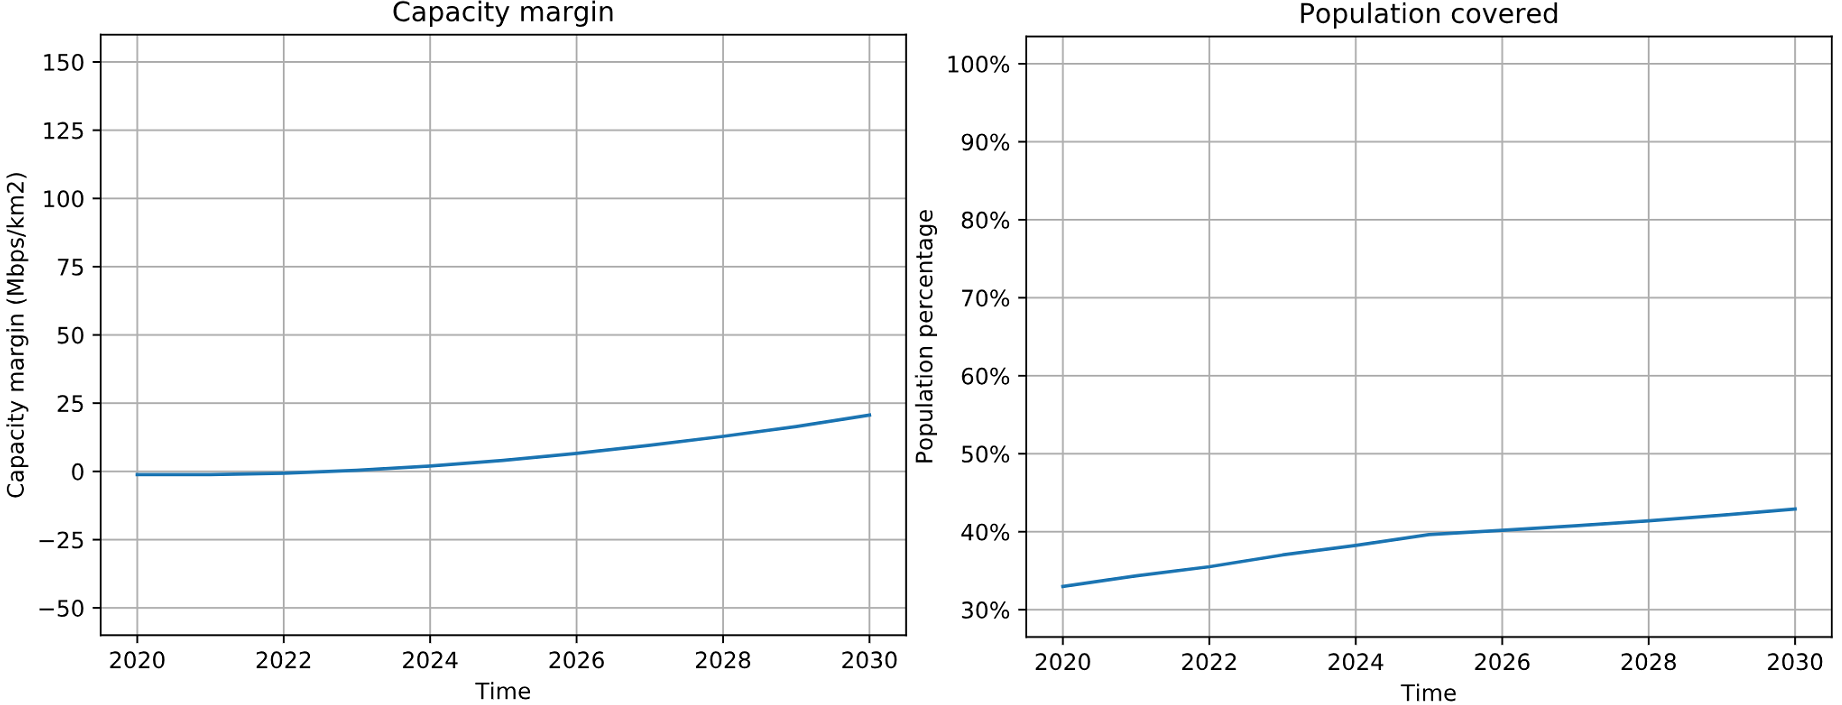
\includegraphics[width=0.90\textwidth]{./media/image69.png}
		\caption{Less profitable areas first - Hybrid strategy. Graph: Capacity margin (left) and population covered (right). Source: Author}
	\end{Center}
\end{figure}


%%%%%%%%%%%%%%%%%%%% Figure/Image No: 15 Ends here %%%%%%%%%%%%%%%%%%%%

Capacity margin grows less than in the previous coverage obligation set. This could be because the telecom operator is investing in the most interesting places, but the reason is that resources are so wasted that capacity margin does not grow either. Population covered has similar values as in the previous obligation. \par



%%%%%%%%%%%%%%%%%%%% Figure/Image No: 16 starts here %%%%%%%%%%%%%%%%%%%%

\begin{figure}[H]
	\begin{Center}
		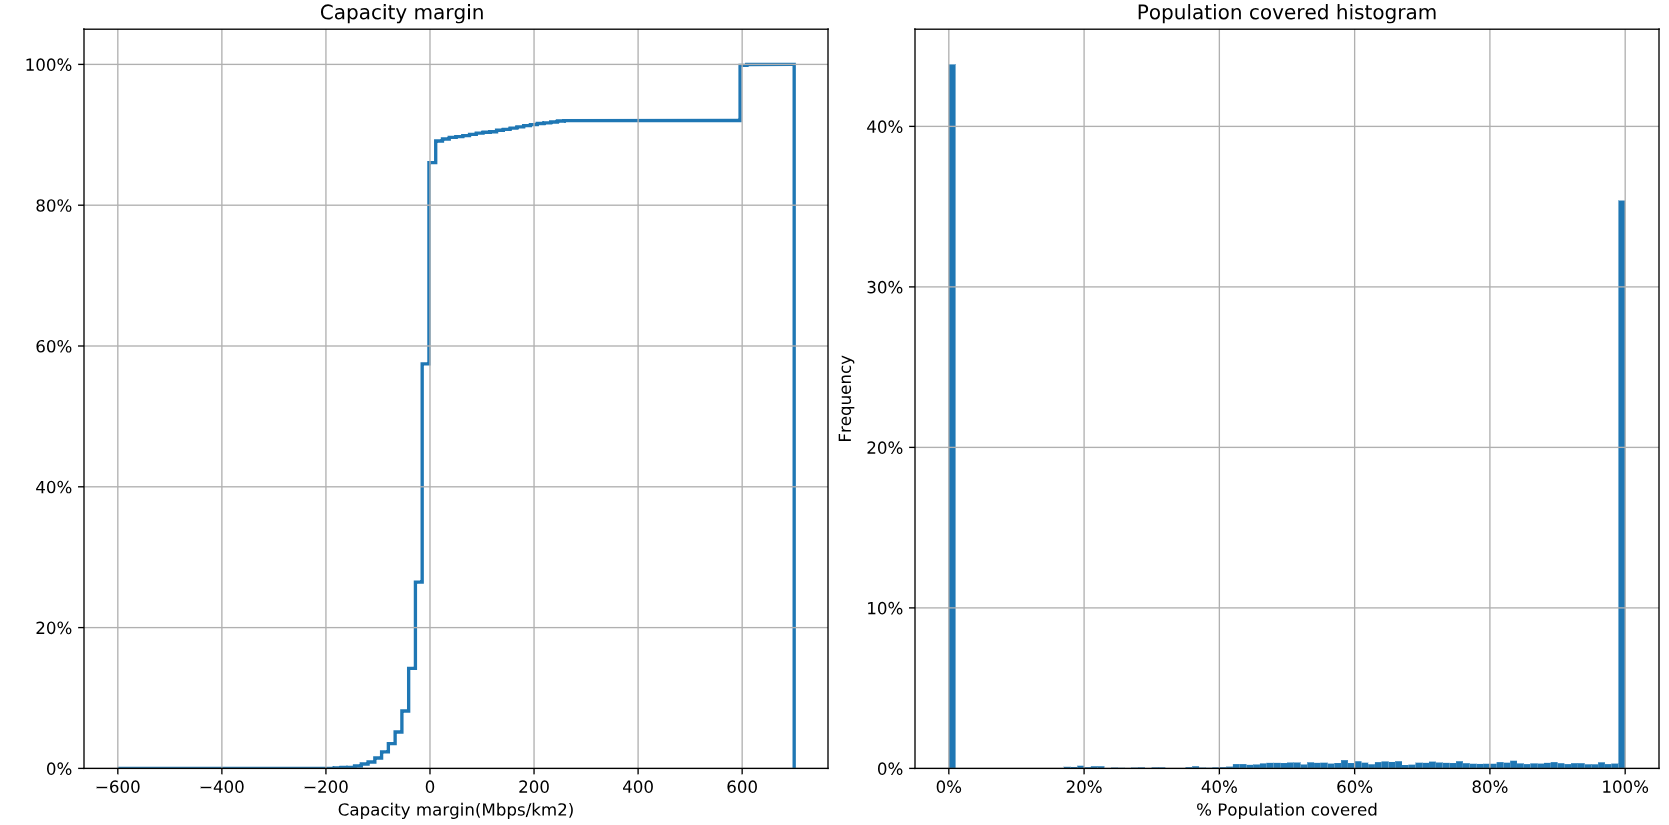
\includegraphics[width=0.90\textwidth]{./media/image70.png}
		\caption{Less profitable areas first - Hybrid strategy. Graph: Capacity margin CDF (left) and population covered histogram (right). Source: Author}
	\end{Center}
\end{figure}


%%%%%%%%%%%%%%%%%%%% Figure/Image No: 16 Ends here %%%%%%%%%%%%%%%%%%%%


As it can be seen, the situation is very similar to the previous coverage obligation set. Capacity margin per PCD is mainly about the 0Mbps/km\textsuperscript{2}, although there is a group of 10$\%$  of the PCDs that have too high capacity margin, about 600Mbps/km\textsuperscript{2} and this waste of resources is what penalizes this strategy. Moreover, we can see in the graph on the right that more than 40$\%$  of the PCDs received no investment and that only 35$\%$  of the PCDs have all of its population with the 2Mbps that the coverage obligation demands.\par

The following coloured map shows the money that has been spent in each LAD during all the execution time. It represents the problem of the unbalanced investment clearly: Most of the investment effort was made in PCDs that are not the most important nor the most densely populated.\par


%%%%%%%%%%%%%%%%%%%% Figure/Image No: 17 starts here %%%%%%%%%%%%%%%%%%%%

\begin{figure}[H]
	\begin{Center}
		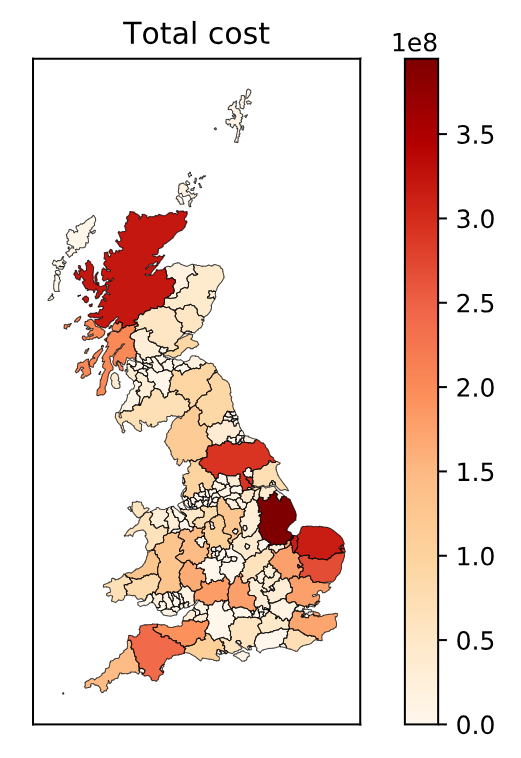
\includegraphics[width=0.55\textwidth]{./media/image71.png}
		\caption{Less profitable areas first - Hybrid strategy. Map: Total cost. Source: Author}
	\end{Center}
\end{figure}


%%%%%%%%%%%%%%%%%%%% Figure/Image No: 17 Ends here %%%%%%%%%%%%%%%%%%%%


This leads us to the graph that compares the population covered by the cost that takes to reach this specific percentage of population covered. As it can be seen, starting with 35$\%$  of the population already fulfilling the coverage obligations, this strategy just increments the coverage by 10$\%$  while it is investing all the resources available.\par



%%%%%%%%%%%%%%%%%%%% Figure/Image No: 18 starts here %%%%%%%%%%%%%%%%%%%%

\begin{figure}[H]
	\begin{Center}
		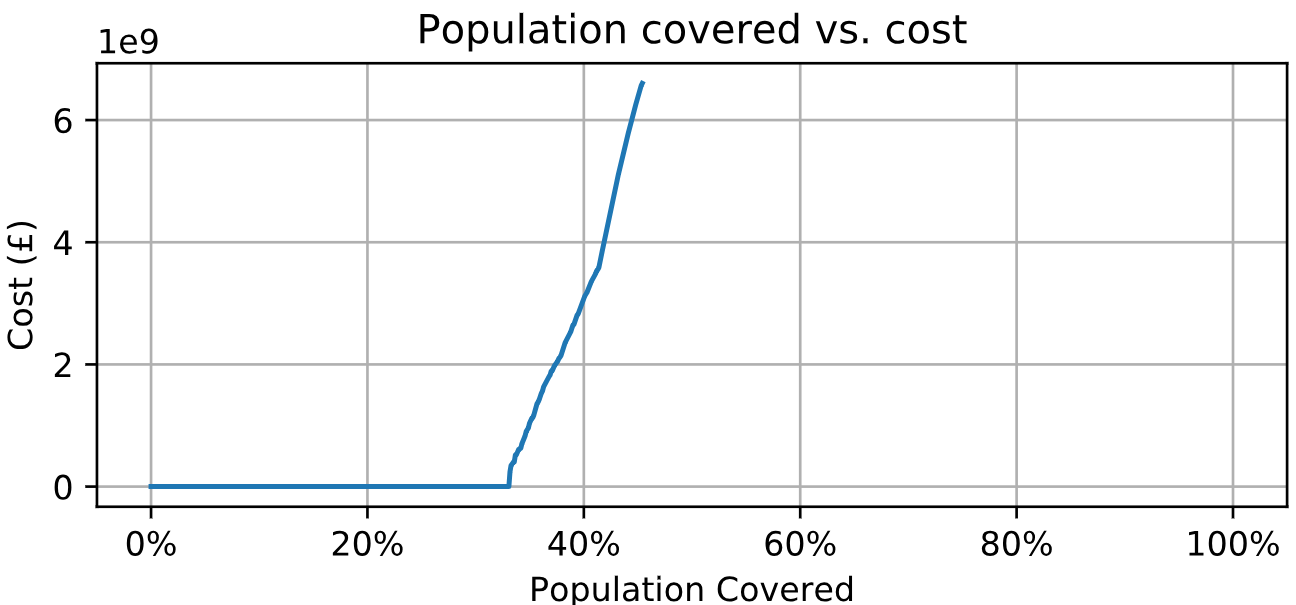
\includegraphics[width=0.73\textwidth]{./media/image72.png}
		\caption{Less profitable areas first - Hybrid strategy. Graph: Population covered vs. cost. Source: Author}
	\end{Center}
\end{figure}


%%%%%%%%%%%%%%%%%%%% Figure/Image No: 18 Ends here %%%%%%%%%%%%%%%%%%%%


In order to have a full picture of this case, the following coloured maps represent the evolution of the coverage obligations over the years and how the investment effort was focused on the bigger LADs, which have normally less population density.\par



%%%%%%%%%%%%%%%%%%%% Figure/Image No: 19 starts here %%%%%%%%%%%%%%%%%%%%

\begin{figure}[H]
	\begin{Center}
		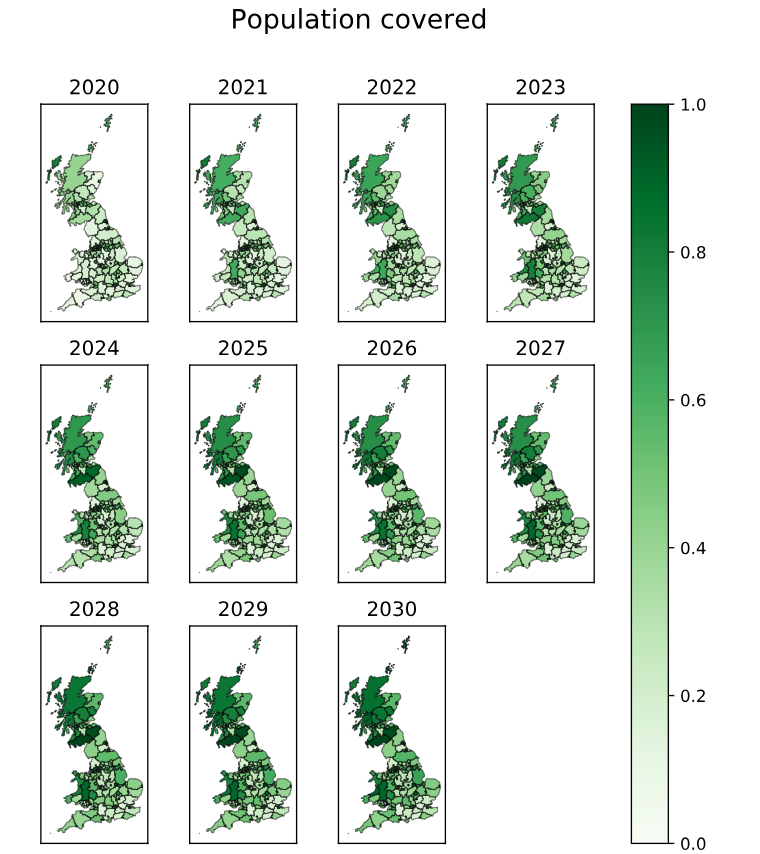
\includegraphics[width=0.75\textwidth]{./media/image73.png}
		\caption{Less profitable areas first - Hybrid strategy. Map: Population covered. Source: Author}
	\end{Center}
\end{figure}


%%%%%%%%%%%%%%%%%%%% Figure/Image No: 19 Ends here %%%%%%%%%%%%%%%%%%%%


As a summary, this coverage obligation set has the same investment effort than �\textit{Priority areas first�} and the increment of the percentage of population covered is similar, but the capacity margin does not increase as much as it does in the other set. Hence, this combination is even less interesting for the telecom operator and the policymakers than the previous one.\par

\paragraph*{No budget limitation}
%\addcontentsline{toc}{paragraph}{No budget limitation}
As it happens with the previous coverage obligation set, using this capacity expansion strategy and disabling the budget limit would allow the telecom operator to invest until it reaches the 100$\%$  of the population covered. The reason why this strategy does not reach the 100$\%$  with the budget limit is that its investments are not efficient and, therefore, the normal budget is not enough. The following graph represents the total investment needed to reach the 100$\%$  of the population covered:\par



%%%%%%%%%%%%%%%%%%%% Figure/Image No: 20 starts here %%%%%%%%%%%%%%%%%%%%

\begin{figure}[H]
	\begin{Center}
		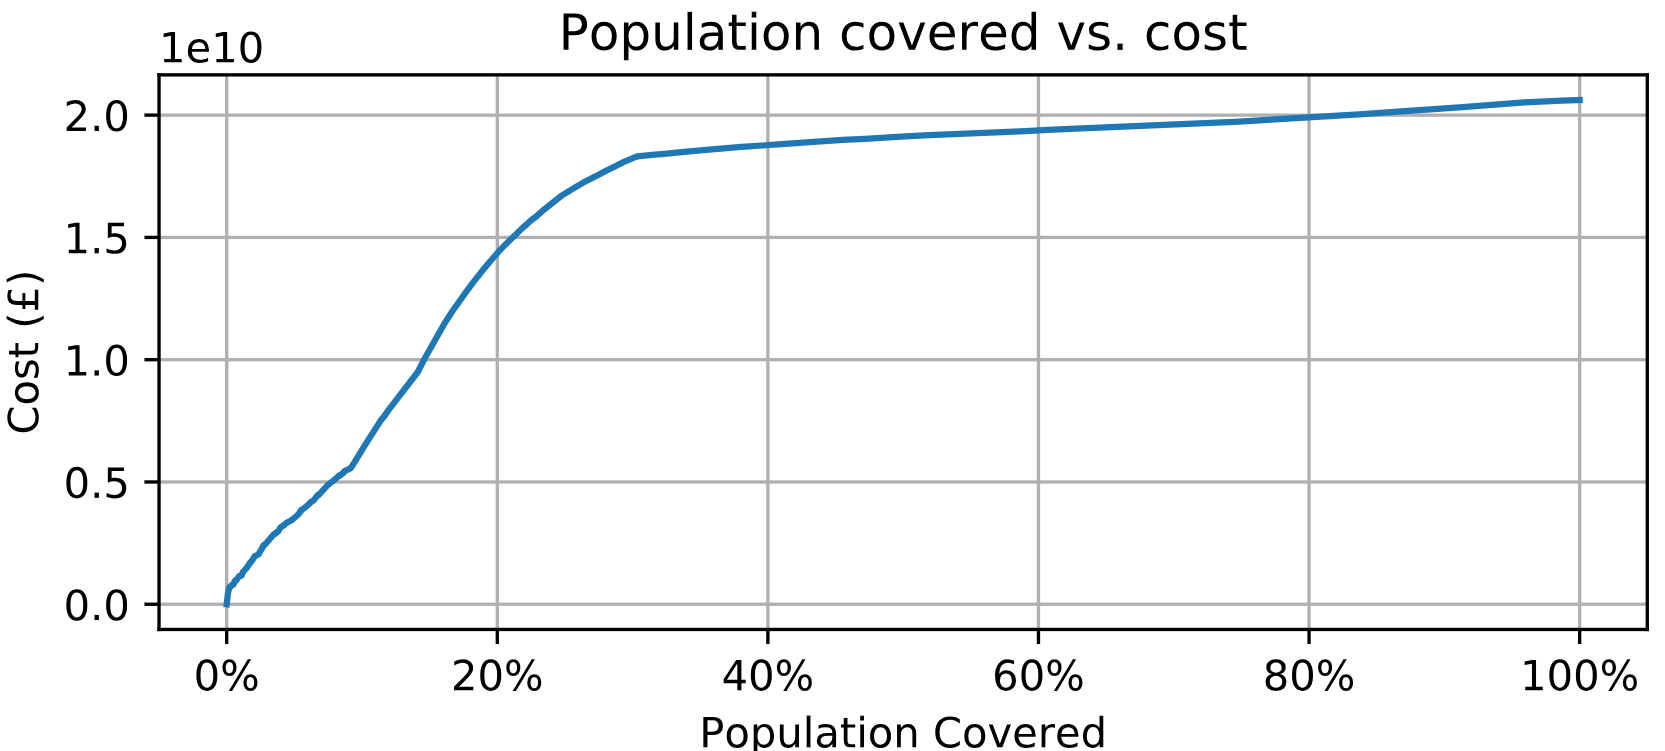
\includegraphics[width=0.75\textwidth]{./media/image74.png}
		\caption{Less profitable areas first - Hybrid strategy. Graph: Population covered vs. cost with budget limit. Source: Author}
	\end{Center}
\end{figure}


%%%%%%%%%%%%%%%%%%%% Figure/Image No: 20 Ends here %%%%%%%%%%%%%%%%%%%%


As it can be seen, the operator would need approximately 3 times the budget estimated for the period. It is also interesting to point out that the curve is smooth, without drastic changes in the direction of the curve, since all the PCDs are ordered according to the population density.\par

\subsubsection*{�700 MHz densification�}
%\addcontentsline{toc}{subsubsection}{�700 MHz densification�}
In this section, we are going to evaluate the most interesting outputs of the \textit{�700 MHz densification� }strategy combined with the\textit{ �Less profitable first� }coverage obligation set. The main outputs are similar to the ones that we had when we combined this strategy with the �\textit{Priority areas first�} obligation since they order PCDs in the same way. For example, aggregation of the capacity margin, the investment and the population covered are similar:\par



%%%%%%%%%%%%%%%%%%%% Figure/Image No: 21 starts here %%%%%%%%%%%%%%%%%%%%

\begin{figure}[H]
	\begin{Center}
		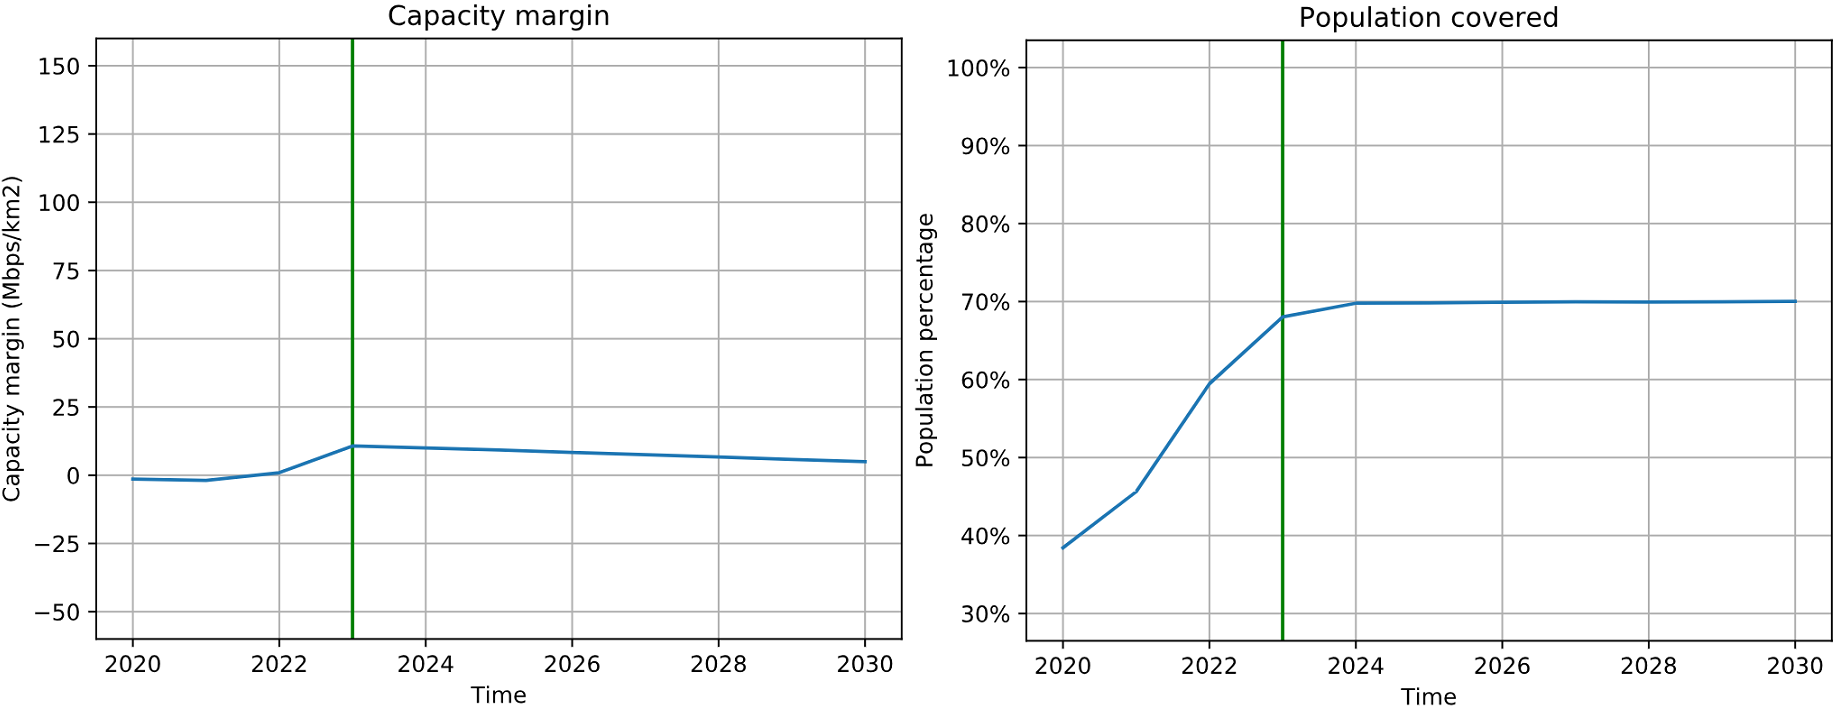
\includegraphics[width=0.95\textwidth]{./media/image75.png}
		\caption{Less profitable areas first - 700 MHz densification. Graph: Capacity margin (left) and population covered (right). Source: Author}
	\end{Center}
\end{figure}


%%%%%%%%%%%%%%%%%%%% Figure/Image No: 21 Ends here %%%%%%%%%%%%%%%%%%%%


It is important to highlight that capacity margin growths during the years that the telecom operator has to invest to meet the coverage obligation and, then, this value goes down again. It is not beneficial for the telecom operator to have a high capacity margin if only 70$\%$  of the people have enough end-user speed to fulfil the coverage obligations.\par

The rest of the graphs are similar to the ones presented in the �\textit{Priority areas first�} coverage obligation, so it makes no sense to repeat them. The following coloured maps represent the evolution of the coverage obligations over the years:\par



%%%%%%%%%%%%%%%%%%%% Figure/Image No: 22 starts here %%%%%%%%%%%%%%%%%%%%

\begin{figure}[H]
	\begin{Center}
		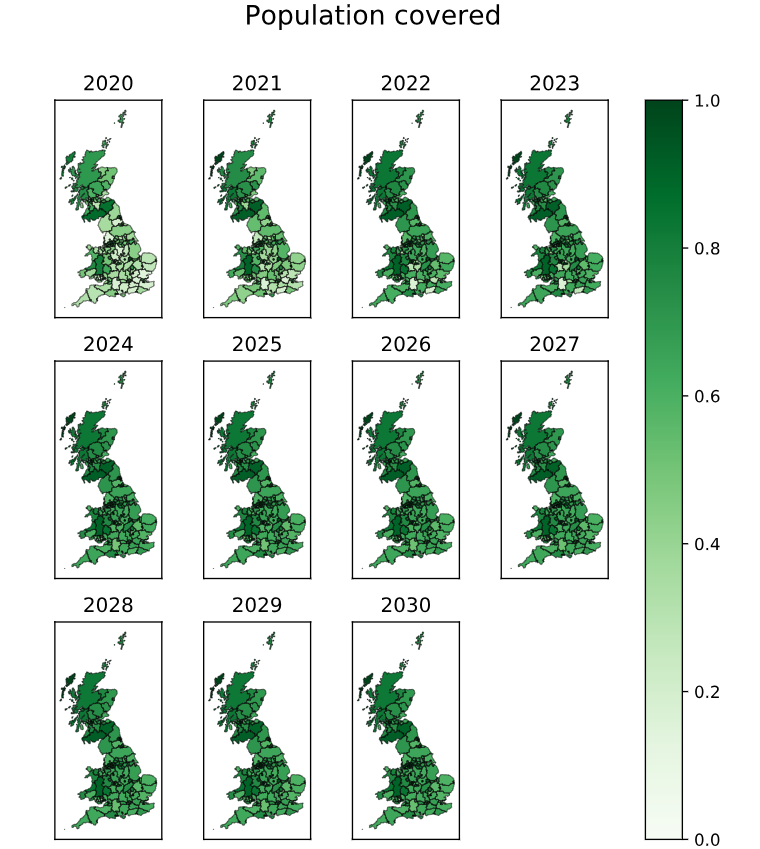
\includegraphics[width=0.95\textwidth]{./media/image76.png}
		\caption{Less profitable areas first - 700 MHz densification. Map: Population covered. Source: Author}
	\end{Center}
\end{figure}


%%%%%%%%%%%%%%%%%%%% Figure/Image No: 22 Ends here %%%%%%%%%%%%%%%%%%%%


Despite the population covered in 2030 is the same, the evolution and the prioritization of LADs to invest first changes between these two coverage obligation sets, since the order in which the algorithm invests is different. As this algorithm starts with the very less profitable PCD, it focuses on the LADs of Scotland and Wales, investing in most regions of England later. However, the overall result is similar.\par

The last output that we are going to analyse is the relation between a certain percentage of population covered and the cost that it takes to obtain it. The following graph represents this relation:\par



%%%%%%%%%%%%%%%%%%%% Figure/Image No: 23 starts here %%%%%%%%%%%%%%%%%%%%

\begin{figure}[H]
	\begin{Center}
		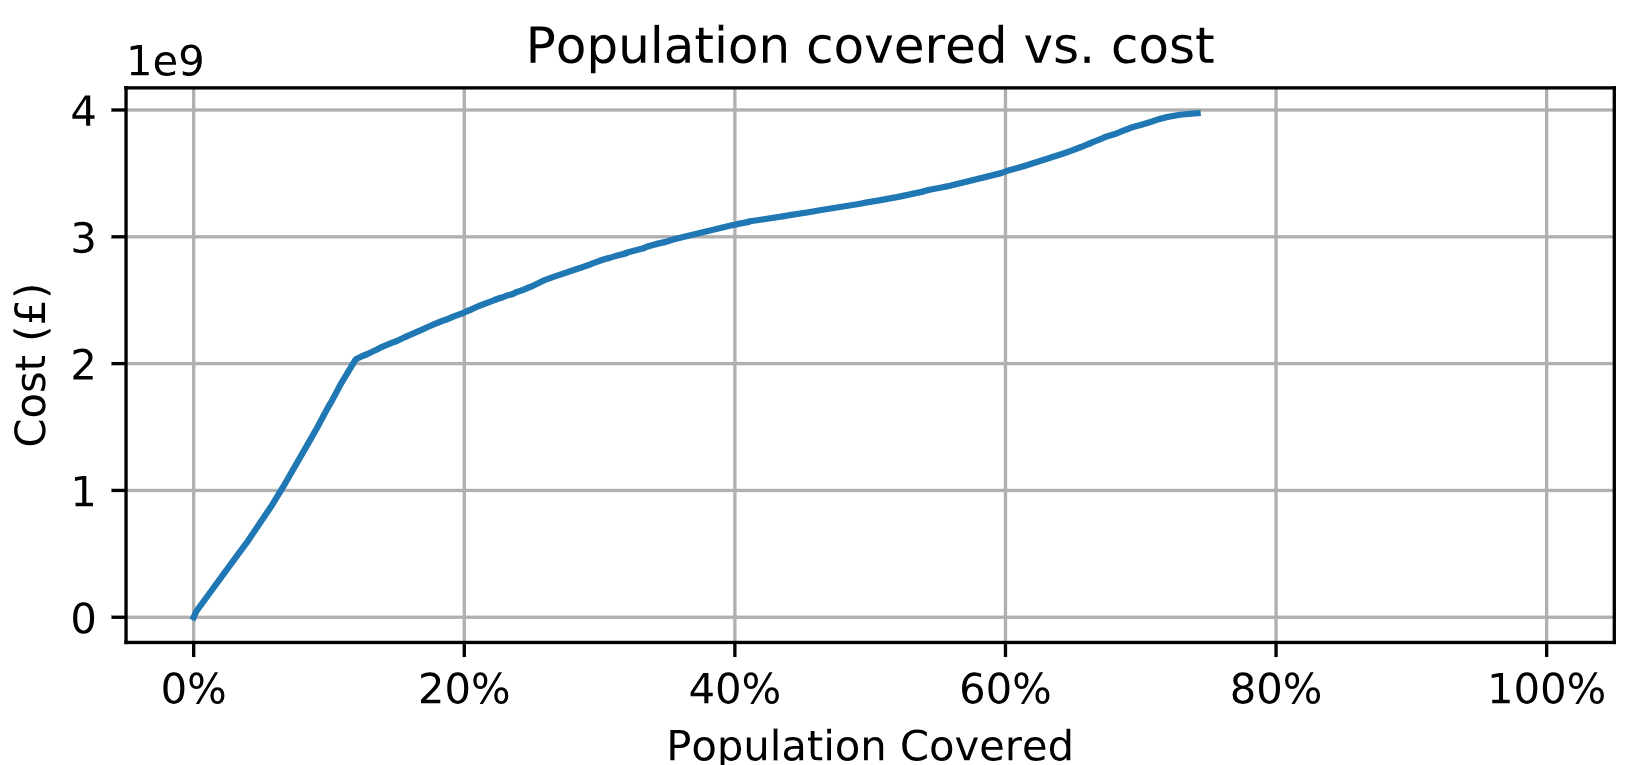
\includegraphics[width=0.75\textwidth]{./media/image77.png}
		\caption{Less profitable areas first - 700 MHz densification. Graph: Population covered vs. cost. Source: Author}
	\end{Center}
\end{figure}


%%%%%%%%%%%%%%%%%%%% Figure/Image No: 23 Ends here %%%%%%%%%%%%%%%%%%%%


The results are similar to the previous ones, the curve is smooth, and it only reaches 70$\%$  of the population.\par

\paragraph*{No budget limitation}
%\addcontentsline{toc}{paragraph}{No budget limitation}
As it happens in the previous coverage obligation, the budget is not the limitation of this coverage obligation. Therefore, despite removing the budget limitation, the results are the same and the population covered vs cost graph has the same values.\par


































\subsection{Only rural areas}
This coverage obligation set defines two groups of PCDs according to their population: (I) PCDS with less than 800 inhabitants (Rural PCDs) and (II) PCDS with more than that (Urban and suburban). Then, operators have to invest first in all the PCDS of the group I before being allowed to build new assets in the group II. As we did before, we are going to see the results of simulations of this coverage obligation set using two different capacity expansion strategies with and without a budget limitation.\par

\subsubsection*{�Hybrid strategy� }
\addcontentsline{toc}{subsubsection}{�Hybrid strategy� }
This coverage obligation set is characterized by its less stringent requirements, which gives the opportunity to the telecom operators to focus earlier in building assets to satisfy the demand instead of using most of its budget in building resources to fulfil the coverage obligations. All the graphs in this section represent a simulation in which the telecom operator creates new assets to meet end-user speed demand after building all the assets of the coverage obligation.\par

The first graphs represent the evolution of the capacity margin and population covered over the years. It is important to remember that, in this simulation, the telecom operator invests all the budget available every year.\par



%%%%%%%%%%%%%%%%%%%% Figure/Image No: 24 starts here %%%%%%%%%%%%%%%%%%%%

\begin{figure}[H]
	\begin{Center}
		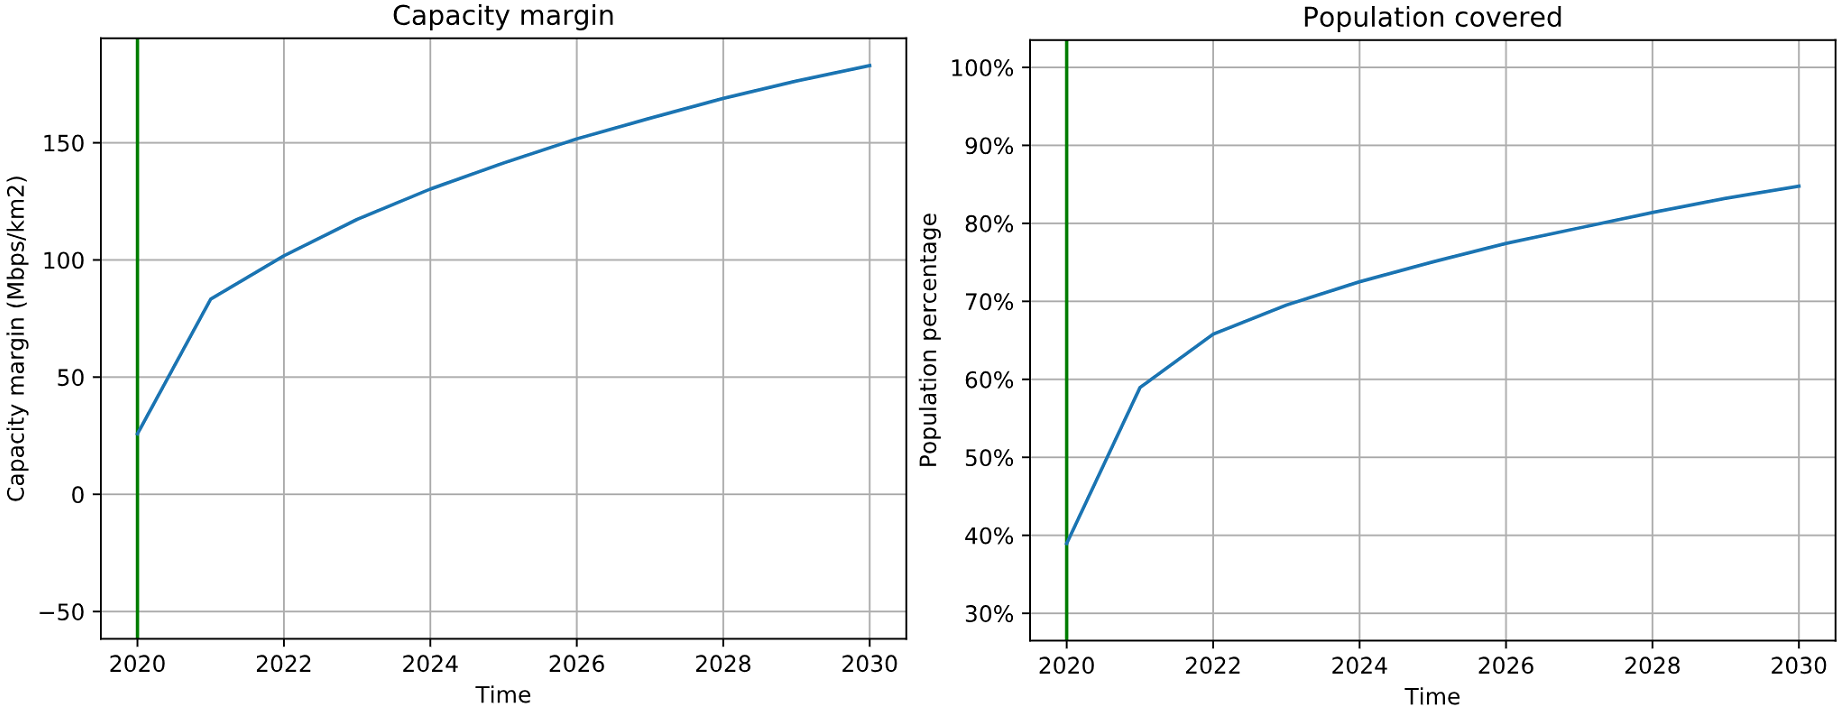
\includegraphics[width=0.95\textwidth]{./media/image78.png}
		\caption{Only rural areas - Hybrid strategy. Graph: Capacity margin (left) and population covered (right). Source: Author}
	\end{Center}
\end{figure}


%%%%%%%%%%%%%%%%%%%% Figure/Image No: 24 Ends here %%%%%%%%%%%%%%%%%%%%

As it can be seen, the evolution of both parameters is much better than in previous coverage obligations. Capacity margin grows rapidly, but this is not bad since the operator invests just where it considers that their users are lack of capacity (The green line represents the change from coverage obligations to demand). The percentage of population covered grows fast, as well, which is even better than the capacity margin. Note that, in this case, as coverage obligations affect so little part of the population of the country, the values of the population covered are calculated as if obligations would affect the whole country. Moreover, the reader should notice that the slope decreases as time goes by since the operator invests first in the more profitable PCDs and then continues with the less profitable ones.\par

Now, we are going to analyse the CDF of the histogram of the capacity margin and the histogram of the population covered, to see how these values are distributed along the territory and check the inequality between territories:\par



%%%%%%%%%%%%%%%%%%%% Figure/Image No: 25 starts here %%%%%%%%%%%%%%%%%%%%

\begin{figure}[H]
	\begin{Center}
		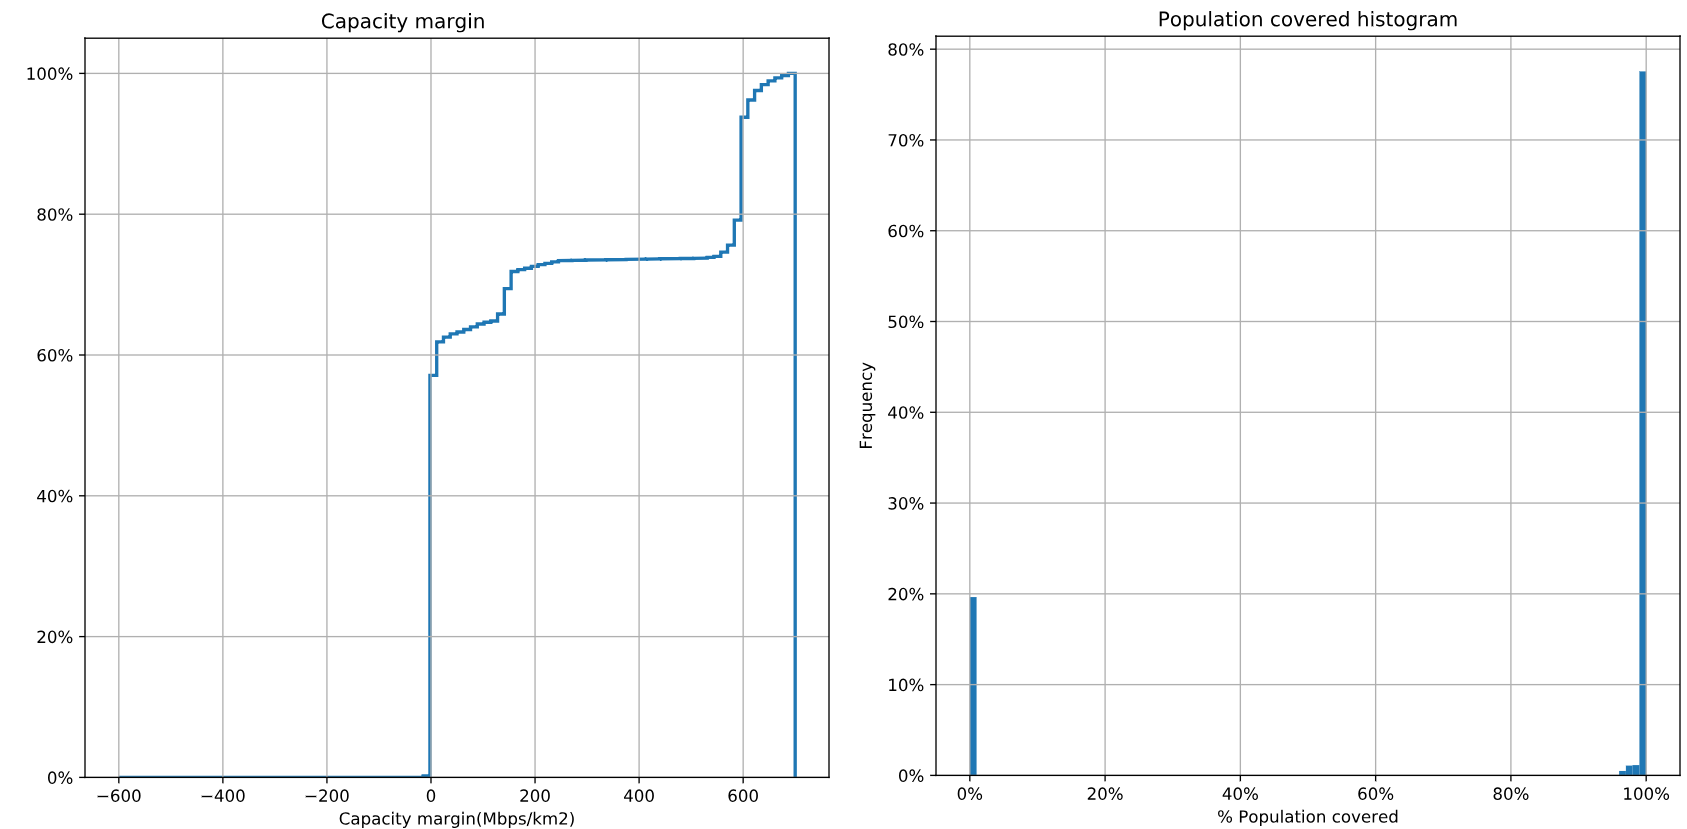
\includegraphics[width=0.95\textwidth]{./media/image79.png}
		\caption{Only rural areas - Hybrid strategy. Graph: Capacity margin CDF (left) and population covered histogram (right). Source: Author}
	\end{Center}
\end{figure}


%%%%%%%%%%%%%%%%%%%% Figure/Image No: 25 Ends here %%%%%%%%%%%%%%%%%%%%


As can be noted from the above charts, after eleven years of investment, the capacity margin of all the regions is at 0 Mbps/km\textsuperscript{2} (50$\%$  of the PCDs) or above (50$\%$  of the PCDs). Even, some of them (25$\%$ ) have a really big capacity margin, which is around 600Mbps/km\textsuperscript{2}. The problem comes with the population covered histogram since results are different from the other executions. In this case, 20$\%$  of the PCDs have no population covered since they received no investment from the telecom operator. On the contrary, almost 80$\%$  of the PCDs have a coverage percentage of 100$\%$ .\par

Now, we are going to see the evolution of the capacity margin and the percentage of population covered. This allows seeing the distribution of these parameters along the national territory:\par



%%%%%%%%%%%%%%%%%%%% Figure/Image No: 26 starts here %%%%%%%%%%%%%%%%%%%%

\begin{figure}[H]
	\begin{Center}
		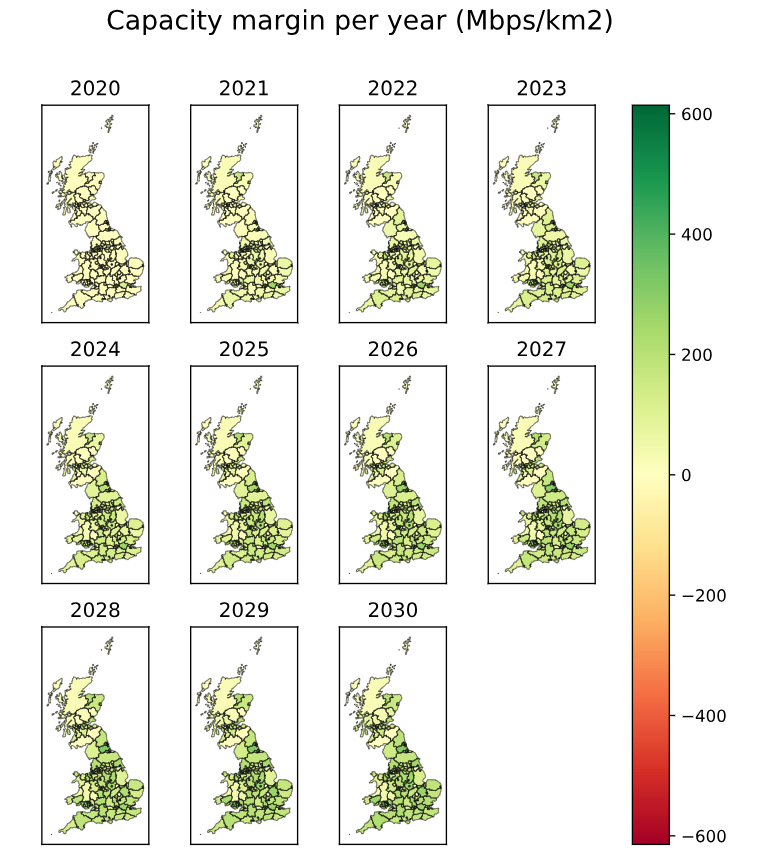
\includegraphics[width=0.95\textwidth]{./media/image80.png}
		\caption{Only rural areas - Hybrid strategy. Map: Capacity margin. Source: Author}
	\end{Center}
\end{figure}


%%%%%%%%%%%%%%%%%%%% Figure/Image No: 26 Ends here %%%%%%%%%%%%%%%%%%%%


The evolution of the capacity margin is very good. Capacity margin reaches 600Mbps/km\textsuperscript{2} in some LADs, which is a lot and no LAD has the capacity margin below 0. It is important to notice that there are more improvements in England instead of been homogeneous in all the countries. The following coloured map represents the evolution of the coverage obligation:\par



%%%%%%%%%%%%%%%%%%%% Figure/Image No: 27 starts here %%%%%%%%%%%%%%%%%%%%

\begin{figure}[H]
	\begin{Center}
		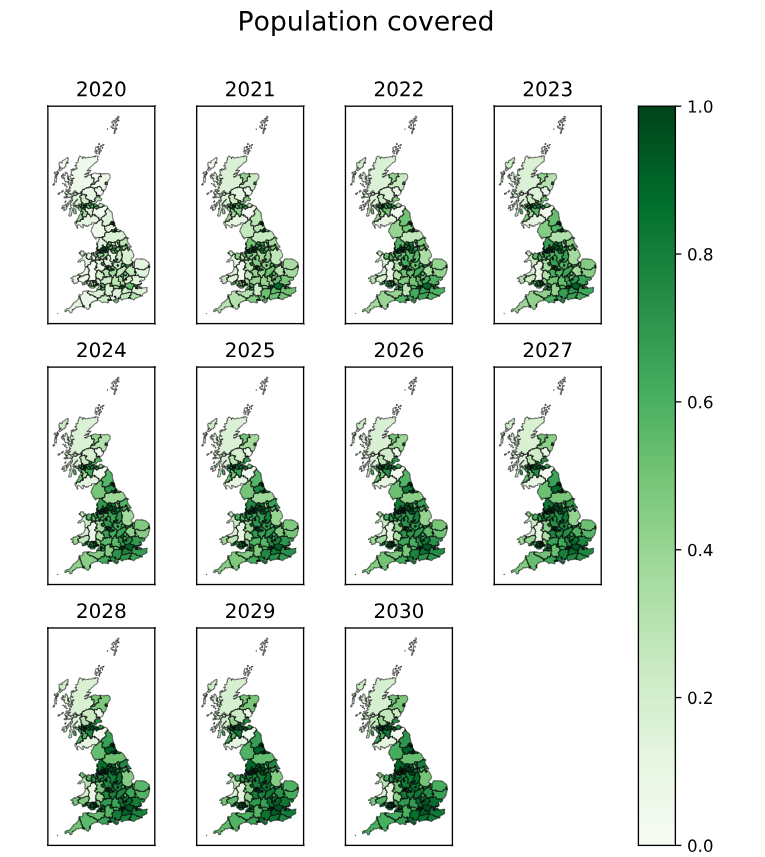
\includegraphics[width=0.95\textwidth]{./media/image81.png}
		\caption{Only rural areas - Hybrid strategy. Map: Population covered. Source: Author}
	\end{Center}
\end{figure}


%%%%%%%%%%%%%%%%%%%% Figure/Image No: 27 Ends here %%%%%%%%%%%%%%%%%%%%


This time, something similar to the capacity margin happens with the percentage of population covered in each LAD: Values are better than using other coverage obligation sets, but they are focused on England, while values in Scotland and Wales are smaller.\par

Finally, we are going to analyse the population covered vs. cost graph. As it can be seen, coverage obligations only affect a little part of the whole population of the country. After an almost-vertical slope of 1$\%$  or 2$\%$  of the population, the telecom operator has fulfilled the coverage obligations and starts investing in prioritizing the profitability.\par



%%%%%%%%%%%%%%%%%%%% Figure/Image No: 28 starts here %%%%%%%%%%%%%%%%%%%%

\begin{figure}[H]
	\begin{Center}
		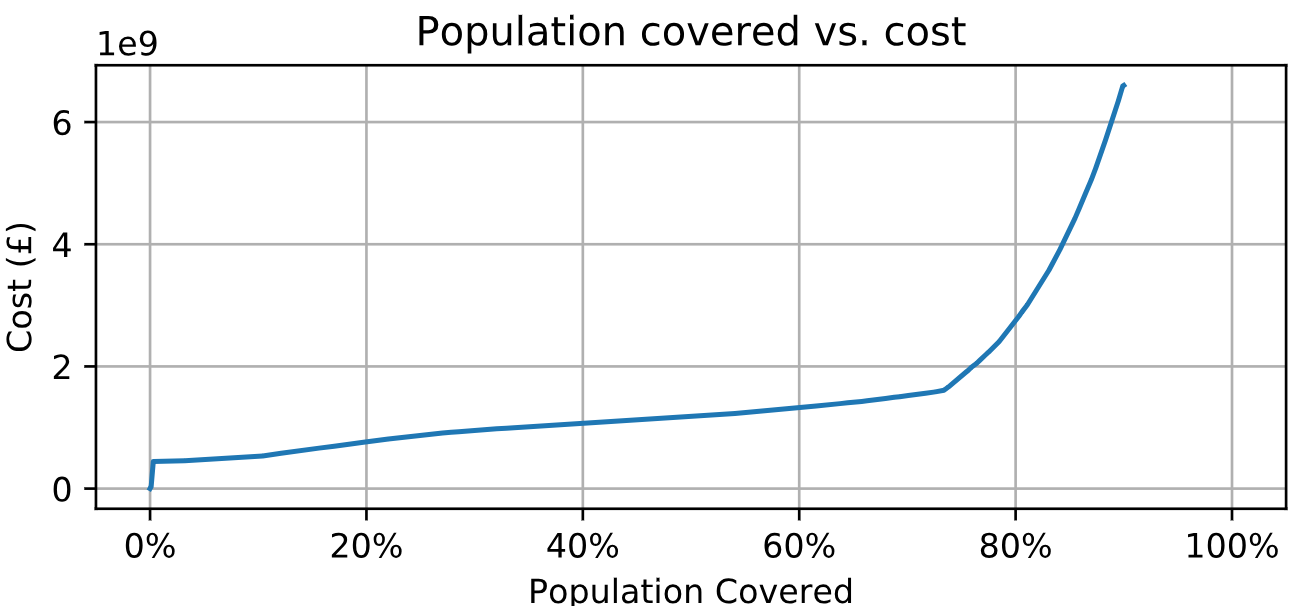
\includegraphics[width=0.75\textwidth]{./media/image82.png}
		\caption{Only rural areas - Hybrid strategy. Graph: Population covered vs. cost. Source: Author}
	\end{Center}
\end{figure}


%%%%%%%%%%%%%%%%%%%% Figure/Image No: 28 Ends here %%%%%%%%%%%%%%%%%%%%


In general, results are not bad, but the reality is that they are similar to the ones obtained when there are no coverage obligation sets and the policymaker allows telecom operators to decide which are the most suitable PCDs to invest. \par

\paragraph*{No budget limitation}
%\addcontentsline{toc}{paragraph}{No budget limitation}
Now we are going to see how removing the budget limitation affects the population covered. The following graph represents the same values as above, but in a simulation where there is no budget limitation.\par



%%%%%%%%%%%%%%%%%%%% Figure/Image No: 29 starts here %%%%%%%%%%%%%%%%%%%%

\begin{figure}[H]
	\begin{Center}
		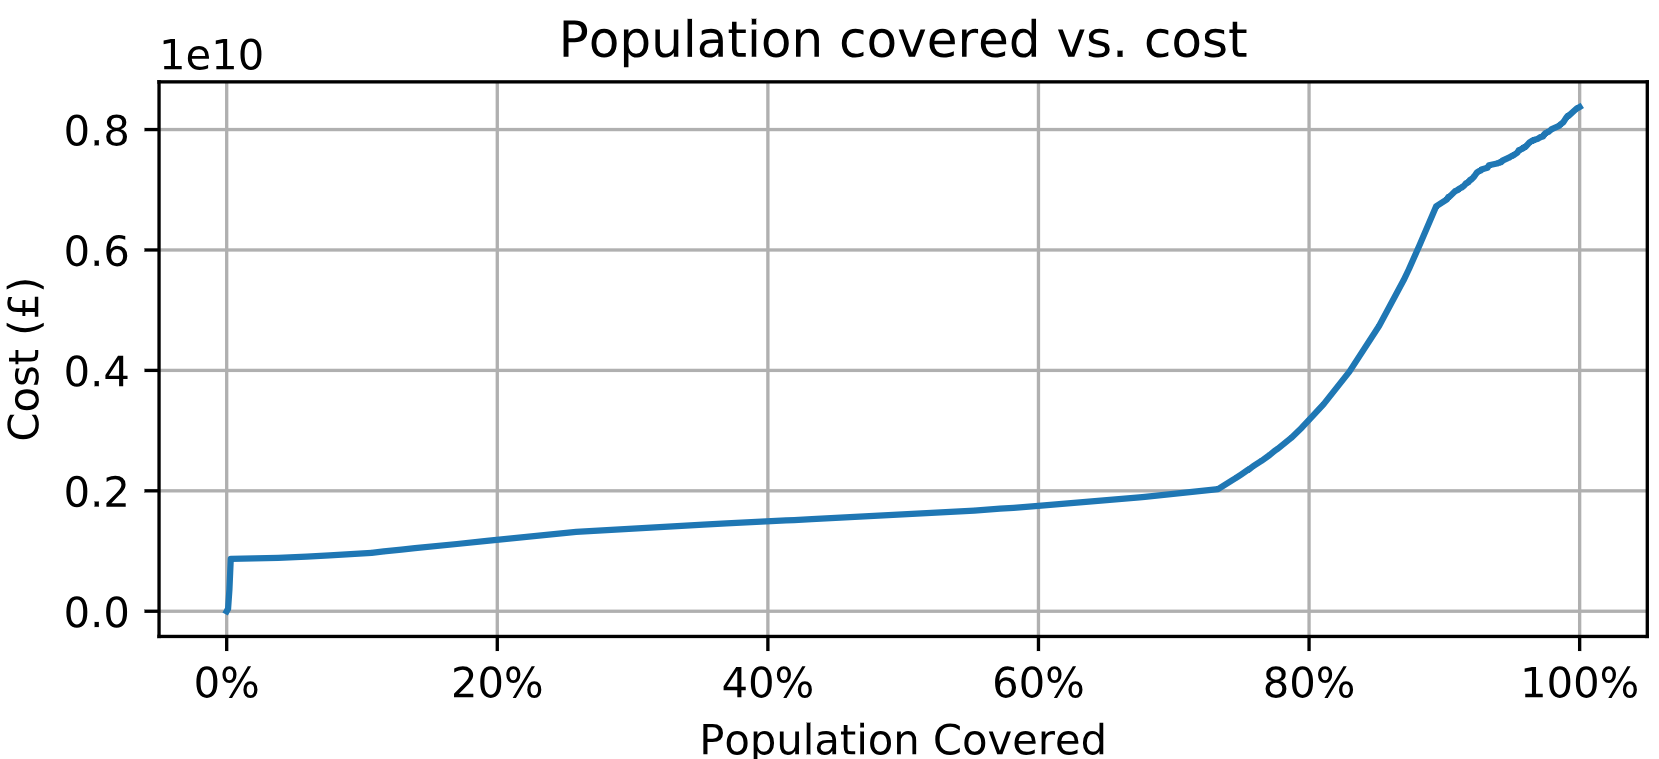
\includegraphics[width=0.75\textwidth]{./media/image83.png}
		\caption{Only rural areas - Hybrid strategy. Graph: Population covered vs. cost without budget limitation. Source: Author}
	\end{Center}
\end{figure}


%%%%%%%%%%%%%%%%%%%% Figure/Image No: 29 Ends here %%%%%%%%%%%%%%%%%%%%


As it can be seen, the limitations where only due to the budget and removing this limitation, the remaining 12$\%$  of the population can be covered using almost 30$\%$  more budget.\par

\subsubsection*{�700 MHz densification�}
%\addcontentsline{toc}{subsubsection}{�700 MHz densification�}
In this section, we are going to evaluate how the \textit{�700 MHz densification�} capacity expansion strategy behaves with the �\textit{Only rural areas�} coverage obligation. As we have done in the previous analysis, we are going to check if the telecom operator builds assets at its maximum capacity during the whole execution:\par



%%%%%%%%%%%%%%%%%%%% Figure/Image No: 30 starts here %%%%%%%%%%%%%%%%%%%%

\begin{figure}[H]
	\begin{Center}
		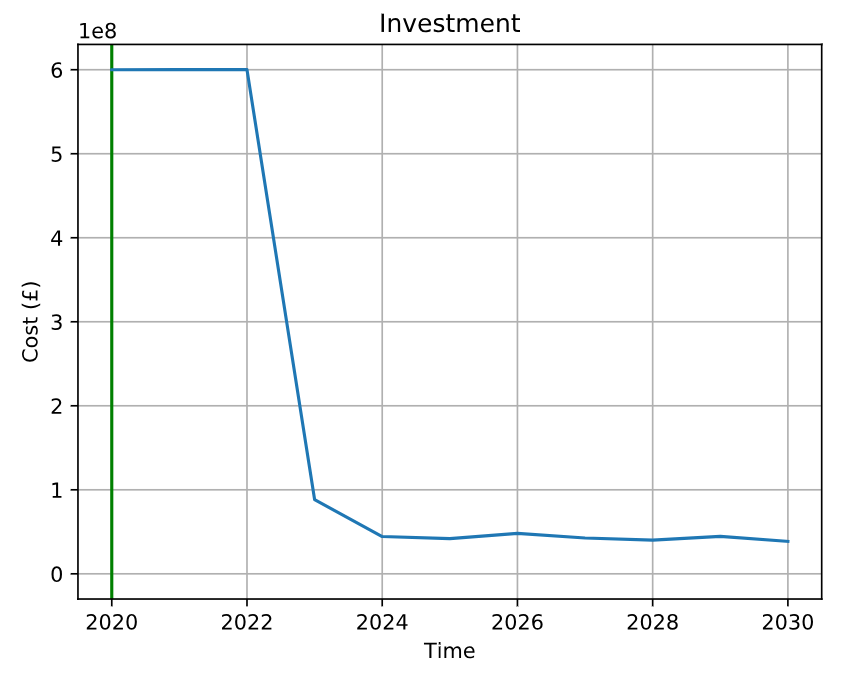
\includegraphics[width=0.75\textwidth]{./media/image84.png}
		\caption{Only rural areas - 700 MHz densification. Graph: Investment. Source: Author}
	\end{Center}
\end{figure}


%%%%%%%%%%%%%%%%%%%% Figure/Image No: 30 Ends here %%%%%%%%%%%%%%%%%%%%


As we can see in the graph, the telecom operator does not maximize its investment capabilities. This could be due to technical issues or because it has fulfilled the coverage obligations before the end of the execution. In the following graphs we can see the evolution of the capacity margin and the population covered:\par



%%%%%%%%%%%%%%%%%%%% Figure/Image No: 31 starts here %%%%%%%%%%%%%%%%%%%%

\begin{figure}[H]
	\begin{Center}
		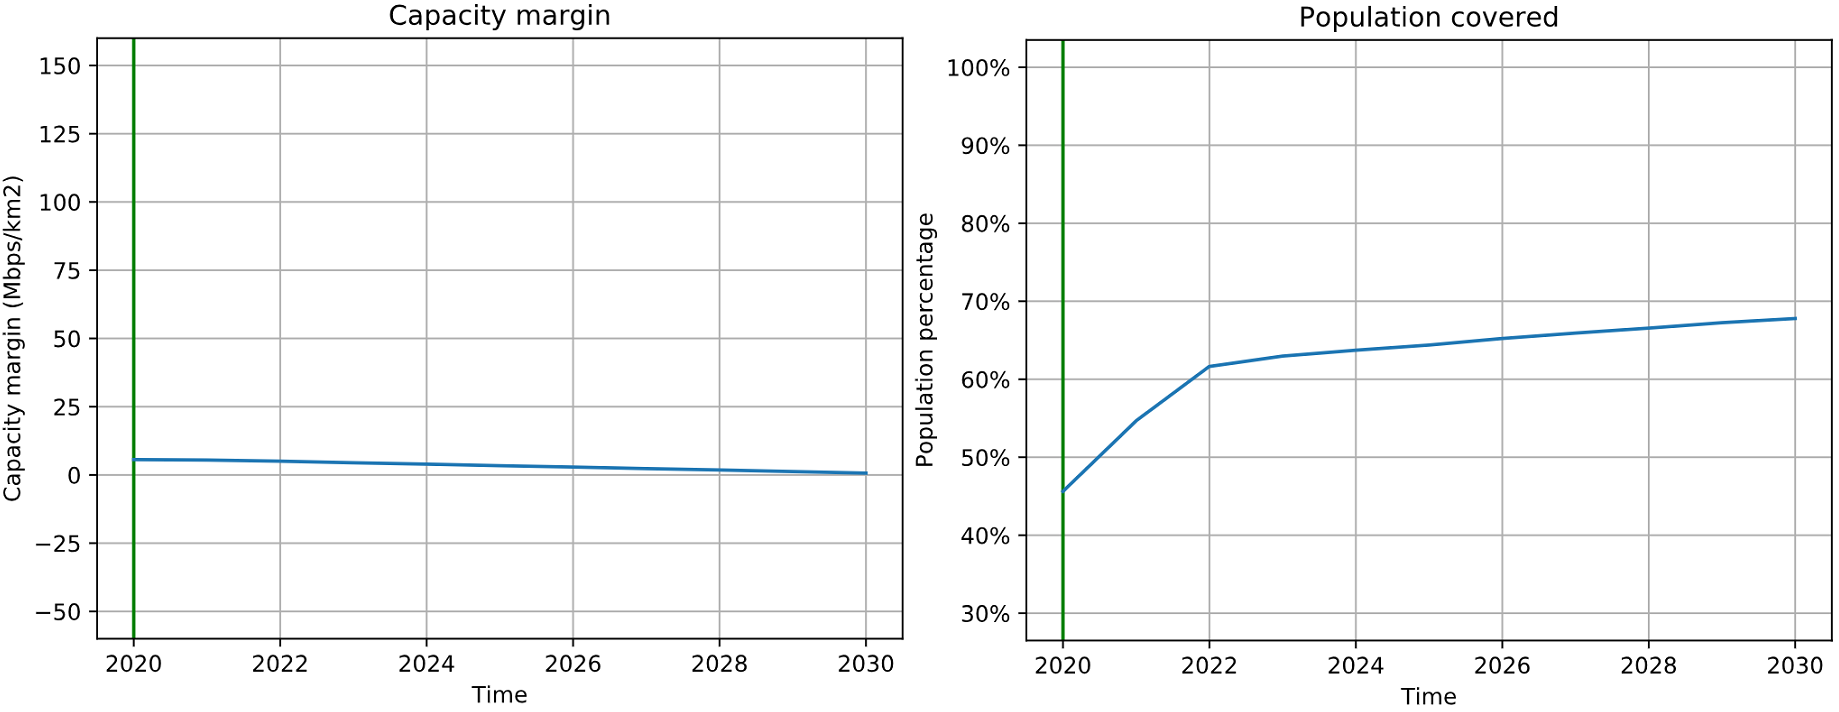
\includegraphics[width=0.95\textwidth]{./media/image85.png}
		\caption{Only rural areas - 700 MHz densification. Graph: Capacity margin and population covered. Source: Author}
	\end{Center}
\end{figure}


%%%%%%%%%%%%%%%%%%%% Figure/Image No: 31 Ends here %%%%%%%%%%%%%%%%%%%%


As it can be seen, the evolution is similar to the previous executions. The capacity margin remains stable during the whole execution since the telecom operator invests only where there is a capacity deficit. On the contrary, the percentage of population covered grows until almost 70$\%$ . As we have seen before, this is the capacity limit of this band.  The histograms of capacity margin and percentage of population covered have a higher detail analysis:\par



%%%%%%%%%%%%%%%%%%%% Figure/Image No: 32 starts here %%%%%%%%%%%%%%%%%%%%

\begin{figure}[H]
	\begin{Center}
		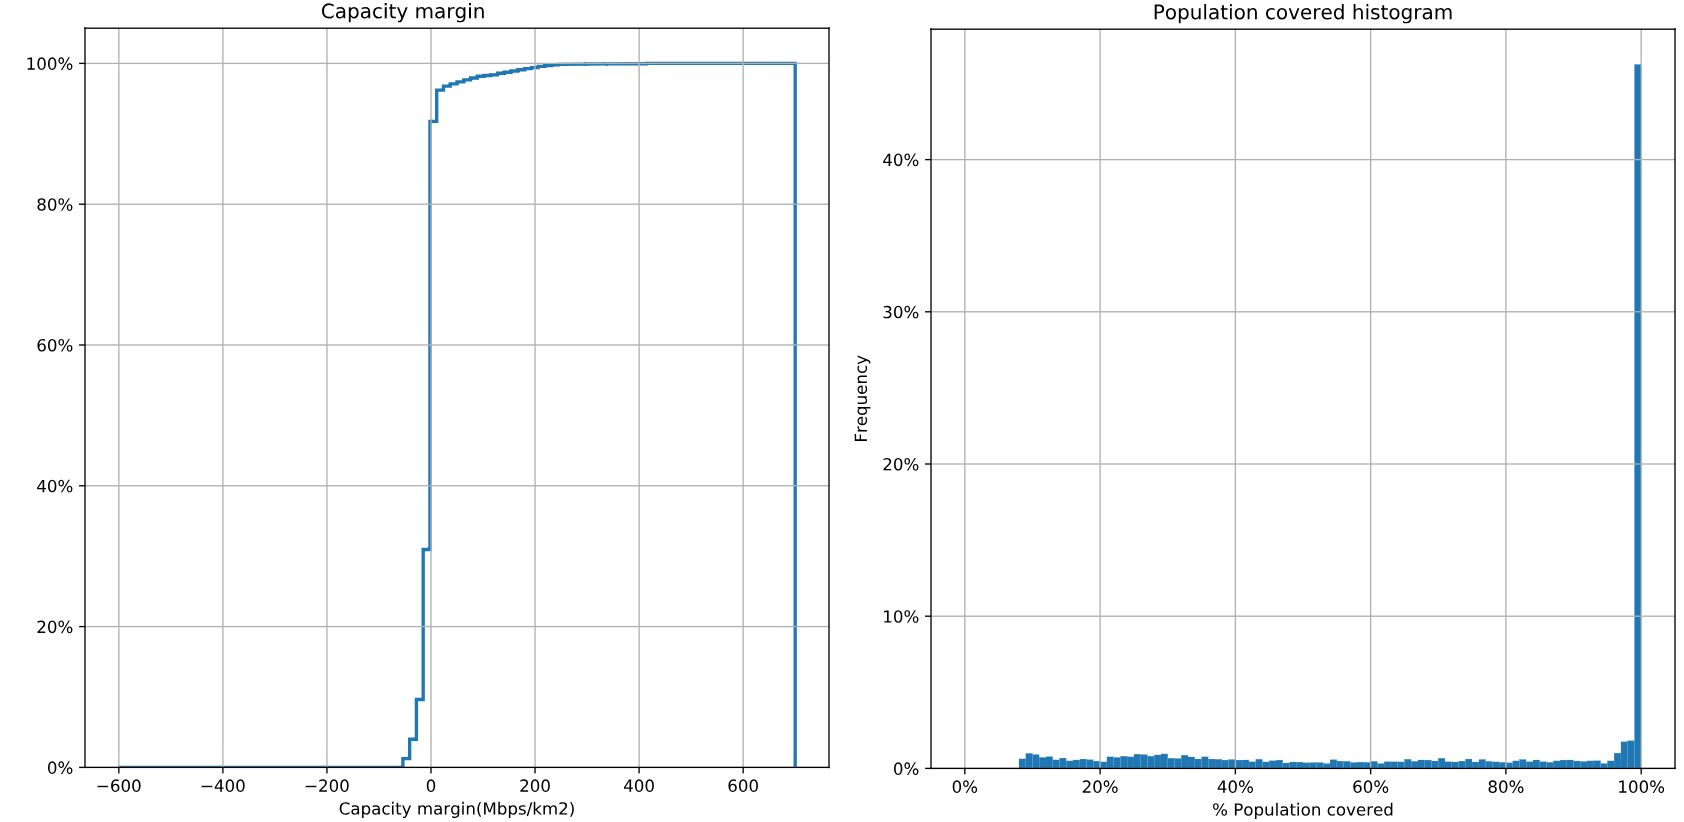
\includegraphics[width=0.95\textwidth]{./media/image86.png}
		\caption{Only rural areas - 700 MHz densification. Histogram: Capacity margin and population covered. Source: Author}
	\end{Center}
\end{figure}


%%%%%%%%%%%%%%%%%%%% Figure/Image No: 32 Ends here %%%%%%%%%%%%%%%%%%%%


As it can be seen, the capacity margin has low dispersion and all the values are around 0 Mbps/km\textsuperscript{2}, which is a good output. It means that all the capacity installed in the network is been harnessed and that capacity is increased on demand. On the contrary, the population covered histogram shows that more than half of the PCDs have some population that does not have enough capacity to fulfil the coverage obligations.\par

The following graph represents the comparison between investment and population covered. The graph shows that the first 2$\%$  of the population is so expensive since they are the most rural PCDs and after that, the telecom operator starts investing in the most profitable PCDs and then continues with the rest of them.\par



%%%%%%%%%%%%%%%%%%%% Figure/Image No: 33 starts here %%%%%%%%%%%%%%%%%%%%

\begin{figure}[H]
	\begin{Center}
		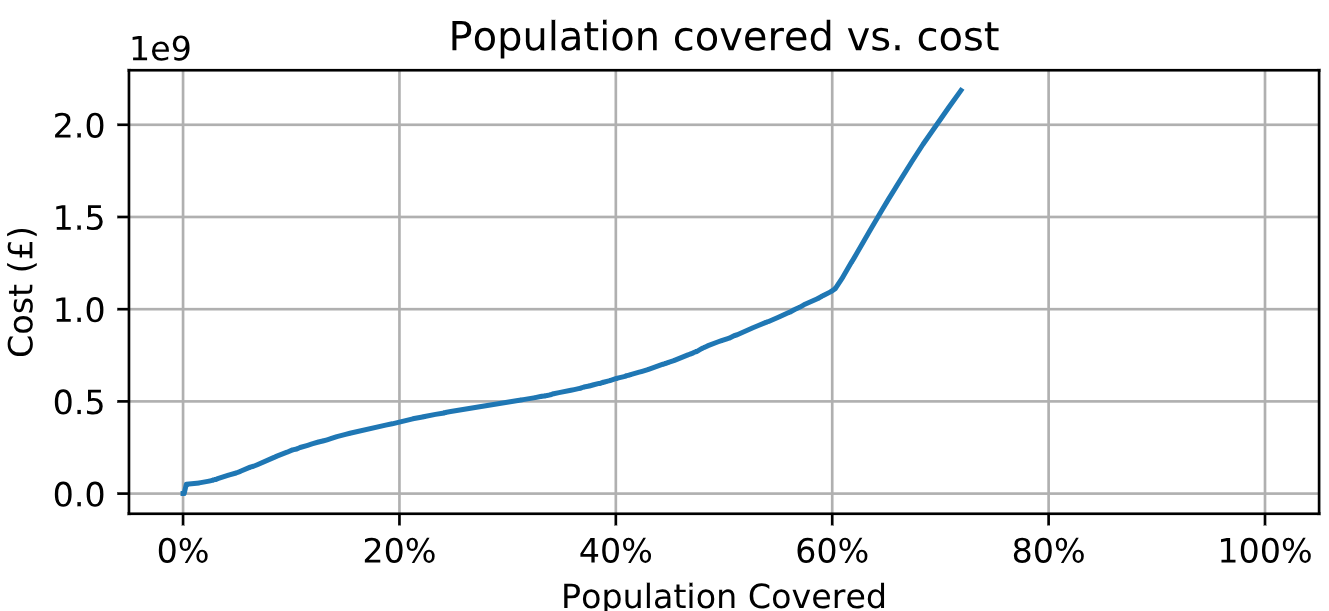
\includegraphics[width=0.75\textwidth]{./media/image87.png}
		\caption{Only rural areas - 700 MHz densification. Graph: Population covered vs. cost. Source: Author}
	\end{Center}
\end{figure}


%%%%%%%%%%%%%%%%%%%% Figure/Image No: 33 Ends here %%%%%%%%%%%%%%%%%%%%


Finally, we are going to check the evolution of the capacity margin and population covered for year and LAD to compare it with the other capacity expansion strategy:\par


%%%%%%%%%%%%%%%%%%%% Figure/Image No: 33 starts here %%%%%%%%%%%%%%%%%%%%

\begin{figure}[H]
	\begin{Center}
		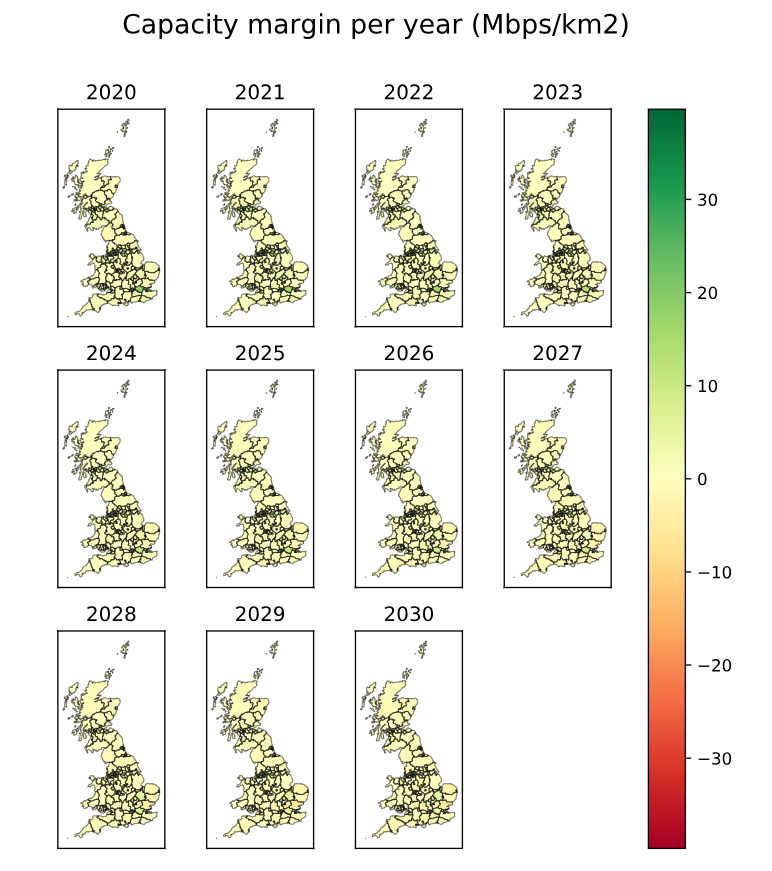
\includegraphics[width=0.95\textwidth]{./media/image88.png}
		\caption{Only rural areas - 700 MHz densification. Map: Capacity margin. Source: Author}
	\end{Center}
\end{figure}


%%%%%%%%%%%%%%%%%%%% Figure/Image No: 33 Ends here %%%%%%%%%%%%%%%%%%%%


As it can be seen, the capacity margin is considerably lower using this strategy instead of the \textit{�Hybrid strategy�} and this is because of the technical limitations of the 700 MHz band. The previous strategy is allowed to combine several bands and, therefore, obtains a higher capacity. The following coloured maps represent the evolution of the population covered:\par


%%%%%%%%%%%%%%%%%%%% Figure/Image No: 33 starts here %%%%%%%%%%%%%%%%%%%%

\begin{figure}[H]
	\begin{Center}
		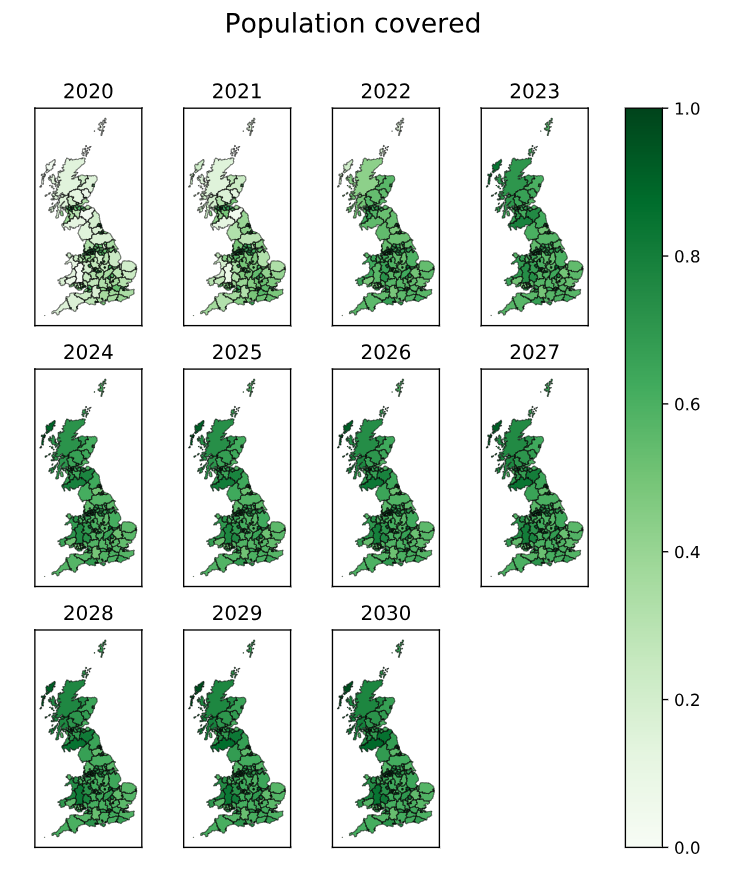
\includegraphics[width=0.95\textwidth]{./media/image89.png}
		\caption{Only rural areas - 700 MHz densification. Map: Population covered. Source: Author}
	\end{Center}
\end{figure}


%%%%%%%%%%%%%%%%%%%% Figure/Image No: 33 Ends here %%%%%%%%%%%%%%%%%%%%


This graph shows a more homogeneous distribution of the population covered since this strategy invests in all the areas (We can know it looking to the investment graph, that shows that has more budget available and not used), but most of the regions do not have 100$\%$  of coverage.\par

As a conclusion, we can observe here that as the issue with this capacity expansion strategy is related to the maximum capacity of the 700 MHz band, enabling the telecom operator to decide in which PCDs it can focus gives no big advantage compared to not enforcing any coverage obligation.\par

\paragraph*{No budget limitation}
%\addcontentsline{toc}{paragraph}{No budget limitation}
The result of the execution when there is no budget limitation is the same as when it is limited. The problem with this capacity expansion strategy is that it only has one band to give all the capacity that the country needs.\par

%%%%%%%%%%%%%%%%%%%% Figure/Image No: 33 starts here %%%%%%%%%%%%%%%%%%%%

\begin{figure}[H]
	\begin{Center}
		\includegraphics[width=0.75\textwidth]{./media/image90.png}
		\caption{Only rural areas - 700 MHz densification. Graph: Population covered vs. cost without budget limitation. Source: Author}
	\end{Center}
\end{figure}


%%%%%%%%%%%%%%%%%%%% Figure/Image No: 33 Ends here %%%%%%%%%%%%%%%%%%%%































\subsection{Nation-balanced}
This is the last coverage obligation set that we are going to study. It orders all the PCDs from more profitable to less and forces the telecom operator to invest until 95$\%$  of the population of each nation has at least the capacity that the coverage obligation demand.\par

\subsubsection*{�Hybrid strategy� }
%\addcontentsline{toc}{subsubsection}{�Hybrid strategy� }
This strategy, as it happens before, does not stop building new assets in all the time of execution. This effort results in the following evolution of the total capacity margin and population covered:\par


%%%%%%%%%%%%%%%%%%%% Figure/Image No: 33 starts here %%%%%%%%%%%%%%%%%%%%

\begin{figure}[H]
	\begin{Center}
		\includegraphics[width=0.95\textwidth]{./media/image91.png}
		\caption{Nation-balanced - Hybrid strategy. Graph: Capacity margin and population covered. Source: Author}
	\end{Center}
\end{figure}


%%%%%%%%%%%%%%%%%%%% Figure/Image No: 33 Ends here %%%%%%%%%%%%%%%%%%%%
As it can be seen, capacity margin grows faster than in all the previous execution and reaches more than 200 Mbps/km\textsuperscript{2} at the end of the execution. The population covered percentage also evolves very well and grows from 32$\%$  of the population covered (Before the year 2020) to approximately 85$\%$  which is more than doubling its original value. However, before stating that this is the best combination, it is important to see the distribution of the capacity along the territory. First, we are going to analyse the capacity margin and population covered histograms:\par


%%%%%%%%%%%%%%%%%%%% Figure/Image No: 33 starts here %%%%%%%%%%%%%%%%%%%%

\begin{figure}[H]
	\begin{Center}
		\includegraphics[width=0.95\textwidth]{./media/image92.png}
		\caption{Nation-balanced - Hybrid strategy. Graph: Capacity margin CDF (left) and population covered histogram (right). Source: Author}
	\end{Center}
\end{figure}


%%%%%%%%%%%%%%%%%%%% Figure/Image No: 33 Ends here %%%%%%%%%%%%%%%%%%%%
The capacity margin histogram represents good results since only 5$\%$  of the population is under 0 Mbps/km\textsuperscript{2}, but also shows that more than 30$\%$  of the PCDs have more than 150 Mbps/km\textsuperscript{2} of capacity overflow, which is a waste of resources and budget. This waste is especially harmful when we consider the histogram of the population covered, too. This histogram shows that more than 20$\%$  of the PCDs have 0$\%$  of the population covered, which means that they received no investment in their region. This is a clear signal of an unbalanced investment across the territory.\par

The next graph shows the cost of increasing the percentage of population covered. As it can be seen, the graph has a very interesting shape for the telecom operators since the cost of the first part is very low and just when there is a significant part of the population covered, the cost of raising the population covered percentage turns prohibitive.\par


%%%%%%%%%%%%%%%%%%%% Figure/Image No: 33 starts here %%%%%%%%%%%%%%%%%%%%

\begin{figure}[H]
	\begin{Center}
		\includegraphics[width=0.75\textwidth]{./media/image93.png}
		\caption{Nation-balanced - Hybrid strategy. Graph: Population covered vs. cost. Source: Author}
	\end{Center}
\end{figure}


%%%%%%%%%%%%%%%%%%%% Figure/Image No: 33 Ends here %%%%%%%%%%%%%%%%%%%%
To see the real impact on the territory, we are going to analyse two groups of coloured maps. The first shows the evolution of the population covered and the second one shows the evolution of the percentage of population covered:\par


%%%%%%%%%%%%%%%%%%%% Figure/Image No: 33 starts here %%%%%%%%%%%%%%%%%%%%

\begin{figure}[H]
	\begin{Center}
		\includegraphics[width=0.95\textwidth]{./media/image94.png}
		\caption{Nation-balanced - Hybrid strategy. Map: Capacity margin. Source: Author}
	\end{Center}
\end{figure}


%%%%%%%%%%%%%%%%%%%% Figure/Image No: 33 Ends here %%%%%%%%%%%%%%%%%%%%
As it can be seen, using this combination of coverage obligation and capacity strategy increases the differences along the country. Those regions that are more densely populated (They are mainly in England) receive more investment and, hence, are able to increase their capacity installed even well above their demand. On the country, the most rural areas received no investment and cannot develop and grow their telecommunications infrastructure. Now we are going to see how the percentage of population covered evolves:\par


%%%%%%%%%%%%%%%%%%%% Figure/Image No: 33 starts here %%%%%%%%%%%%%%%%%%%%

\begin{figure}[H]
	\begin{Center}
		\includegraphics[width=0.95\textwidth]{./media/image95.png}
		\caption{Nation-balanced - Hybrid strategy. Map: Population covered. Source: Author}
	\end{Center}
\end{figure}


%%%%%%%%%%%%%%%%%%%% Figure/Image No: 33 Ends here %%%%%%%%%%%%%%%%%%%%
The evolution of the percentage of the population covered is similar to the evolution of the capacity margin. Less densely populated areas, especially some LADs of Scotland, would receive no investment and its capacity does not grow.\par

The conclusion of this strategy is that it encourages reducing the technological and capacity gap just by enforcing a minimum percentage of population covered in each nation, but it only works if the telecom operator has enough budget to invest in all of them. As is does not change the order of the PCDs, this coverage obligation set has no effect in combination with the \textit{�Hybrid strategy� }strategy. \par

\paragraph*{No budget limitation}
%\addcontentsline{toc}{paragraph}{No budget limitation}
Removing the budget limitation does help in reducing the gap between regions. As the only limitation was the budget, at the end of this execution, all the population has the minimum end-user speed that the coverage obligation demands. This graph relates the cost and the percentage of population covered:\par


%%%%%%%%%%%%%%%%%%%% Figure/Image No: 33 starts here %%%%%%%%%%%%%%%%%%%%

\begin{figure}[H]
	\begin{Center}
		\includegraphics[width=0.75\textwidth]{./media/image96.png}
		\caption{Nation-balanced - Hybrid strategy. Graph: Population covered vs. cost without budget limitation. Source: Author}
	\end{Center}
\end{figure}


%%%%%%%%%%%%%%%%%%%% Figure/Image No: 33 Ends here %%%%%%%%%%%%%%%%%%%%
\subsubsection*{�700 MHz densification�}
%\addcontentsline{toc}{subsubsection}{�700 MHz densification�}
Now we are going to analyse how the infrastructure of the country evolves using the \textit{�700 MHz densification�} capacity expansion strategy and the �\textit{Nation/balanced}� coverage obligation set. The values of end-user speed and capacity margin in 2030 are exactly the same as in the previous coverage obligation set. The reason is that in both simulations, the operator does not use all the budget because it is limited by the capacity that the 700 MHz band can provide. As the maximum capacity of the 700 MHz, the population and demand, and the budget are similar, the result does not vary.\par

For this reason, we are just going to analyse the coloured map that represents the percentage of the population that has access to at least 2Mbps per year and LAD. Comparing this result with the same picture of the previous coverage obligation set, the reader can see the differences during the first years of simulation. For example, the percentage in the northern part of Scotland is approximately 50$\%$  with the previous obligation set while with this simulation it is less than 10$\%$ .\par


%%%%%%%%%%%%%%%%%%%% Figure/Image No: 33 starts here %%%%%%%%%%%%%%%%%%%%

\begin{figure}[H]
	\begin{Center}
		\includegraphics[width=0.95\textwidth]{./media/image97.png}
		\caption{Nation-balanced - 700 MHz densification. Map: Population covered. Source: Author}
	\end{Center}
\end{figure}


%%%%%%%%%%%%%%%%%%%% Figure/Image No: 33 Ends here %%%%%%%%%%%%%%%%%%%%
\paragraph*{No budget limitation}
\addcontentsline{toc}{paragraph}{No budget limitation}
As it happened before, there are no differences when there is no budget limitation.\par

























\subsection{Comparison: �Hybrid strategy� }
Previous sections were focused on analysing each of the coverage obligation sets separately. Now a comparison between coverage obligations will be presented so that the reader could have a better understanding of the advantages and disadvantages of each obligation. In this section, all the coverage obligation sets will be compared using the \textit{�Hybrid strategy�} with a coverage obligation speed of 2mbps and the medium population and demand growth scenarios. The two main results of the simulations will be analysed: the percentage of population covered and the investment.\par

The following graph shows the evolution of the percentage of the population covered per year.\par


%%%%%%%%%%%%%%%%%%%% Figure/Image No: 1 starts here %%%%%%%%%%%%%%%%%%%%

\begin{figure}[H]
	\begin{Center}
		\includegraphics[width=0.95\textwidth]{./media/image98.png}
		\caption{Hybrid strategy comparison. Graph: Population covered. Source: Author}
	\end{Center}
\end{figure}


%%%%%%%%%%%%%%%%%%%% Figure/Image No: 1 Ends here %%%%%%%%%%%%%%%%%%%%


Results show that the percentage of the population covered have two possible trends. As it was explained in the detailed sections, coverage obligations that primarily let the telecom operator decide where to invest maximize significantly this metric. \textit{�Hybrid strategy�} allows the operator to build new assets in every region, but costs are too high when there are just a few people in the area. This makes this strategy not interesting when the operator is forced to invest first in areas that are not so profitable, but really interesting when it is not.\par

The \textit{�More profitable first�} and \textit{�Nation-balanced�} strategies are practically similar during the first three years, but after that, they distance themselves a little bit. This is caused by the obligation of investing in a balanced way in all the nations of the UK. This makes \textit{�Nation-balanced�} have approximately 2-3$\%$  less of the population covered at the end.\par

There is also a slight difference between the \textit{�Only rural areas�} and the pair \textit{�More profitable first�} and \textit{�Nation-balanced�}. This distinction is due to the coverage obligations. The first has to invest in rural areas during the first year of investment. This makes it start with a certain disadvantage that gradually reduces year after year.\par

The second graph is the comparison between the percentage of population covered and the cost that it takes to reach a given percentage. The following graph was produced using the same simulation sets detailed above:\par



%%%%%%%%%%%%%%%%%%%% Figure/Image No: 2 starts here %%%%%%%%%%%%%%%%%%%%

\begin{figure}[H]
	\begin{Center}
		\includegraphics[width=0.95\textwidth]{./media/image99.png}
		\caption{Hybrid strategy comparison. Graph: Cost. Source: Author}
	\end{Center}
\end{figure}


%%%%%%%%%%%%%%%%%%%% Figure/Image No: 2 Ends here %%%%%%%%%%%%%%%%%%%%

The results show that the same difference identified above applies to this graph, too. There are two groups of coverage obligation sets with clearly different results. None of the obligations reaches 100$\%$ , despite they could because they are limited by the budget (approximately �6.6billions in 11 years).\par

As all the simulations are limited by the economic restrictions, the graph does not show the real cost of increasing the percentage of population covered to reach the 100$\%$ . The following graph shows the same simulations as before but removing the budget limitation. Consequently, the telecom operator can invest as much as it needs until reaching the total amount of population covered.\par



%%%%%%%%%%%%%%%%%%%% Figure/Image No: 3 starts here %%%%%%%%%%%%%%%%%%%%

\begin{figure}[H]
	\begin{Center}
		\includegraphics[width=0.95\textwidth]{./media/image100.png}
		\caption{Hybrid strategy comparison. Graph: Cost without budget limitation. Source: Author}
	\end{Center}
\end{figure}


%%%%%%%%%%%%%%%%%%%% Figure/Image No: 3 Ends here %%%%%%%%%%%%%%%%%%%%


This graph shows the total investment that the telecom operator needs to cover all the population. Please note that the percentage of the population that the coverage obligation compels is different and that variations of 2-3$\%$  of the population depict higher changes in costs.\par

The results show again the distinction between both groups, but this time \textit{�Less profitable first�} and \textit{�Priority areas first�} present differences, as well, from 18$\%$  of the population. At this point, \textit{�Priority areas first�} starts its second investment phase and invests in the most profitable regions, which allows it to reduce costs compared to \textit{�Less profitable first�} and increase the percentage of population covered faster.\par

\textit{�More profitable first�} and \textit{�Nation-balanced�} have the same rate until they reach the 100$\%$ . They also share the same growth rate than \textit{�Only rural areas�} to the 80$\%$ . At this point, the costs of \textit{�Only rural areas�} decrease drastically. This is because this coverage obligation does no force the operator to invest in all the regions and it can adjust better the capacity margin to increase the percentage of population covered without raising too much the costs.\par

\subsection{Comparison: �700 MHz densification�}
This final section of the Analysis and results chapter repeats the same analysis as before, but using the \textit{�700 MHz densification�} strategy instead of \textit{�Hybrid strategy�}. This change shows the differences between both capacity expansion strategies. Hence, all the coverage obligation sets will be compared using a coverage obligation speed of 2mbps and the medium population and demand growth scenarios. The two main results of the simulations will be analysed: the percentage of population covered and the investment.\par

The following graph shows the evolution of the percentage of the population covered per year.\par



%%%%%%%%%%%%%%%%%%%% Figure/Image No: 4 starts here %%%%%%%%%%%%%%%%%%%%

\begin{figure}[H]
	\begin{Center}
		\includegraphics[width=0.95\textwidth]{./media/image101.png}
		\caption{700 MHz densification comparison. Graph: Population covered. Source: Author}
	\end{Center}
\end{figure}


%%%%%%%%%%%%%%%%%%%% Figure/Image No: 4 Ends here %%%%%%%%%%%%%%%%%%%%


This graph shows a different scenario compared to the \textit{�Hybrid strategy�}. In this case, all the coverage obligations reach almost the same percentage of the population (\textit{�Only rural areas�} is still growing by the end of 2030 and would reach the same percentage in the future). The telecom operator is not investing during all the simulation time since, as this strategy only has one radio frequency band available, the maximum capacity of the network is reached and building new assets does not add more capacity.\par

The most important part of the graph is in the first years, were curves are more different. \textit{�Less profitable first�} and \textit{�Priority areas first�} start investing in the less populated regions and, therefore, growth rate is lower. On the contrary, despite the other coverage obligations had some advantage and apparently could grow further, they stop at 70$\%$  due to the capacity limitations of the 700 MHz band.\par

In relation to the costs of reaching a certain percentage of population covered, the following graph presents these results of the same simulation:\par



%%%%%%%%%%%%%%%%%%%% Figure/Image No: 5 starts here %%%%%%%%%%%%%%%%%%%%

\begin{figure}[H]
	\begin{Center}
		\includegraphics[width=0.95\textwidth]{./media/image102.png}
		\caption{700 MHz densification comparison. Graph: Total cost. Source: Author}
	\end{Center}
\end{figure}


%%%%%%%%%%%%%%%%%%%% Figure/Image No: 5 Ends here %%%%%%%%%%%%%%%%%%%%

As it can be seen, this graph is consistent with the results obtained in the previous graph. Total investments of the coverage obligations are similar, but they follow different paths according to the obligation.\par
